\clearpage

\section {Results of the disappearance analysis with the Run 1+2+3 (3.010$\times10^{20}$ POT) dataset}
\label{sec:results}

%--------------------------------------------------------------------------------------
% Best-fit params & pulls
%--------------------------------------------------------------------------------------

\subsection {Best-fit oscillation parameters and systematic parameter pulls}
\label{sec:results_bestfit}

`2+N' and `2+8' 3-flavour $\nu_{\mu}$-disappearance fits were performed using the method described in 
section \ref{sec:oscfit} on the combined 3.010$\times$10$^{20}$ POT Run 1+2+3 dataset
and, separately, on the 1.431$\times$10$^{20}$ POT Run 1+2 and the 1.579$\times$10$^{20}$ POT Run 3 datasets.
The first octant is assumed for $\theta_{23}$ ($\sin(\theta_{23}) \leq 0.5$)
and the fit is for $\sin^22\theta_{23}$ and $|\Delta m^2_{32}|$ unless explicitly stated
otherwise.

Using the '2+N' fit for $\sin^2\theta_{23}$, this analysis found
$|\Delta m^{2}_{32}|$ = 2.441$\times$10$^{-3}$ $eV^{2}/c^{4}$ and
$\sin^{2}2\theta_{23}$ = 0.514
to be the best-fit values for the Run 1+2+3 dataset.

Using the `2+N' fit, this analysis found
$|\Delta m^{2}_{32}|$ = 2.443$\times$10$^{-3}$ $eV^{2}/c^{4}$ and
$\sin^{2}2\theta_{23}$ = 1.000
to be the best-fit values for the Run 1+2+3 dataset.
Similar best-fit values were obtained from separate `2+N' fits to subsets of the full dataset. A `2+N' fit 
to the Run 1+2 dataset gave best-fit values of $|\Delta m^{2}_{32}|$ = 2.588$\times$10$^{-3}$ $eV^{2}/c^{4}$ 
and $\sin^{2}2\theta_{23}$ = 0.986, while a fit to the Run 3 dataset gave $|\Delta m^{2}_{32}|$ = 
2.383$\times$10$^{-3}$ $eV^{2}/c^{4}$ and $\sin^{2}2\theta_{23}$ = 1.000).

Using the '2+N' fit, assuming that $\theta_{23}$ is in the second octant, yields a best-fit point almost identical to that assuming the
first octant; we found
$|\Delta m^{2}_{32}|$ = 2.441$\times$10$^{-3}$ $eV^{2}/c^{4}$ and
$\sin^{2}2\theta_{23}$ = 0.999.

The `2+8' fits produced results that are nearly identical to those from the `2+N' fits. Running the 
`2+8' fit on the combined Run 1+2+3 dataset, we found $|\Delta m^{2}_{32}|$ = 
2.442$\times$10$^{-3}$ $eV^{2}/c^{4}$ and $\sin^{2}2\theta_{23}$ = 1.000 as the best-fit values.
A `2+8' fit to the Run 1+2 dataset gave best-fit values of $|\Delta m^{2}_{32}|$ = 2.589$\times$10$^{-3}$ $eV^{2}/c^{4}$ 
and $\sin^{2}2\theta_{23}$ = 0.986, while a `2+8' fit to the Run 3 dataset gave $|\Delta m^{2}_{32}|$ = 
2.385$\times$10$^{-3}$ $eV^{2}/c^{4}$ and $\sin^{2}2\theta_{23}$ = 1.000.


The results of the fits are summarized in Tabs.\ \ref{tab:bestfit_sinsqtheta} and \ref{tab:data_fits:best_fit_values},
for fits to $\sin^2\theta_{23}$ and $\sin^22\theta_{23}$ respectively. In these tables are 
the best-fit oscillation parameters, the observed and expected number of single $\mu$-like ring events,
and the values of $\chi^{2}$ per degree of freedom at the best-fit.
The `2+N' and `2+8' fits give nearly identical best-fit values for the combined Run 1+2+3 dataset and, in fact,
for all running periods\footnote{
  It is interesting to know what the best-fit values would have been,
  had  $\sin^{2}(2\theta_{23})$ been allowed to enter into the unphysical region.
  This question can not be answered in a 3-flavour
  framework due to the existence of a $\sqrt{1-sin^{2}(2\theta_{23})}$ term in the oscillation probabilities,
  so we performed fits in a simple 2-flavour framework.
  In the presence of the physical boundary, a `2+8' fit to the Run 1+2+3 dataset 
  yields the following best-fit values:
  $\sin^{2}(2\theta_{23})$ = 1.000 and
  $|\Delta m^2_{32}| = 2.47 \times 10^{-3} eV^2/c^4$.
  If we do not constrain $\sin^{2}(2\theta_{23})$ within the physical region,
  the same fit yields the following best-fit values:
  $\sin^{2}(2\theta_{23})$ = 1.025 and
  $|\Delta m^2_{32}| = 2.47 \times 10^{-3} eV^2/c^4$.
}. Also the best-fit values are nearly identical between assuming the first octant and second octants for $\theta_{23}$ 
for the combined Run 1+2+3 dataset.

Using Eq.\ \ref{eqn:numusurv3fmin} and the value $\sin^2(2\theta_{13}) = 0.098$ used in this analysis,
the point of maximal disappeance occurs at $\sin^2(2\theta_{23}) = 0.999$ for the second octant, 
whilst the point of maximal disappearance is $\sin^2(2\theta_{23}) = 1.000$ for the first octant.
The result of the 2-flavour fit without the physical boundary show that the fit favours
a high amount of disappearance, more than is physically allowed in the 2-flavour framework.
Therefore it is not suprising that the '2+N' best-fit points' in the 3-flavour framework, are different,
and sit at the point of maximal disappearance, for the given octant assumption.

The pull for each systematic parameter f included in the fit, is calculated as
\begin{equation}
  \frac{f_{bf} - f_{nom}}{\sigma_{bf}},
  \label{eqn:bfpull}
\end{equation}
where 
$f_{bf}$ is the best-fit value of the systematic parameter,
$f_{nom}$ is the nominal value of the parameter (corresponding to no systematic variation), and
$\sigma_{bf}$ is the Hesse error output from Minuit.

The pulls of all 48 systematic parameters allowed to float in the `2+N' fit are shown in
Fig.\ \ref{fig:results_data123_pulls_2Nsintheta} for the fit to the Run 1+2+3 dataset using $\sin^2\theta_{23}$, in
Fig.\ \ref{fig:results_data123_pulls_2N} for the fit to the Run 1+2+3 dataset assuming the first octant for $\theta_{23}$, in
Fig.\ \ref{fig:results_data123_pulls_2NO2} for the fit to the Run 1+2+3 dataset assuming the second octant, and in 
Figs.\ \ref{fig:results_data12_pulls_2N}-\ref{fig:results_data3_pulls_2N} for the
fits to the Run 1+2 and Run 3 datasets.
From these figures, it is apparent that most systematic parameters barely move from their nominal values.
The pulls for the 8 dominant systematic parameters allowed to float in the `2+8' fit are shown in 
Fig.\ \ref{fig:results_data123_pulls} for the fit to the Run 1+2+3 dataset, and in 
Figs.\ \ref{fig:results_data12_pulls}-\ref{fig:results_data3_pulls} for the
fits to the Run 1+2 and Run 3 datasets.
The systematic parameter pulls shown in Fig.\ \ref{fig:results_data123_pulls_2N} for the `2+N' fit are 
similar to those in Fig.\ \ref{fig:results_data123_pulls} for the `2+8' fit.
The systematic parameter pulls shown in Fig.\ \ref{fig:results_data123_pulls_2NO2} for the `2+N' fit
assuming the second octant are 
similar to those in Fig.\ \ref{fig:results_data123_pulls_2N} for the `2+N' fit assuming the first octant.
For the `2+N' case, we note that, although all 48 systematic parameters are allowed to float in the fit,
only 6 of them move by more than $\pm$0.1$\sigma$, for either octant assumption, and when
fitting for $\sin^2\theta_{23}$.


%...........................................................
% Table summarizing best-fit results in sinsqtheta
%
\begin{table}
\centering
\begin{tabular}{| l | l | c | c | c  c | c | c | c |}
\hline
Analysis & sin$^2\theta_{23}$ & $\Delta m_{32}^2$ & N$_{obs}$ & N$_{exp}$ & $\chi^2_{bf} / ndf$ & p-value \\
\hline
3-flavour sin$^22\theta_{23}$ 1st octant & 0.500 &  2.443 $\cdot 10^{-3}$ & 58 & 57.97 & 56.04/71 & 0.83 \\
3-flavour sin$^22\theta_{23}$ 2nd octant & 0.516 &  2.441 $\cdot 10^{-3}$ & 58 & 57.92 & 56.03/71 & 0.82 \\
3-flavour sin$^2\theta_{23}$             & 0.514 &  2.441 $\cdot 10^{-3}$ & 58 & 57.92 & 56.03/71 & 0.80 \\
\hline
\end{tabular}
\caption{
  Summary of best-fit parameters for the combined Run 1+2+3 datasets
  for '2+N' fits with $\sin^22\theta_{23}$ converted to $\sin^2\theta_{23}$ (with both $\theta_{23}$ octant assumptions),
  and a '2+N' fit with $\sin^2\theta_{23}$.
  The quoted best-fit $\chi^2$ values ($\chi^2_{bf}$) were computed from Eq.\ \ref{eq:chisquare} 
  with the reconstructed energy binning used in each fit.
}
\label{tab:bestfit_sinsqtheta}
\end{table}

%...........................................................
%
% Table summarizing best-fit results
%
\begin{table}
\centering
\begin{tabular}{| l | l | c | c | c  c | c | c |}
\hline
Analysis & Run period & $\sin^22\theta_{23}$ & $\Delta m_{32}^2$ & N$_{obs}$ & N$_{exp}$ & $\chi^2_{bf} / ndf$ & p-value \\
\hline
2012 / 3-flavour 1st octant / `2+N' & Run 1+2+3 & 1.000 &  2.443 $\cdot 10^{-3}$ & 58 & 57.97 & 56.04/71 & 0.83 \\
2012 / 3-flavour 2nd octant / `2+N' & Run 1+2+3 & 0.999 &  2.441 $\cdot 10^{-3}$ & 58 & 57.92 & 56.03/71 & 0.82 \\
2012 / 3-flavour 1st octant / `2+8' & Run 1+2+3 & 1.000 &  2.442 $\cdot 10^{-3}$ & 58 & 57.92 & 56.15/71 & 0.82 \\
\hline
2012 / 3-flavour 1st octant / `2+N' & Run 3     & 1.000 &  2.383 $\cdot 10^{-3}$ & 27 & 29.58 & 56.28/71 & 0.83 \\
2012 / 3-flavour 1st octant / `2+8' & Run 3     & 1.000 &  2.385 $\cdot 10^{-3}$ & 27 & 29.60 & 56.32/71 & 0.63 \\
\hline
2012 / 3-flavour 1st octant / `2+N' & Run 1+2   & 0.986 &  2.588 $\cdot 10^{-3}$ & 31 & 29.04 & 38.96/71 & 0.82 \\
2012 / 3-flavour 1st octant / `2+8' & Run 1+2   & 0.986 &  2.589 $\cdot 10^{-3}$ & 31 & 29.04 & 39.06/71 & 0.68 \\
2010 / 2-flavour  / `2+0'           & Run 1+2   & 0.98  &  2.65  $\cdot 10^{-3}$ & 31 & 29.18 & 61.578/198  & - \\
\hline
\end{tabular}
\caption{
  Summary of best-fit parameters for the oscillation fits to the Run 1+2, Run 3, and combined Run 1+2+3 datasets. 
  Best-fit values are given for both $\theta_{23}$ octants.
  The 2010 result is taken from the analysis presented in \cite{OurRun12DisappAnalysis}.
  The quoted best-fit $\chi^2$ values ($\chi^2_{bf}$) were computed from Eq.\ \ref{eq:chisquare} 
  with the reconstructed energy binning used in each fit.
  The table also shows the p-values obtained from the goodness-of-fit test of Sec.\ \ref{sec:gof_test}
  for the `2+N' and `2+8' oscillation fits to the Run 1+2, Run 3, and combined Run 1+2+3 datasets. Again values are 
  given for both $\theta_{23}$ octants.
}
\label{tab:data_fits:best_fit_values}
\end{table}

%...........................................................
%
% Systematic parameter pulls for `2+N' fits
%

\begin{figure*}[htb]
\center
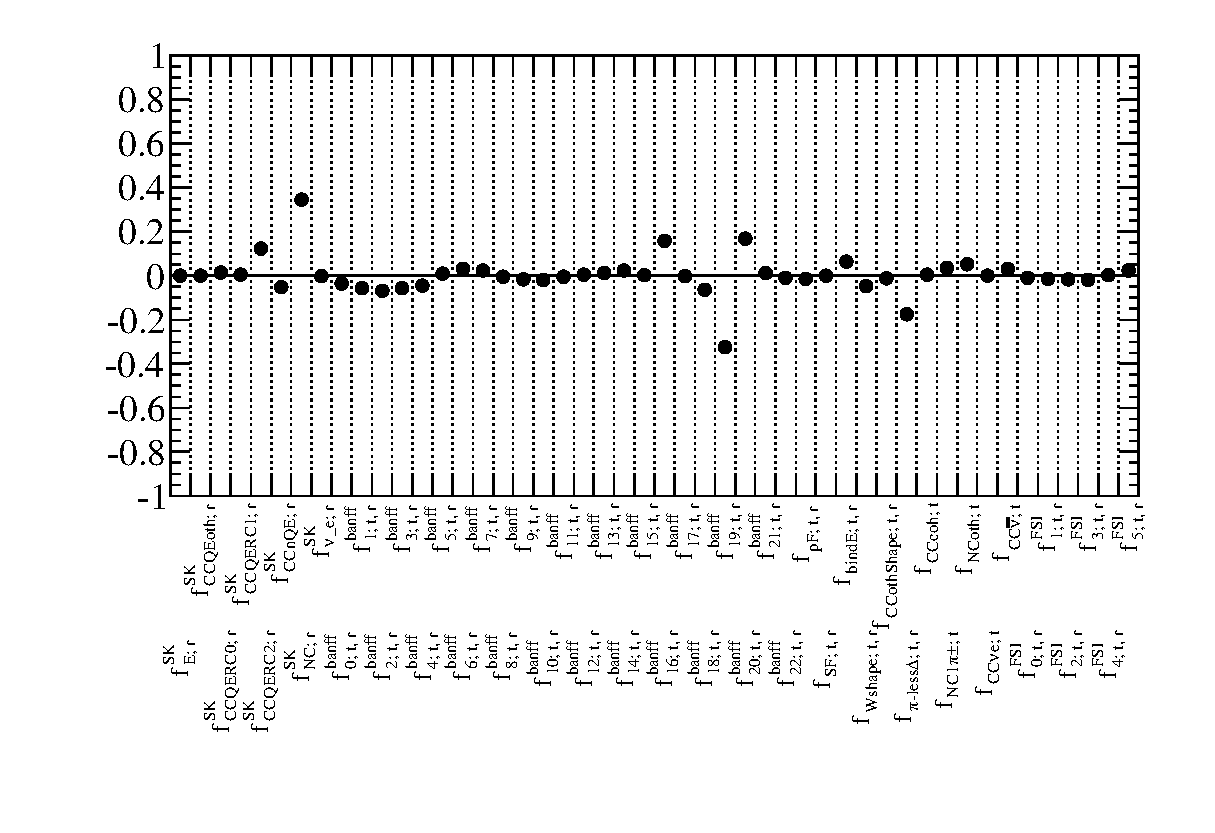
\includegraphics[width=50pc,angle=270]{./images/fit_data/2Nsintheta/pulls_3}
\caption {
  Systematic parameter pulls for the `2+N' $\sin^2\theta_{23}$ fit to the Run 1+2+3 dataset.
}
\label{fig:results_data123_pulls_2Nsintheta}
\end{figure*}

\begin{figure*}[htb]
\center
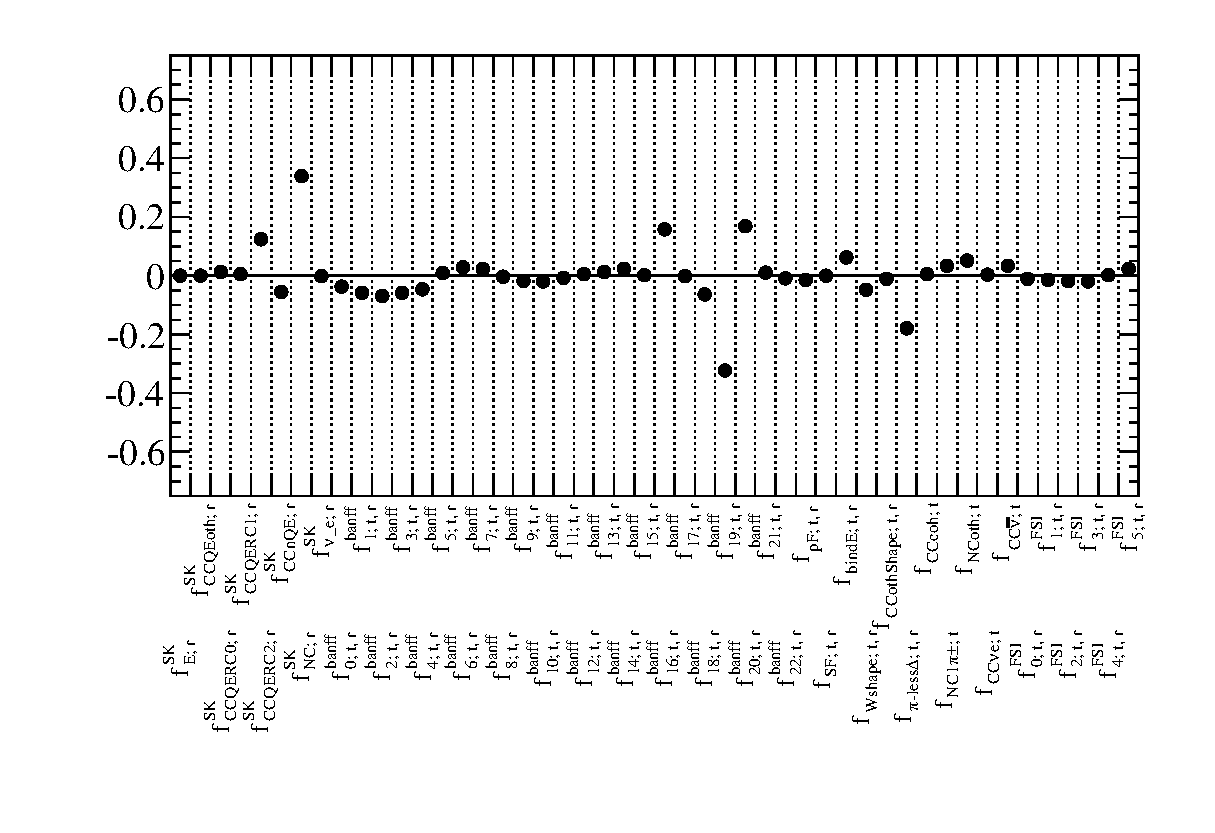
\includegraphics[width=50pc,angle=270]{./images/fit_data/2N/pulls_3}
\caption {
  Systematic parameter pulls for the `2+N' fit to the Run 1+2+3 dataset, assuming $\theta_{23}$ is in the first octant.
}
\label{fig:results_data123_pulls_2N}
\end{figure*}

\begin{figure*}[htb]
\center
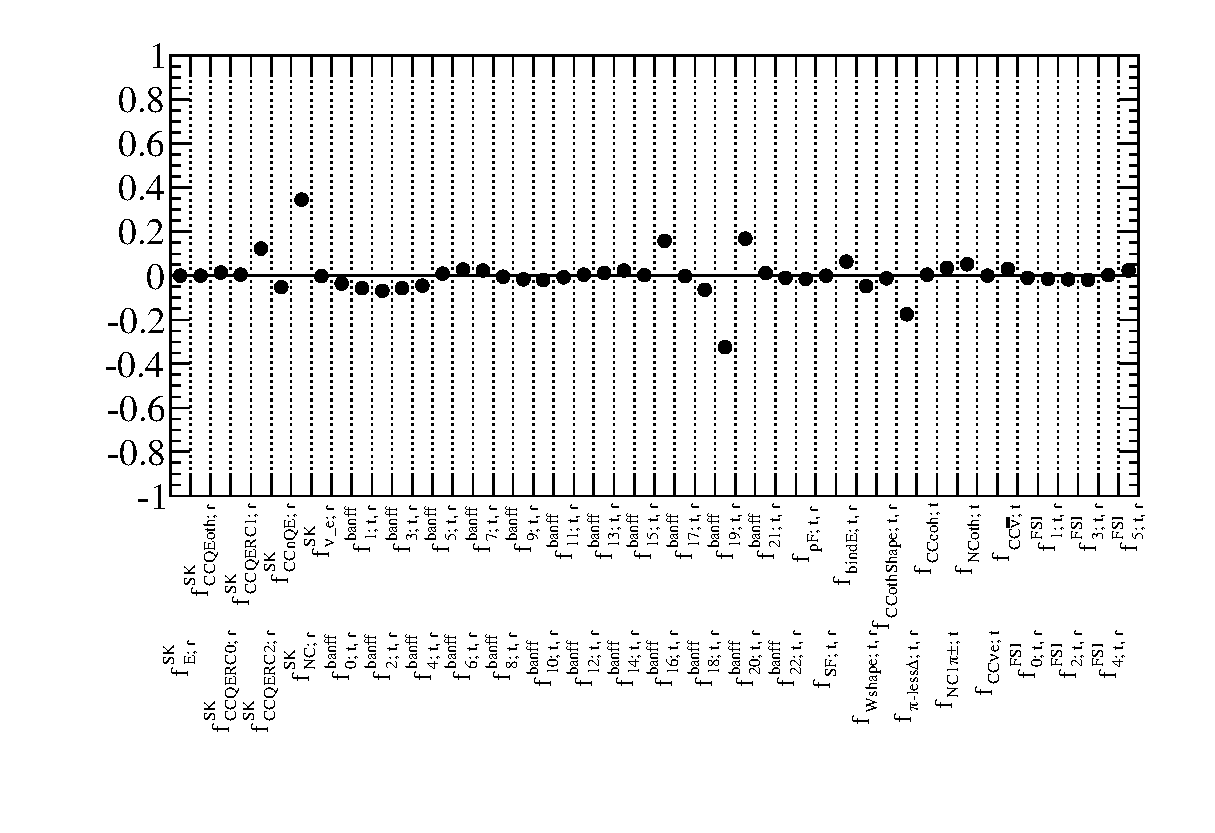
\includegraphics[width=50pc,angle=270]{./images/fit_data/2Noctant2/pulls_3}
\caption {
  Systematic parameter pulls for the `2+N' fit to the Run 1+2+3 dataset, assuming $\theta_{23}$ is in the second octant.
}
\label{fig:results_data123_pulls_2NO2}
\end{figure*}

\begin{figure*}[htb]
\begin{minipage}[t]{0.48\linewidth}
\center
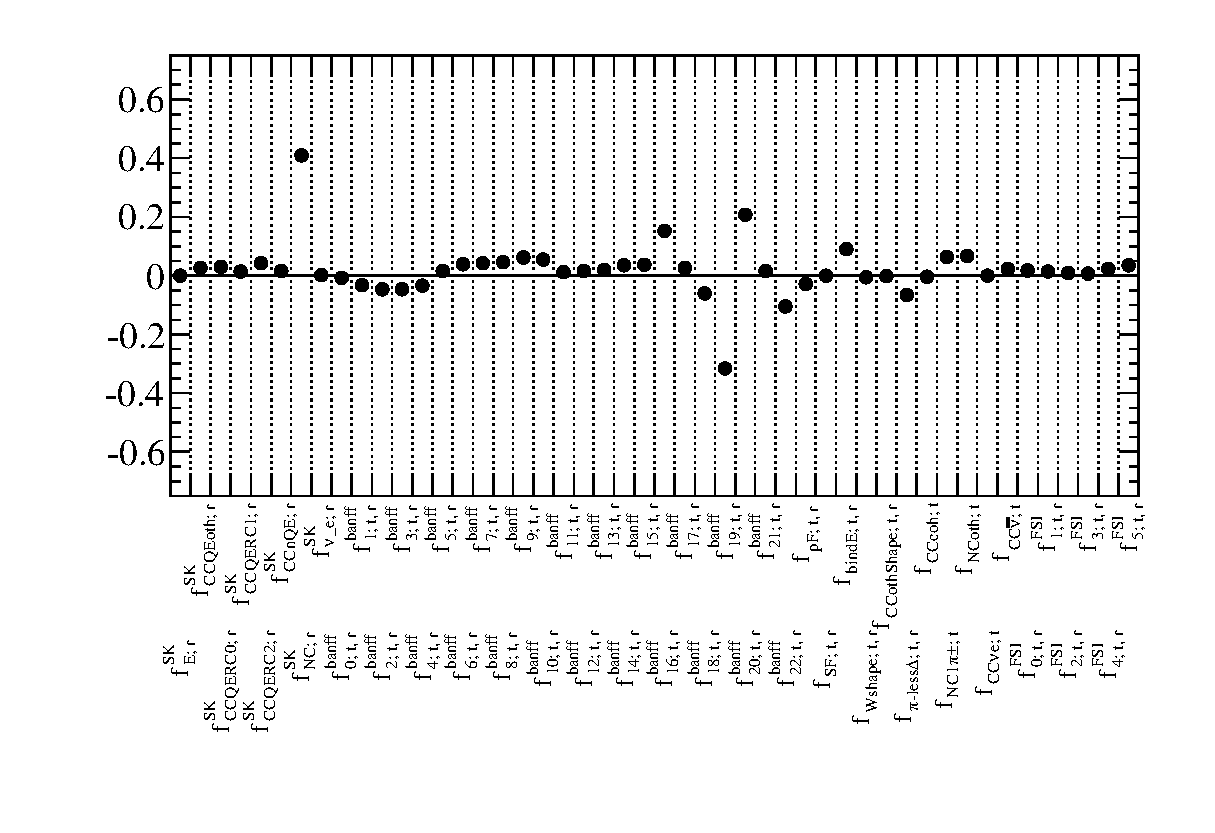
\includegraphics[width=22pc,angle=270]{./images/fit_data/2N/pulls_4}
\caption {
  Systematic parameter pulls for the `2+N' fit to the Run 1+2 dataset.
}
\label{fig:results_data12_pulls_2N}
\end{minipage}
\hspace{0.06\linewidth}
\begin{minipage}[t]{0.48\linewidth}
\center
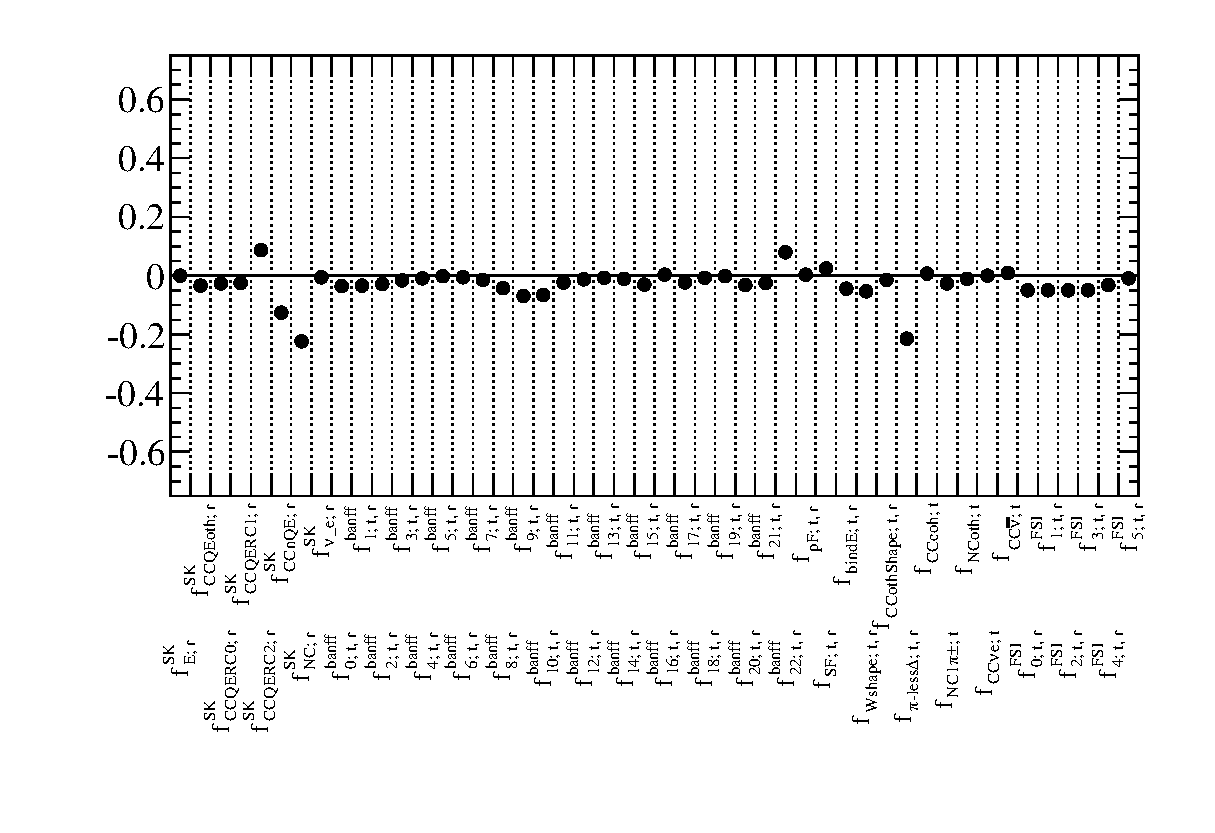
\includegraphics[width=22pc,angle=270]{./images/fit_data/2N/pulls_5}
\caption {
  Systematic parameter pulls for the `2+N' fit to the Run 3 dataset.
}
\label{fig:results_data3_pulls_2N}
\end{minipage}
\end{figure*}

%...........................................................
%
% Systematic parameter pulls for `2+8' fits
%
\clearpage
\begin{figure*}[htb]
\center
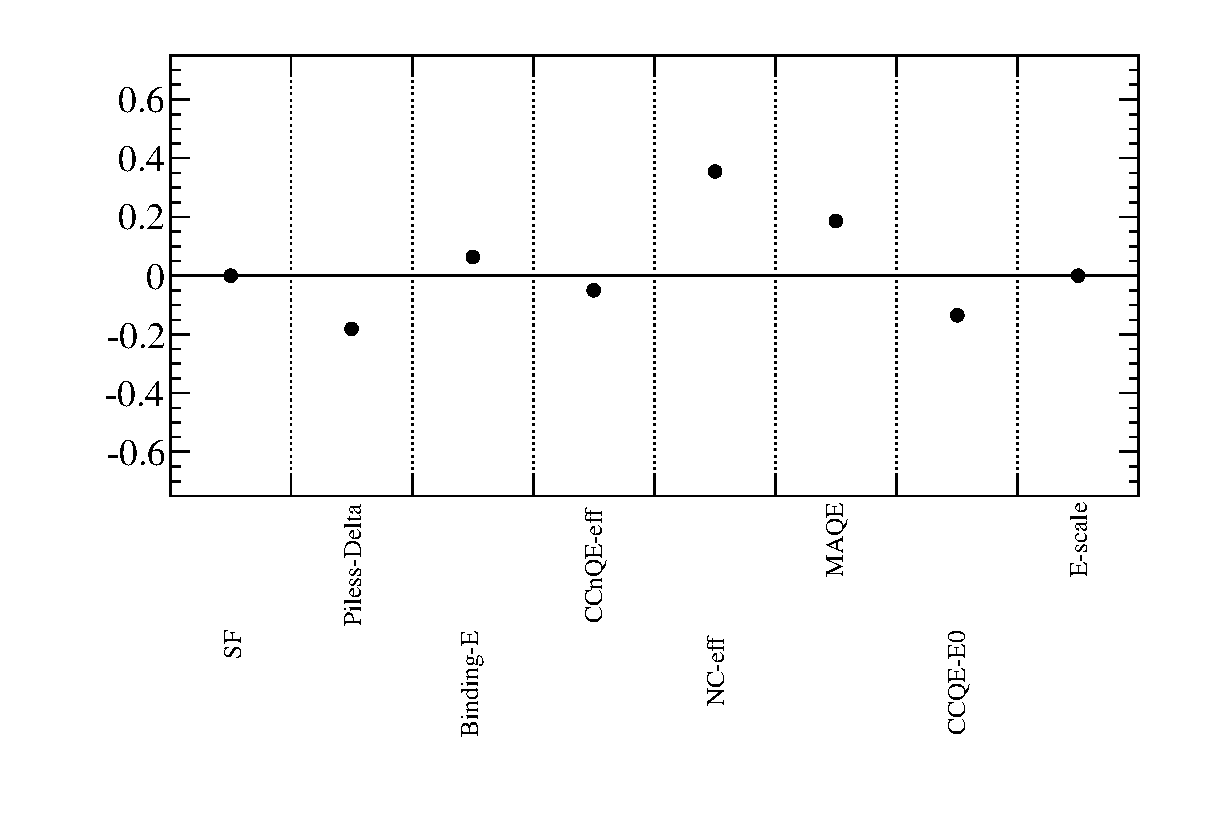
\includegraphics[width=25pc,angle=270]{./images/fit_data/28/pulls_3}
\caption {
  Systematic parameter pulls for the `2+8' fit to the Run 1+2+3 dataset.
}
\label{fig:results_data123_pulls}
\end{figure*}

\begin{figure*}[htb]
\begin{minipage}[t]{0.48\linewidth}
\center
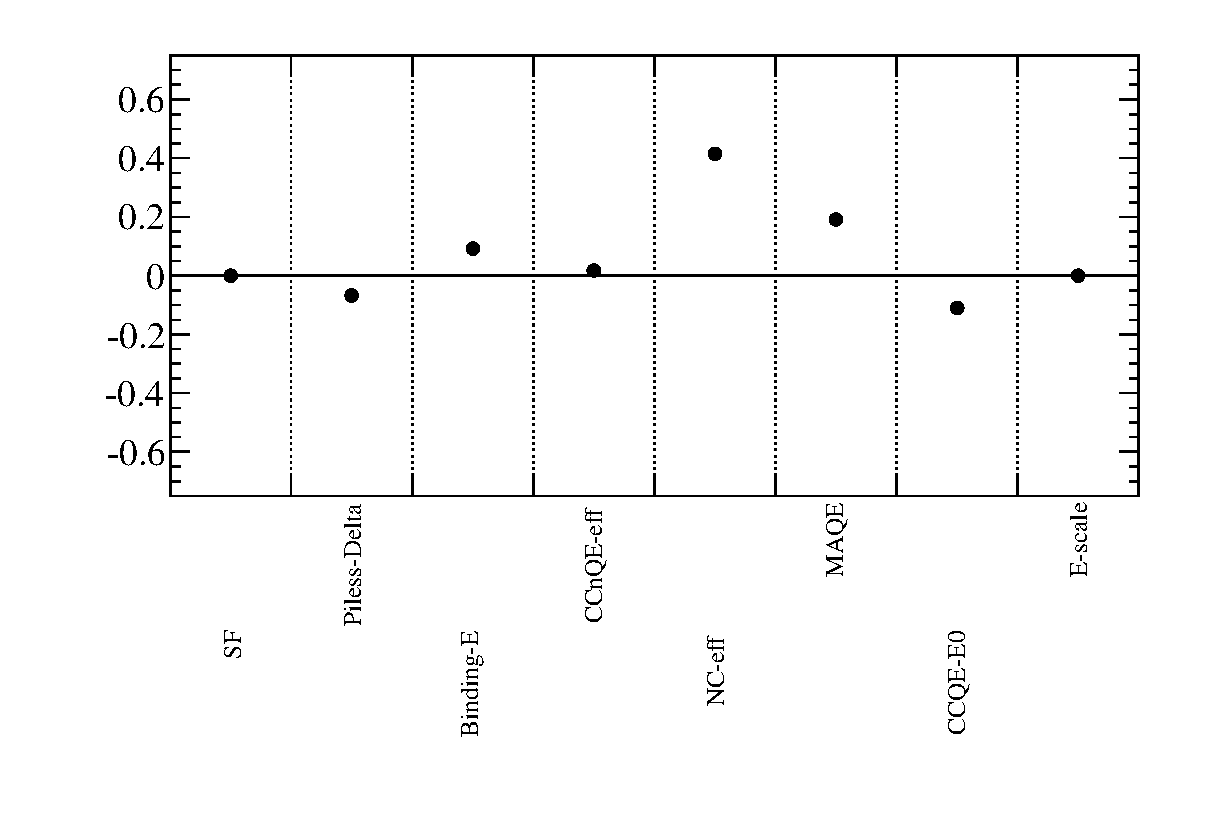
\includegraphics[width=20pc,angle=270]{./images/fit_data/28/pulls_4}
\caption {
  Systematic parameter pulls for the `2+8' fit to the Run 1+2 dataset.
}
\label{fig:results_data12_pulls}
\end{minipage}
\hspace{0.06\linewidth}
\begin{minipage}[t]{0.48\linewidth}
\center
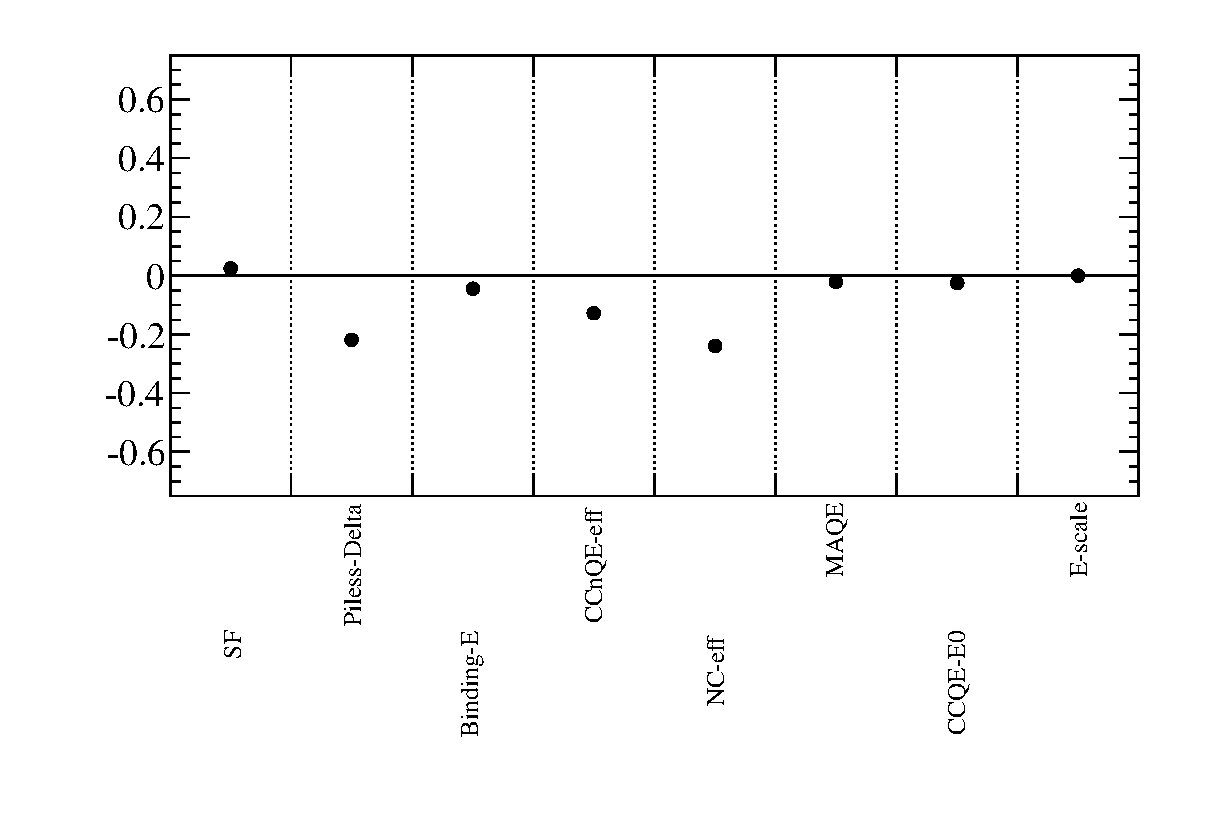
\includegraphics[width=20pc,angle=270]{./images/fit_data/28/pulls_5}
\caption {
  Systematic parameter pulls for the `2+8' fit to the Run 3 dataset.
}
\label{fig:results_data3_pulls}
\end{minipage}
\end{figure*}

%--------------------------------------------------------------------------------------
% Goodness of fit tests
%--------------------------------------------------------------------------------------

\clearpage
\subsection {Goodness-of-fit tests}
\label{sec:results_gof}

Goodness-of-fit tests were performed as described in Sec.\ \ref{sec:gof_test},
and the p-values for all `2+N' and `2+8' $\sin^22\theta_{23}$ fits to the Run 1+2+3, Run 1+2 and Run 3
datasets are shown in Tab.\ \ref{tab:data_fits:best_fit_values}. The $\chi^2$ distributions from 
which the p-values were calculated are shown for the `2+N' fit
for $\sin^2\theta_{23}$ in Fig.\ \ref{fig:results_data123_goodness_2Nsintheta},
for the '2+N' fit assuming the first and second octants for $\theta_{23}$ for
Run 1+2+3 data in Figs.\ \ref{fig:results_data123_goodness_2N} and \ref{fig:results_data123_goodness_2NO2} respectively,
and for the '2+8' fit for Run 1+2+3 data in Fig.\ \ref{fig:results_data123_goodness}.
All fits have a high degree of plausibility.

%..................................
%
% Summary table with fit p-values
%
%\begin{table}
%\centering
%\begin{tabular}{| l | l | c |}
%\hline
%Analysis                 & Run period & p-value \\
%\hline
%2012 / 3-flavour / `2+N' & Run 1+2+3   & 0.83 \\
%2012 / 3-flavour / `2+8' & Run 1+2+3   & 0.82 \\
%\hline
%2012 / 3-flavour / `2+N' & Run 3       & 0.83 \\
%2012 / 3-flavour / `2+8' & Run 3       & 0.63 \\
%\hline
%2012 / 3-flavour / `2+N' & Run 1+2     & 0.82 \\
%2012 / 3-flavour / `2+8' & Run 1+2     & 0.68 \\
%\hline
%\end{tabular}
%\caption{
%  Summary of p-values obtained from the goodness-of-fit test of Sec.\ \ref{sec:gof_test}
%  for both `2+N' and `2+8' oscillation fits to the Run 1+2, Run 3, and combined Run 1+2+3 datasets.
%}
%\label{tab:data_fit:gof}
%\end{table}
%


%..................................
%
% Chisq_{gof} distributions
%

\begin{figure*}[htb]
\begin{minipage}[t]{0.48\linewidth}
\center
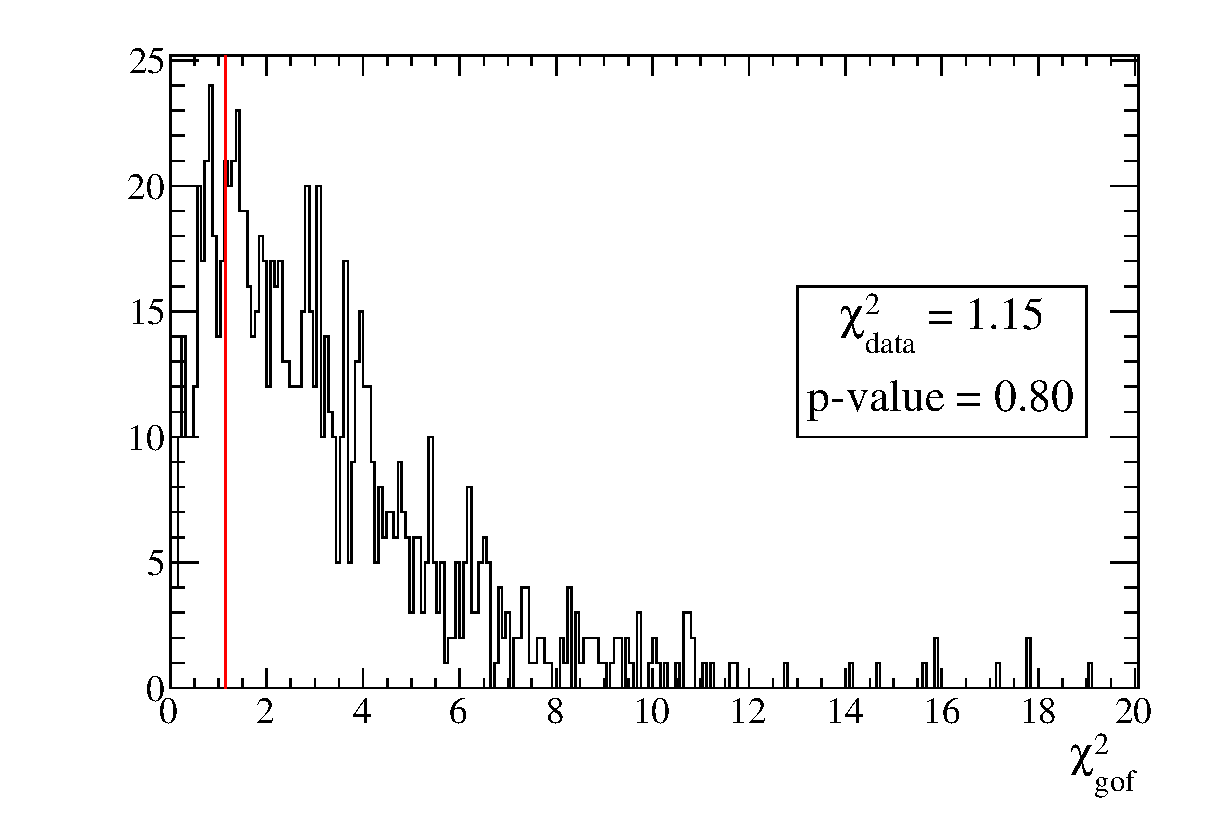
\includegraphics[width=18pc]{./images/fit_data/2Nsintheta/goodness_3}
\caption {
  Distribution of $\chi^2_{gof}$, the goodness-of-fit (gof) $\chi^2$, 
  from 1k toy MC experiments generated at the `2+N' $\sin^2\theta_{23}$ Run 1+2+3 best-fit oscillation point.
  The $\chi^2_{gof}$ value for the Run 1+2+3 data ($\chi^2_{data}$) is highlighted.
}
\label{fig:results_data123_goodness_2Nsintheta}
\end{minipage}
\hspace{0.06\linewidth}
\begin{minipage}[t]{0.48\linewidth}
\center
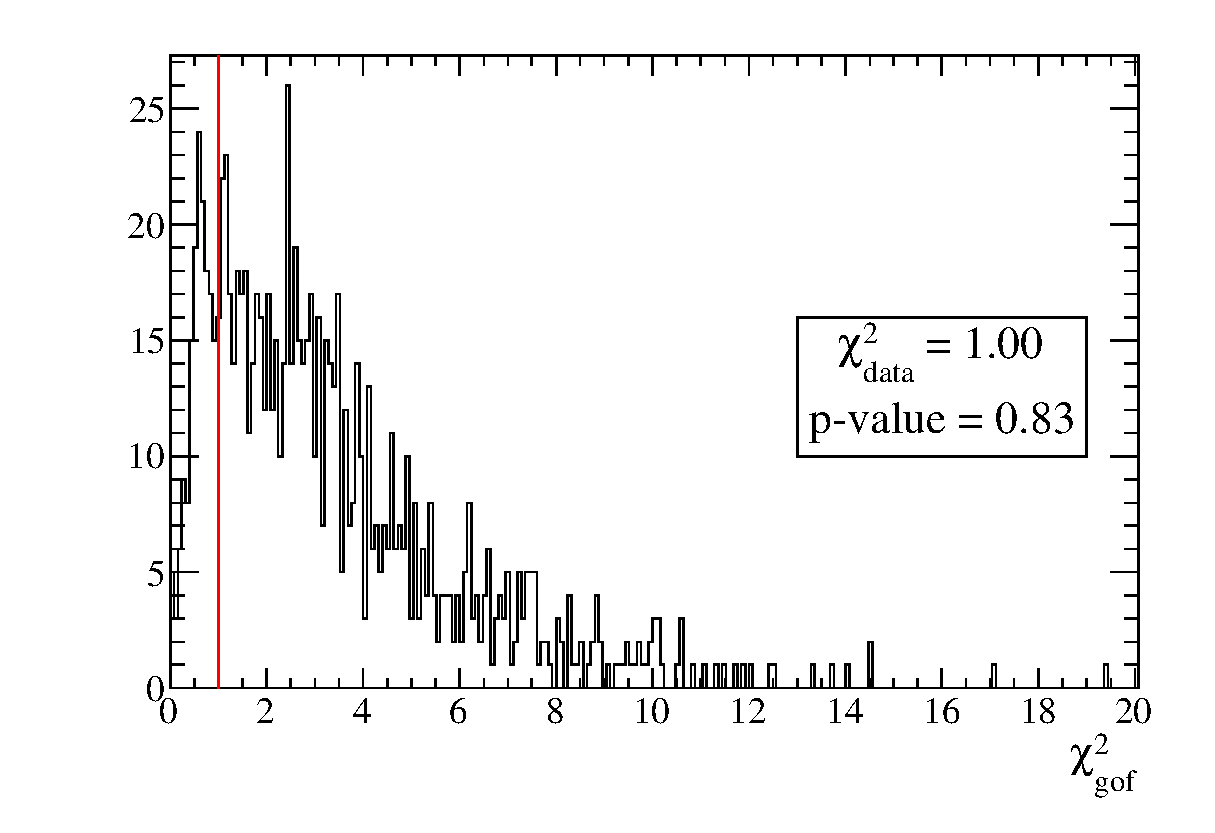
\includegraphics[width=18pc]{./images/fit_data/2N/goodness_3}
\caption {
  As in Fig.\ \ref{fig:results_data123_goodness_2Nsintheta}, but for the `2+N' fit to the Run 1+2+3 dataset
  assuming $\theta_{23}$ is in the first octant.
}
\label{fig:results_data123_goodness_2N}
\end{minipage}
\end{figure*}


\begin{figure*}[htb]
\begin{minipage}[t]{0.48\linewidth}
\center
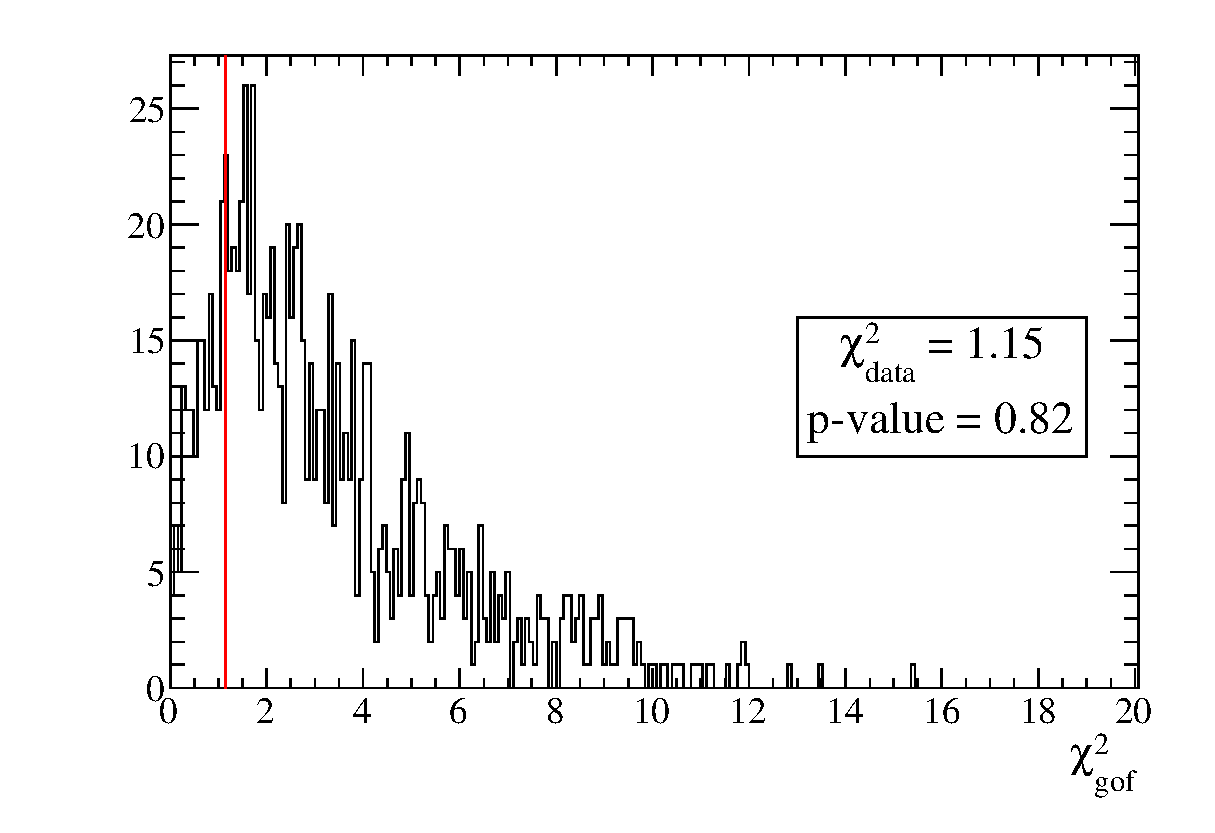
\includegraphics[width=18pc]{./images/fit_data/2Noctant2/goodness_3}
\caption {
  As in Fig.\ \ref{fig:results_data123_goodness_2Nsintheta}, but for the `2+N' fit to the Run 1+2+3 dataset
  assuming $\theta_{23}$ is in the second octant.
}
\label{fig:results_data123_goodness_2NO2}
\end{minipage}
\hspace{0.06\linewidth}
\begin{minipage}[t]{0.48\linewidth}
\center
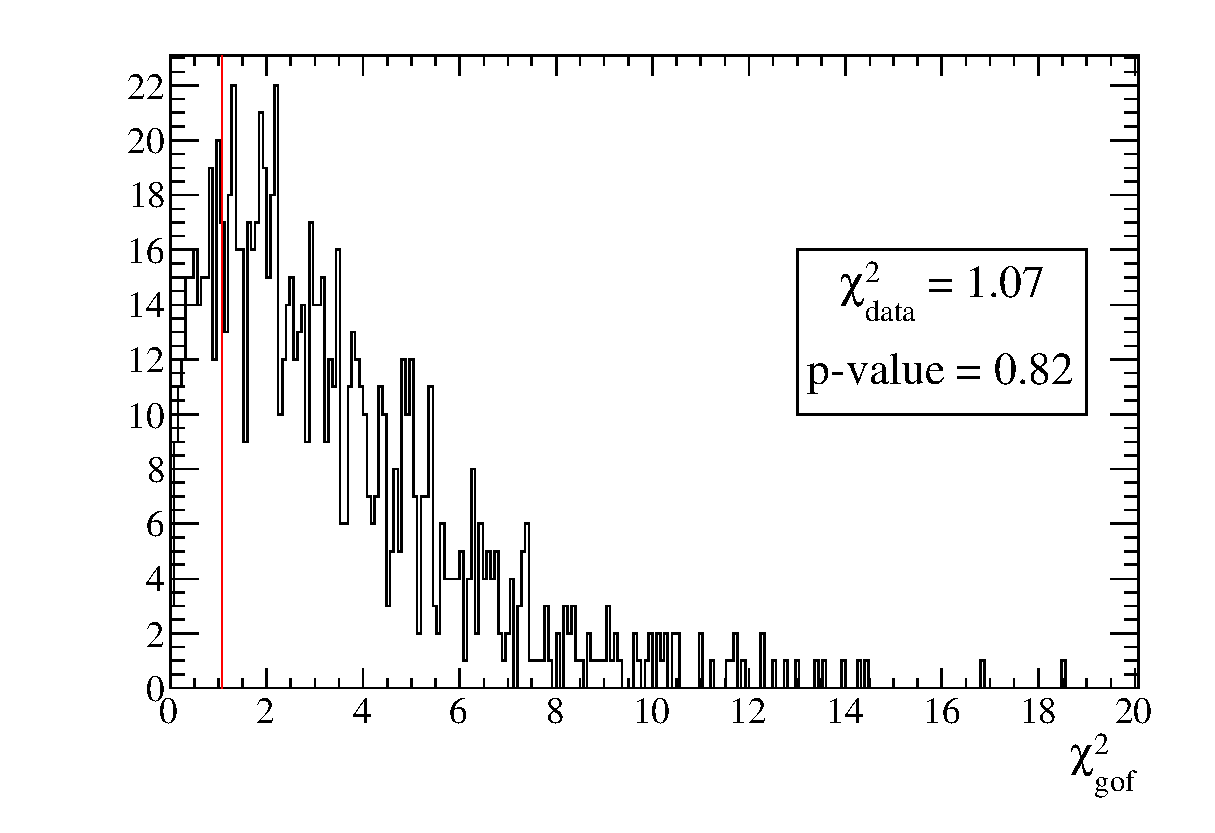
\includegraphics[width=18pc]{./images/fit_data/28/goodness_3}
\caption {
  As in Fig.\ \ref{fig:results_data123_goodness_2Nsintheta}, but for the `2+8' fit to the Run 1+2+3 dataset.
}
\label{fig:results_data123_goodness}
\end{minipage}
\end{figure*}


%--------------------------------------------------------------------------------------
% Best-fit spectra
%--------------------------------------------------------------------------------------

\subsection {Best-fit single $\mu$-like ring reconstructed energy spectra}
\label{sec:results_bestfit_spectra}

The reconstructed neutrino energy distribution of the single $\mu$-like ring events in the Run 1+2+3 dataset is shown in Fig.\ 
\ref{fig:results_data123_spectrum_2Nsintheta} along with the `2+N' $\sin^2\theta_{23}$ best-fit prediction and
the prediction made under the no-oscillation 
hypothesis. Also shown is the ratio between the data and the no-oscillation spectrum and the ratio between the `2+N' $\sin^2\theta_{23}$ best-fit 
spectrum and the the no-oscillation spectrum; in both of these ratios, the characteristic energy-dependent deficit can be 
clearly seen.
The equivalent spectra for the Run 1+2+3 (assuming $\theta_{23}$ is in the first octant),
Run 1+2+3 (assuming $\theta_{23}$ is in the second octant),
Run 1+2 and Run 3 datasets are also shown in Figs.\ \ref{fig:results_data123_spectrum_2N}, \ref{fig:results_data123_spectrum_2NO2}, \ref{fig:results_data12_spectrum_2N} 
and \ref{fig:results_data3_spectrum_2N} respectively. All these distribution are shown in the 73-bin scheme in reconstructed 
neutrino energy that was used in the fitting procedure (see Sec.\ \ref{sec:mc_templates:template_binning}).

`2+8' fits were also made to the Run 1+2+3, Run 1+2 and Run 3 datasets. The best-fit and no-oscillation spectra are compared with 
the data in in Figs.\
\ref{fig:results_data123_spectrum},  
\ref{fig:results_data12_spectrum} and
\ref{fig:results_data3_spectrum}.
The ratios of the data and best-fit spectra to the no-oscillation spectra are also shown in these figures, and the energy-dependent 
deficits are once more clearly visible. 

Since the reconstructed energy binning used in the fit is relatively fine, it can be beneficial to see the above distributions using 
a coarser binning. The best-fit spectra obtained for the Run 1+2+3 dataset from the `2+N' fit for $\sin^2\theta_{23}$,
the '2+N' fit with $\theta_{23}$ in the first octant, 
the '2+N' fit with $\theta_{23}$ in the second octant and the `2+8' fit with $\theta_{23}$ in the first octant are shown using a coarse 
binning\footnote{
  16 reconstructed energy bins arranged as follows:
  1 0.3-GeV bin in 0 - 0.3 GeV,
  8 0.1-GeV bins in 0.3 - 1.1 GeV,
  1 0.15-GeV bin in 1.1 GeV - 1.25 GeV,
  1 0.25-GeV bin in 1.25 - 1.5 GeV GeV,
  1 0.5-GeV bin in 1.5 - 2 GeV,
  2 1-GeV bin in 2-4 GeV,
  1 2-GeV bin in 4-6 GeV and 1 bin above 6 GeV.
} 
in Figs.\
\ref{fig:results_data123_spectrum_coarse_2Nsintheta},
\ref{fig:results_data123_spectrum_coarse_2N},
\ref{fig:results_data123_spectrum_coarse_2NO2} and
\ref{fig:results_data123_spectrum_coarse}
respectively. It is also interesting to see the 28 components of the best-fit spectrum, each of which is calculated separately 
in this analysis. These components are shown for the `2+N' and `2+8' 
fits in Figs.\ 
\ref{fig:results_data123_spectrum_components_2Nsintheta},
\ref{fig:results_data123_spectrum_components_2N},
\ref{fig:results_data123_spectrum_components_2NO2} and
\ref{fig:results_data123_spectrum_components} respectively.
In these plots, the components of the spectrum are grouped into 5 categories: 
$\nu_{\mu}$ CCQE, $\nu_{\mu}$ CCnonQE, $\bar{\nu}_{\mu}$ CC, $\nu_{e}$/$\bar{\nu}_{e}$ CC and NC.

The '2+N' best-fit predictions for $\sin^2\theta_{23}$ and $\theta_{23}$ assuming the second octant
are compared for the Run 1+2+3 dataset only in  
Fig.\ \ref{fig:results_data123_spectrum_comparison_sintheta}, 
using the 73 reconstructed energy bins used in the fit, and in
Fig.\ \ref{fig:results_data123_spectrum_comparison_sintheta_coarse},
using the coarser binning described above.
The two best-fit spectra are nearly identical. In the 73-bin scheme used for the fit,
the spectra never differ by more than 0.1\% in the area below 3 GeV,
and they are nearly identical in the area of the first oscillation maximum.

The '2+N' best-fit predictions for both $\theta_{23}$ octant assumptions are compared for the Run 1+2+3 dataset only in  
Fig.\ \ref{fig:results_data123_spectrum_comparison_octant}, 
using the 73 reconstructed energy bins used in the fit, and in
Fig.\ \ref{fig:results_data123_spectrum_comparison_octant_coarse},
using the coarser binning described above.

Finally, the `2+N' and `2+8' best-fit predictions are compared for the Run 1+2+3 dataset only in  
Fig.\ \ref{fig:results_data123_spectrum_comparison}, 
using the 73 reconstructed energy bins used in the fit, and in
Fig.\ \ref{fig:results_data123_spectrum_comparison_coarse},
using the coarser binning described above.
The two best-fit spectra are nearly identical. In the 73-bin scheme used for the fit,
the spectra never differ by more than 1.5\% in the area below 3 GeV,
and they are nearly identical in the area of the first oscillation maximum.

%...........................................................
%
% Best-fit spectra and ratios for `2+N' fits (73 bins)
%
\begin{figure*}[htb]
\center
\includegraphics[width=28pc]{./images/fit_data/2Nsintheta/spectrum_3}
\caption {
  Best-fit reconstructed energy spectrum (top) obtained from the `2+N' $\sin^2\theta_{23}$ fit to the combined Run 1+2+3 dataset.
  The Run 1+2+3 dataset and the prediction obtained from the no-oscillation hypothesis are also shown.
  The spectra are shown using the 73 bins used in the fit (see Sec.\ \ref{sec:mc_templates:template_binning}).
  The ratio of the data and best-fit distribution to the no-oscillation hypothesis is shown 
  in the bottom plot. The characteristic energy-dependent deficit can be clearly seen.
}
\label{fig:results_data123_spectrum_2Nsintheta}
\end{figure*}

\begin{figure*}[htb]
\center
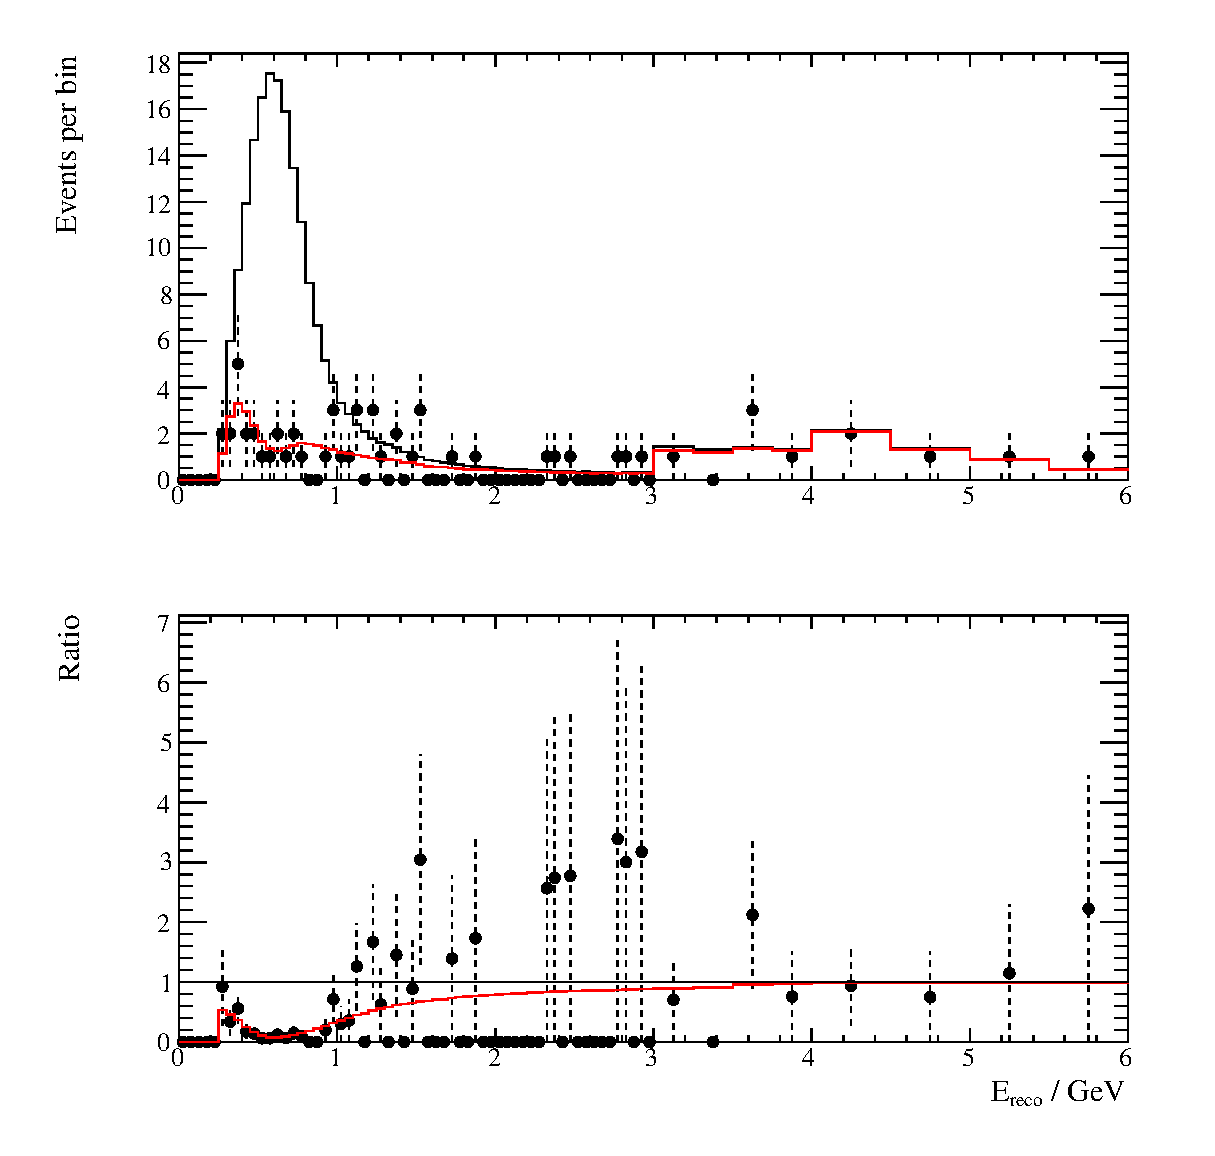
\includegraphics[width=28pc]{./images/fit_data/2N/spectrum_3}
\caption {
  Best-fit reconstructed energy spectrum (top) obtained from the `2+N' fit to the combined Run 1+2+3 dataset.
  The Run 1+2+3 dataset and the prediction obtained from the no-oscillation hypothesis are also shown.
  The spectra are shown using the 73 bins used in the fit (see Sec.\ \ref{sec:mc_templates:template_binning}).
  The ratio of the data and best-fit distribution to the no-oscillation hypothesis is shown 
  in the bottom plot. The characteristic energy-dependent deficit can be clearly seen.
}
\label{fig:results_data123_spectrum_2N}
\end{figure*}

\begin{figure*}[htb]
\center
\includegraphics[width=28pc]{./images/fit_data/2Noctant2/spectrum_3}
\caption {
  Best-fit reconstructed energy spectrum (top) obtained from the `2+N' fit to the combined Run 1+2+3 dataset,
  assuming $\theta_{23}$ is in the second octant.
  The Run 1+2+3 dataset and the prediction obtained from the no-oscillation hypothesis are also shown.
  The spectra are shown using the 73 bins used in the fit (see Sec.\ \ref{sec:mc_templates:template_binning}).
  The ratio of the data and best-fit distribution to the no-oscillation hypothesis is shown 
  in the bottom plot. The characteristic energy-dependent deficit can be clearly seen.
}
\label{fig:results_data123_spectrum_2NO2}
\end{figure*}

\begin{figure*}[htb]
\begin{minipage}[t]{0.48\linewidth}
\center
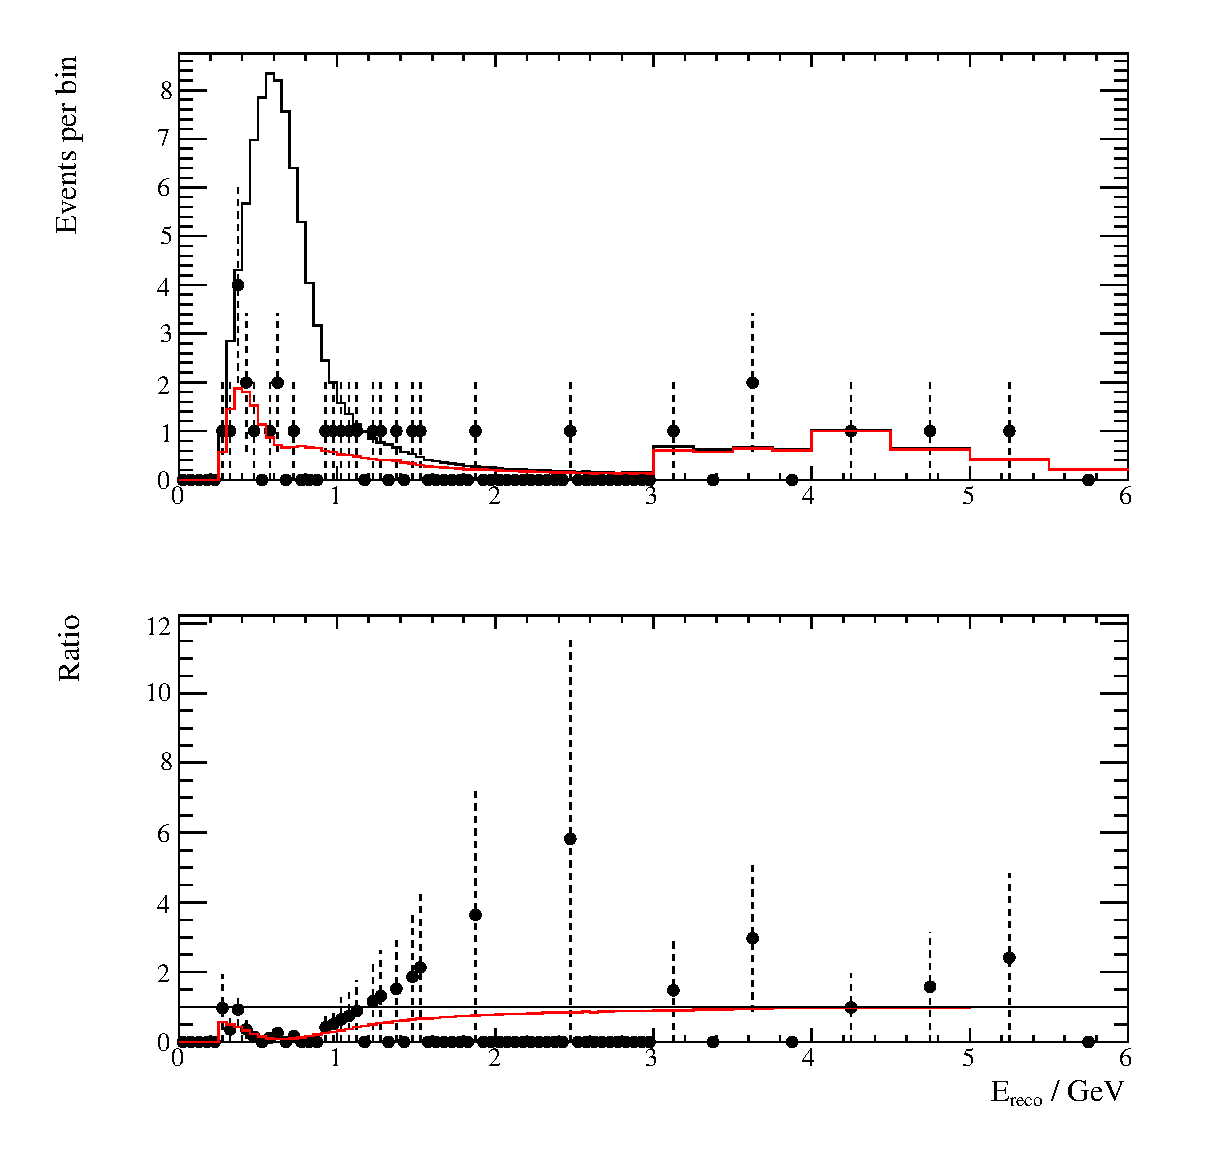
\includegraphics[width=20pc]{./images/fit_data/2N/spectrum_4}
\caption {
  As in Fig.\ \ref{fig:results_data123_spectrum_2N}, but for the Run 1+2 dataset only.
}
\label{fig:results_data12_spectrum_2N}
\end{minipage}
\hspace{0.06\linewidth}
\begin{minipage}[t]{0.48\linewidth}
\center
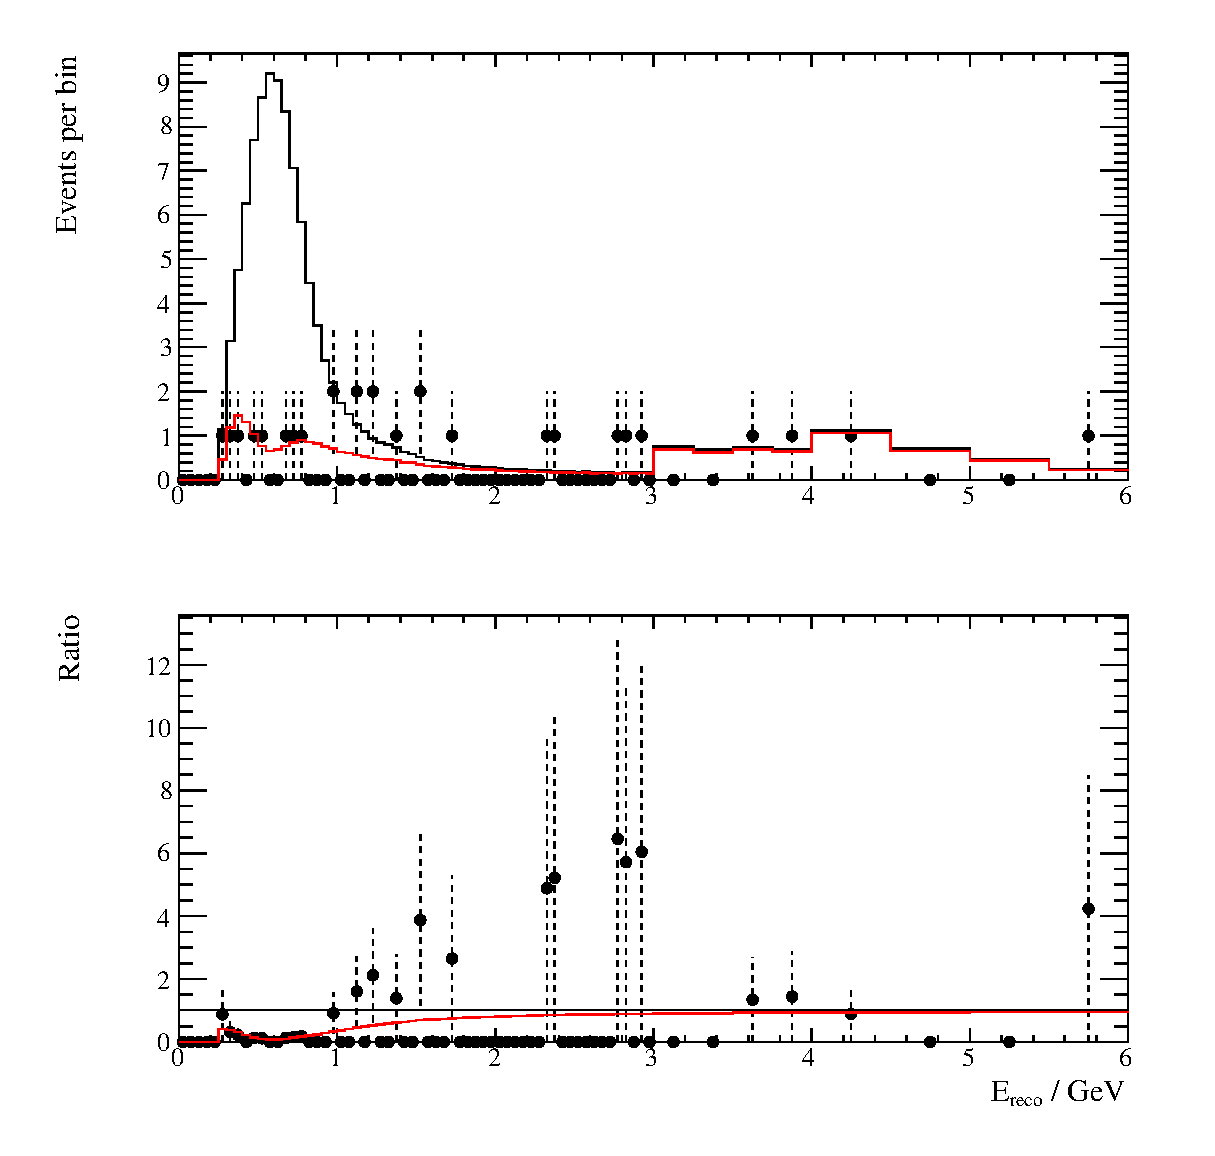
\includegraphics[width=20pc]{./images/fit_data/2N/spectrum_5}
\caption {
  As in Fig.\ \ref{fig:results_data123_spectrum_2N}, but for the Run 3 dataset only.
}
\label{fig:results_data3_spectrum_2N}
\end{minipage}
\end{figure*}


% ...........................................................
%
% Best-fit spectra and ratios for `2+8' fits (73 bins)
%
\begin{figure*}[htb]
\center
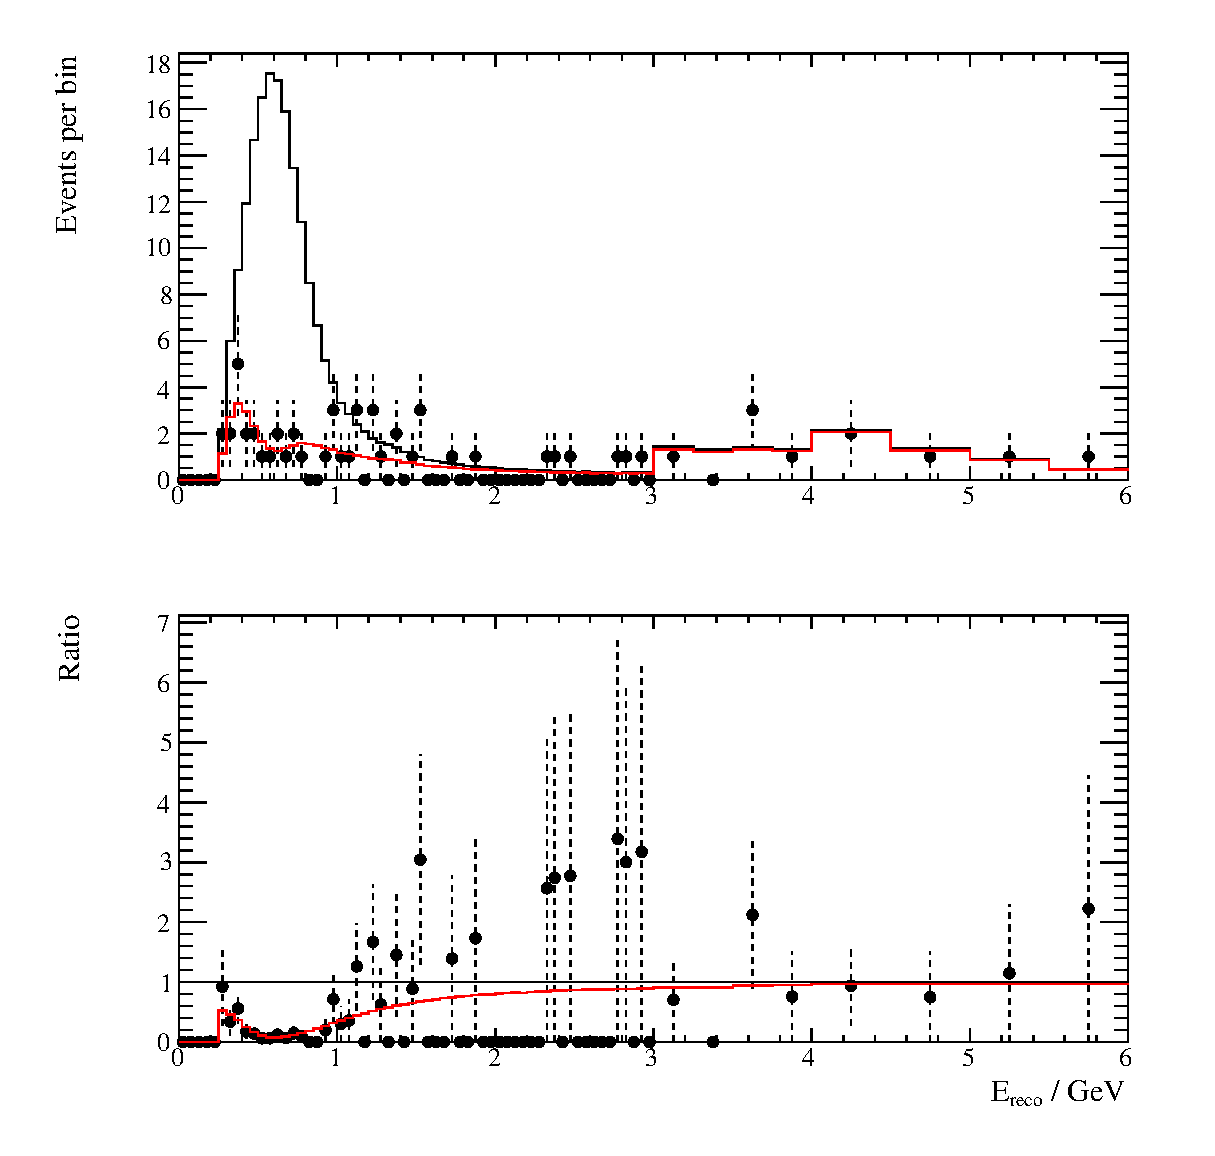
\includegraphics[width=28pc]{./images/fit_data/28/spectrum_3}
\caption {
  Best-fit reconstructed energy spectrum (top) obtained from the `2+8' fit to the combined Run 1+2+3 dataset.
  The Run 1+2+3 dataset and the prediction obtained from the no-oscillation hypothesis are also shown.
  The spectra are shown using the 73 bins used in the fit (see Sec.\ \ref{sec:mc_templates:template_binning}).
  The ratio of the data and best-fit distribution to the no-oscillation hypothesis is shown 
  in the bottom plot. The characteristic energy-dependent deficit can be clearly seen.
}
\label{fig:results_data123_spectrum}
\end{figure*}

\begin{figure*}[htb]
\begin{minipage}[t]{0.48\linewidth}
\center
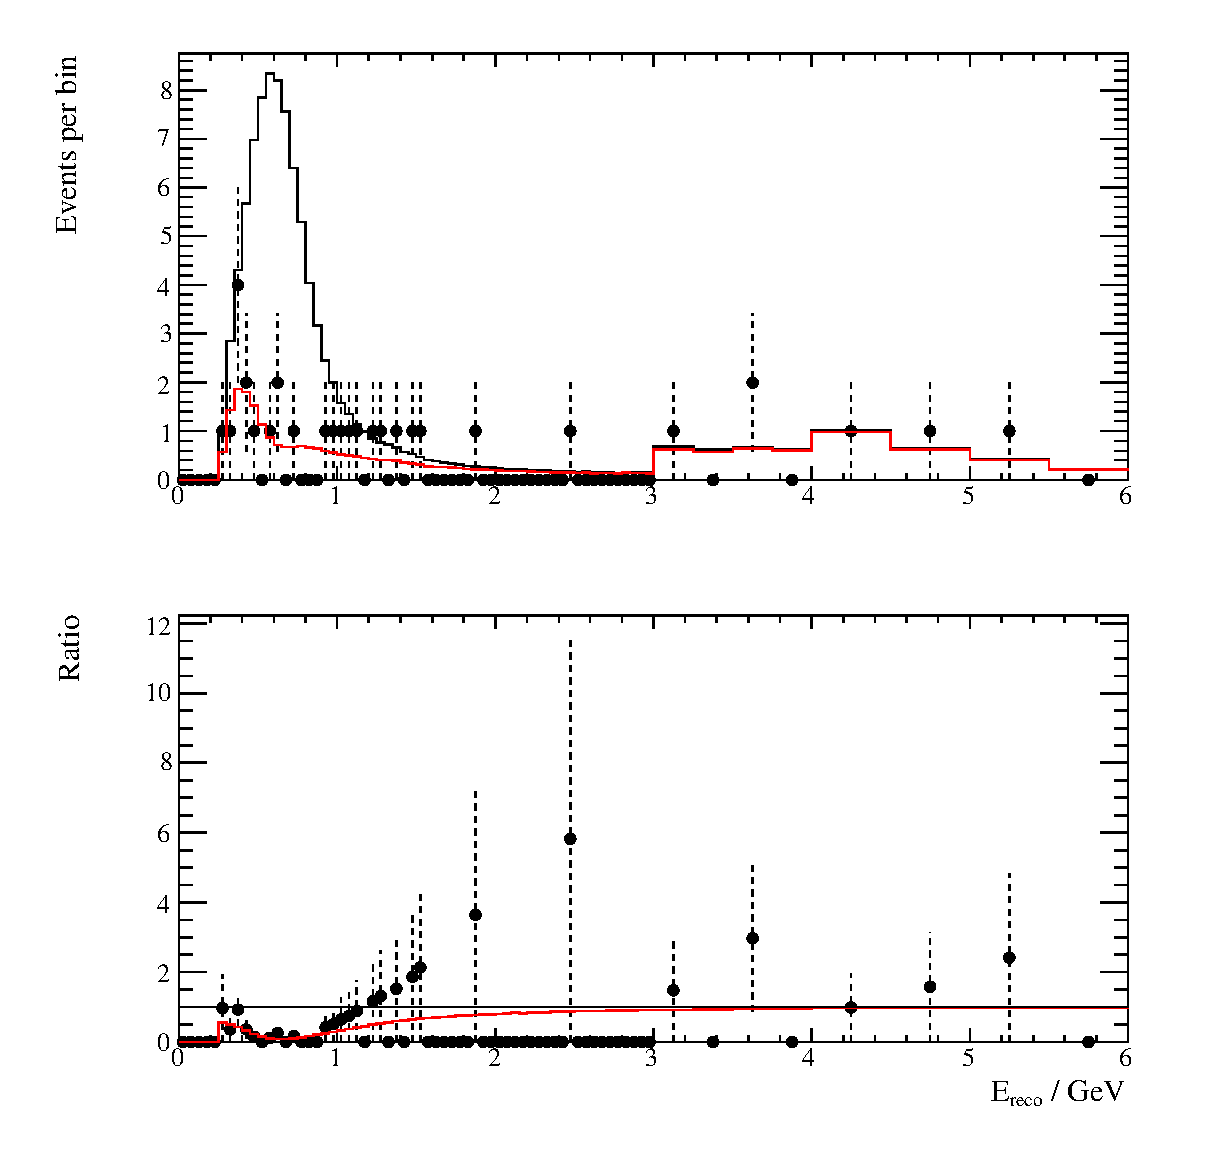
\includegraphics[width=20pc]{./images/fit_data/28/spectrum_4}
\caption {
  As in Fig.\ \ref{fig:results_data123_spectrum}, but for the Run 1+2 dataset only.
}
\label{fig:results_data12_spectrum}
\end{minipage}
\hspace{0.06\linewidth}
\begin{minipage}[t]{0.48\linewidth}
\center
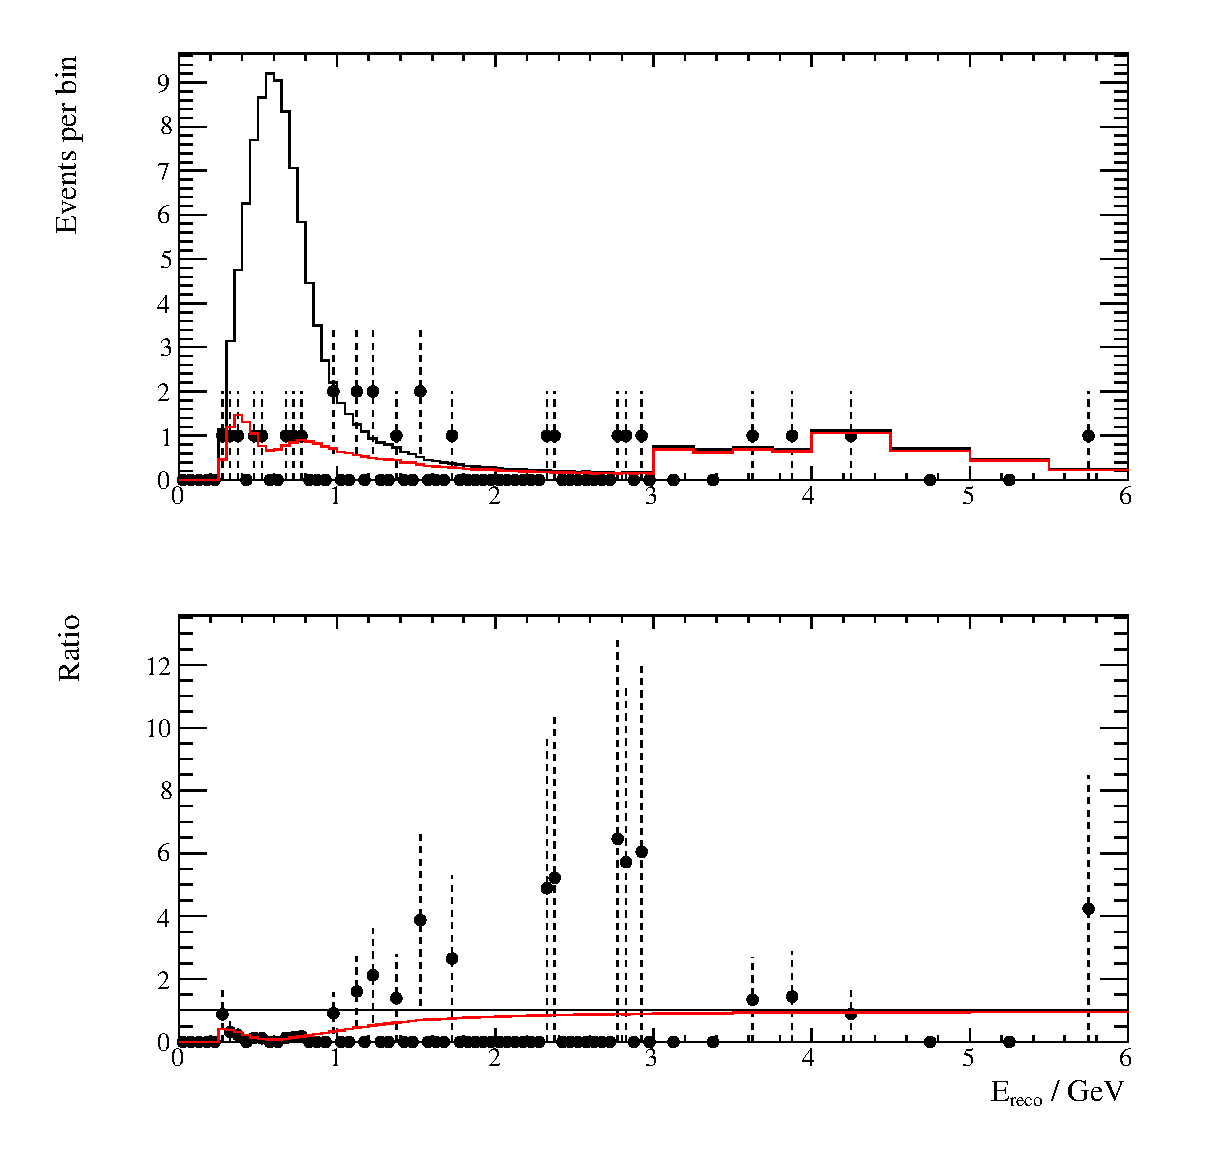
\includegraphics[width=20pc]{./images/fit_data/28/spectrum_5}
\caption {
  As in Fig.\ \ref{fig:results_data123_spectrum}, but for the Run 3 dataset only.
}
\label{fig:results_data3_spectrum}
\end{minipage}
\end{figure*}

%...........................................................
%
% Best-fit spectra (total and components) and ratios for `2+N' fit in sintheta
% (Run1+2+3 only, coarse binning)
%

\begin{figure*}[htb]
\center
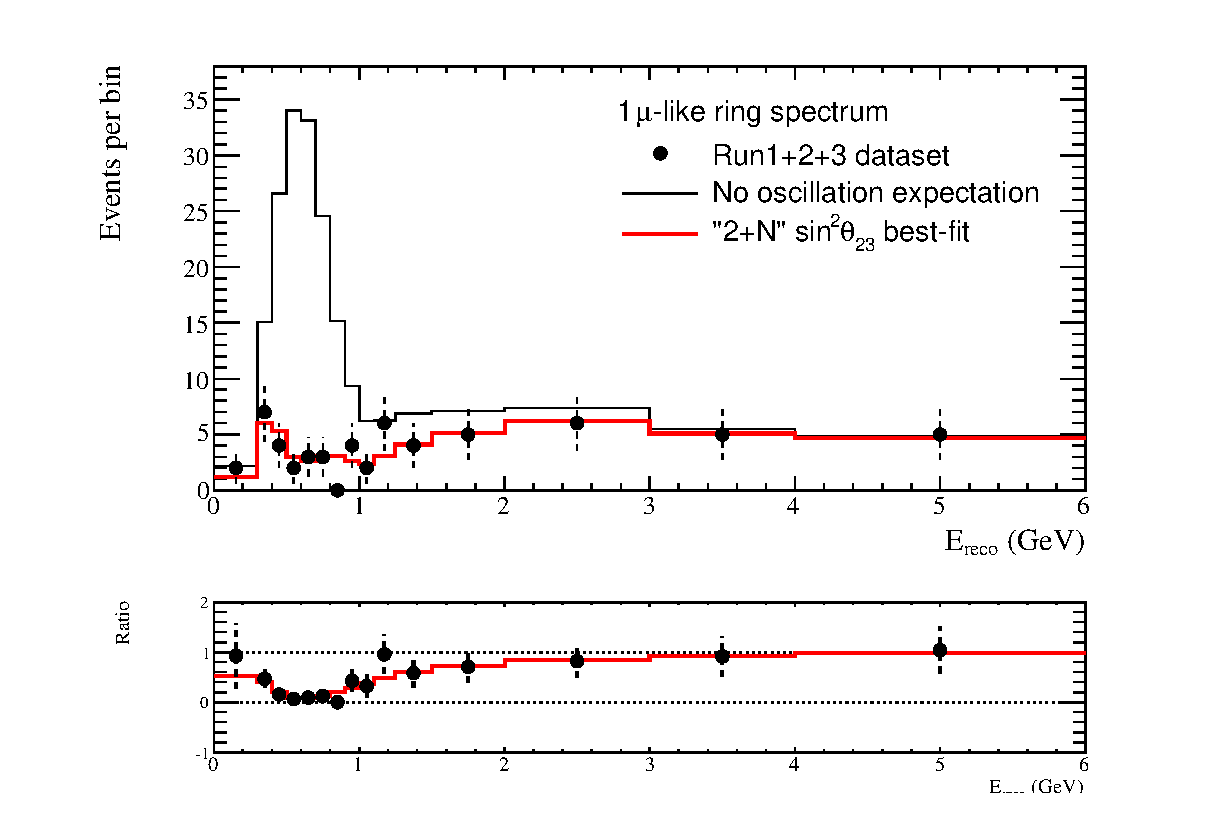
\includegraphics[width=34pc]{./images/fit_data/2Nsintheta/spectrum_and_ratio_2Nsintheta_coarse.eps}
\caption {
  Best-fit reconstructed energy spectrum using the coarse binning scheme (see 
  Sec.\ \ref{sec:results_bestfit_spectra}) obtained from the `2+N' $\sin^2\theta_{23}$ fit to the Run 1+2+3 dataset.
  Also shown are the spectrum obtained under the no-oscillation hypothesis
  and the ratios of the data and best-fit spectrum to it.
}
\label{fig:results_data123_spectrum_coarse_2Nsintheta}
\end{figure*}

\begin{figure*}[htb]
\center
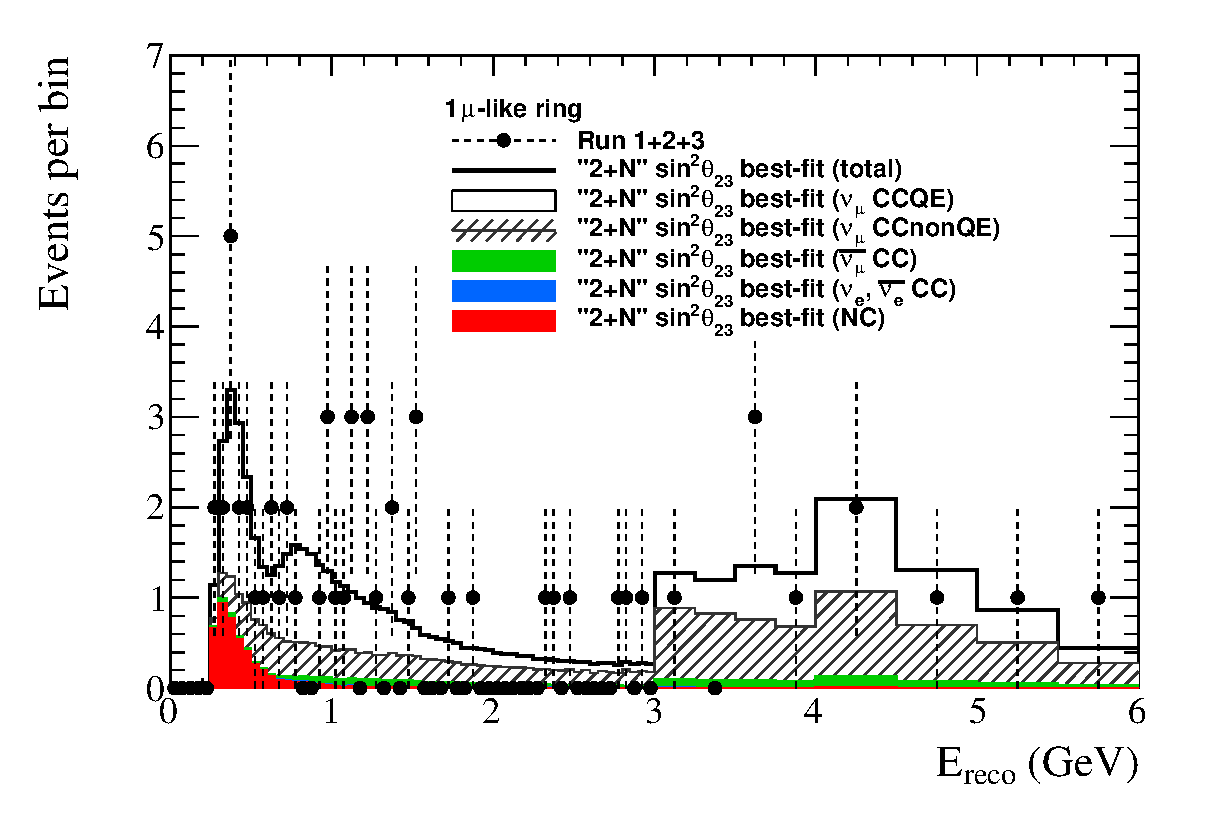
\includegraphics[width=24pc]{./images/fit_data/2Nsintheta/bestfit_spectrum_with_modes_run123_2Nsintheta.eps}
\caption {
  Best-fit reconstructed energy spectrum in the 73-bin scheme used in the fit (see 
  Sec.\ \ref{sec:mc_templates:template_binning}) and its components
  obtained from the `2+N' $\sin^2\theta_{23}$ fit to the Run 1+2+3 dataset.  
  The 28 components, each of which is calculated separately, are grouped into just 5 categories:
  $\nu_{\mu}$ CCQE, $\nu_{\mu}$ CCnQE, $\bar{\nu_{\mu}}$ CC, $\nu_{e}$/$\bar{\nu_{e}}$ CC and NC.  
}
\label{fig:results_data123_spectrum_components_2Nsintheta}
\end{figure*}


%...........................................................
%
% Best-fit spectra (total and components) and ratios for `2+N' fit 
% (Run1+2+3 only, coarse binning)
%

\begin{figure*}[htb]
\center
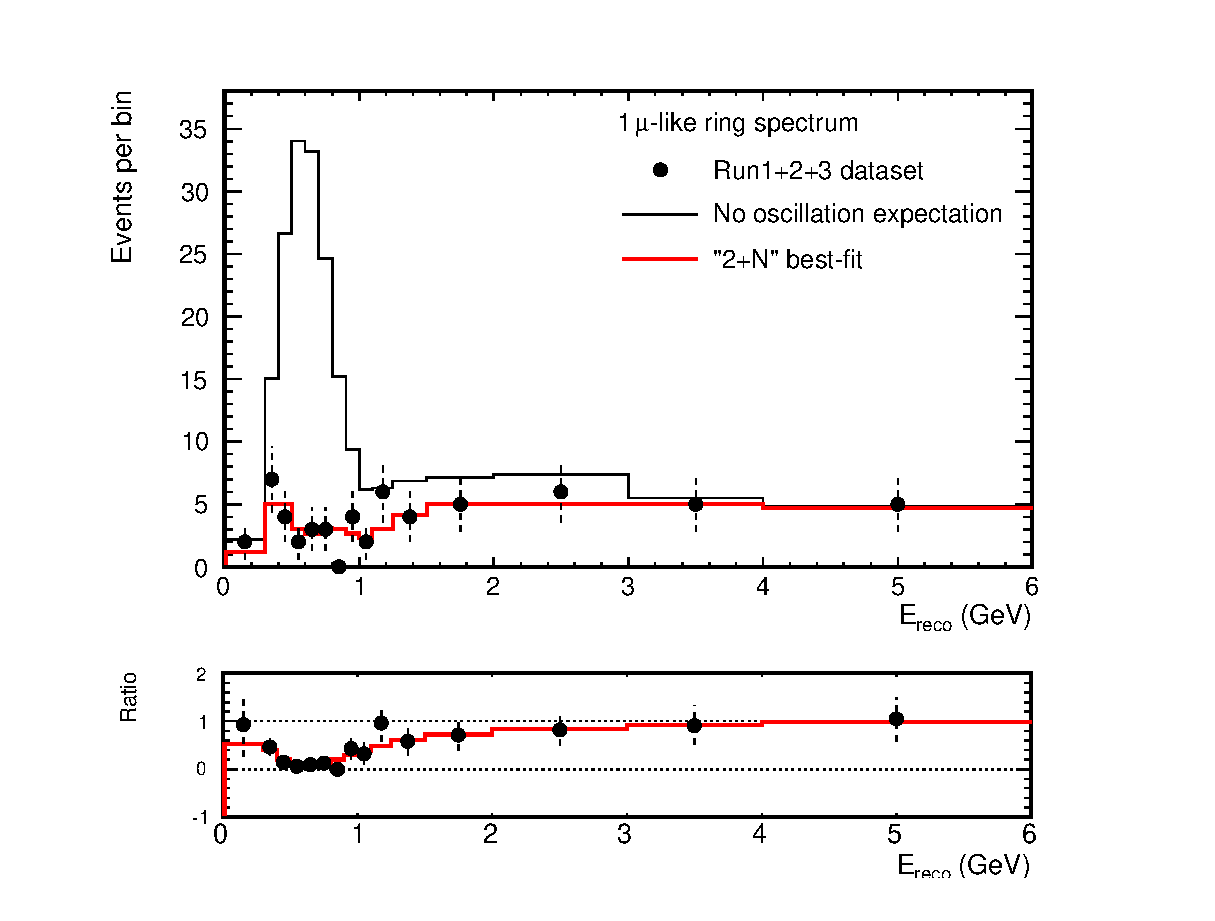
\includegraphics[width=34pc]{./images/fit_data/2N/spectrum_and_ratio_2N_coarse.eps}
\caption {
  Best-fit reconstructed energy spectrum using the coarse binning scheme (see 
  Sec.\ \ref{sec:results_bestfit_spectra}) obtained from the `2+N' fit to the Run 1+2+3 dataset.
  Also shown are the spectrum obtained under the no-oscillation hypothesis
  and the ratios of the data and best-fit spectrum to it.
}
\label{fig:results_data123_spectrum_coarse_2N}
\end{figure*}

\begin{figure*}[htb]
\center
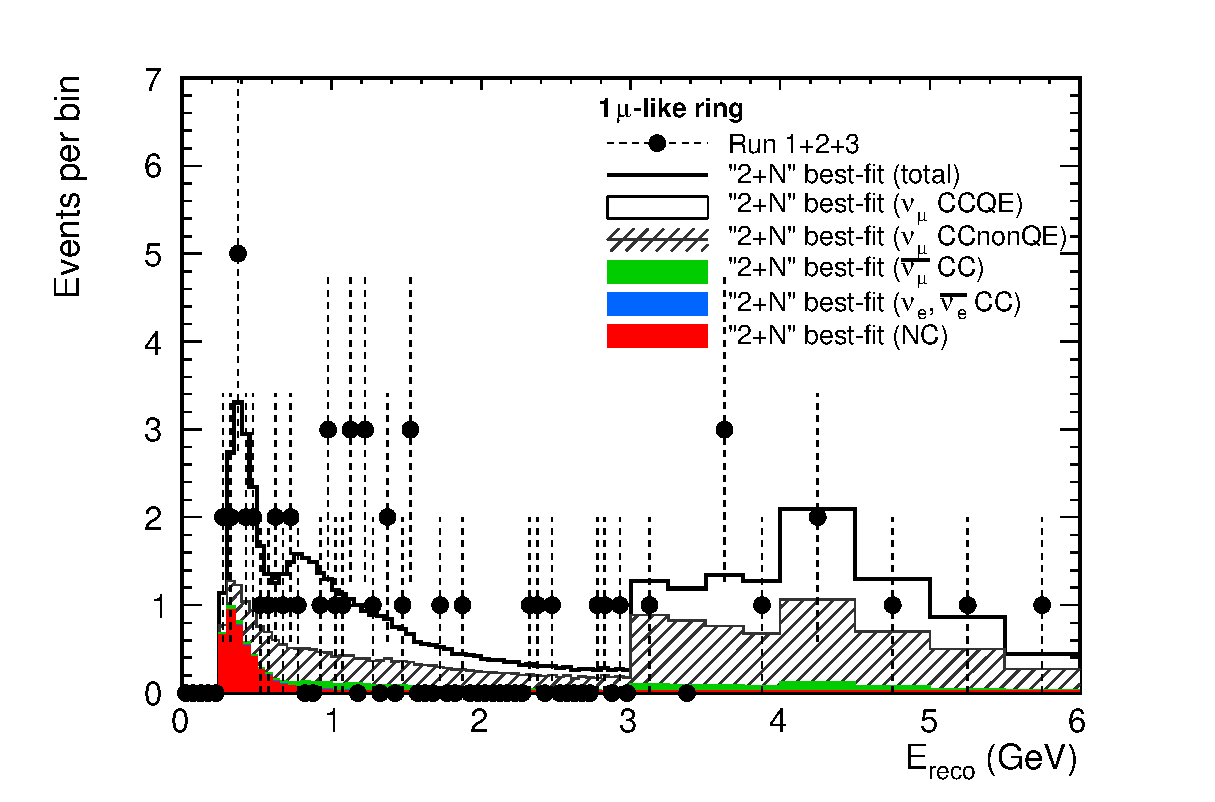
\includegraphics[width=24pc]{./images/fit_data/2N/bestfit_spectrum_with_modes_run123_2N.eps}
\caption {
  Best-fit reconstructed energy spectrum in the 73-bin scheme used in the fit (see 
  Sec.\ \ref{sec:mc_templates:template_binning}) and its components
  obtained from the `2+N' fit to the Run 1+2+3 dataset.  
  The 28 components, each of which is calculated separately, are grouped into just 5 categories:
  $\nu_{\mu}$ CCQE, $\nu_{\mu}$ CCnQE, $\bar{\nu_{\mu}}$ CC, $\nu_{e}$/$\bar{\nu_{e}}$ CC and NC.  
}
\label{fig:results_data123_spectrum_components_2N}
\end{figure*}

%...........................................................
%
% Best-fit spectra (total and components) and ratios for `2+N' fit in the second octant
% (Run1+2+3 only, coarse binning)
%

\begin{figure*}[htb]
\center
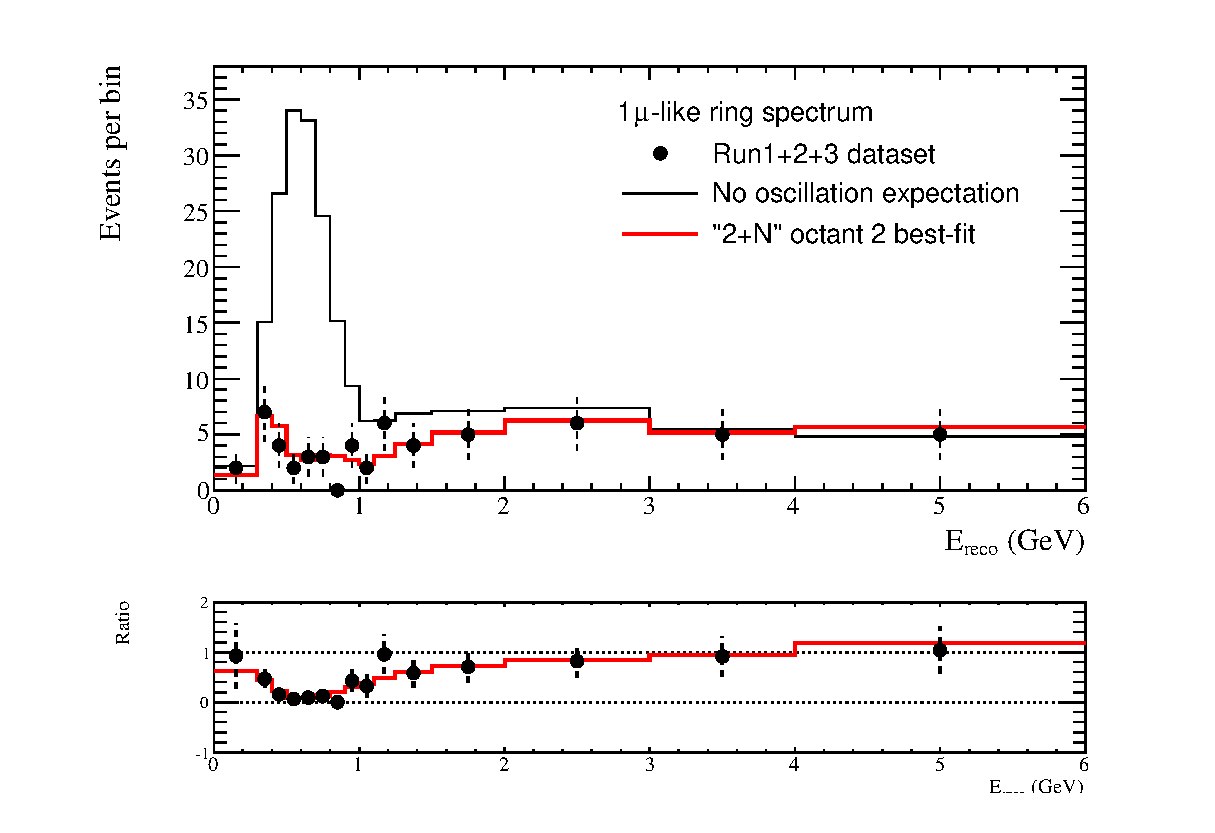
\includegraphics[width=34pc]{./images/fit_data/2Noctant2/spectrum_and_ratio_2N_coarse.eps}
\caption {
  Best-fit reconstructed energy spectrum using the coarse binning scheme (see 
  Sec.\ \ref{sec:results_bestfit_spectra}) obtained from the `2+N' fit to the Run 1+2+3 dataset,
  assuming $\theta_{23}$ is in the second octant.
  Also shown are the spectrum obtained under the no-oscillation hypothesis
  and the ratios of the data and best-fit spectrum to it.
}
\label{fig:results_data123_spectrum_coarse_2NO2}
\end{figure*}

\begin{figure*}[htb]
\center
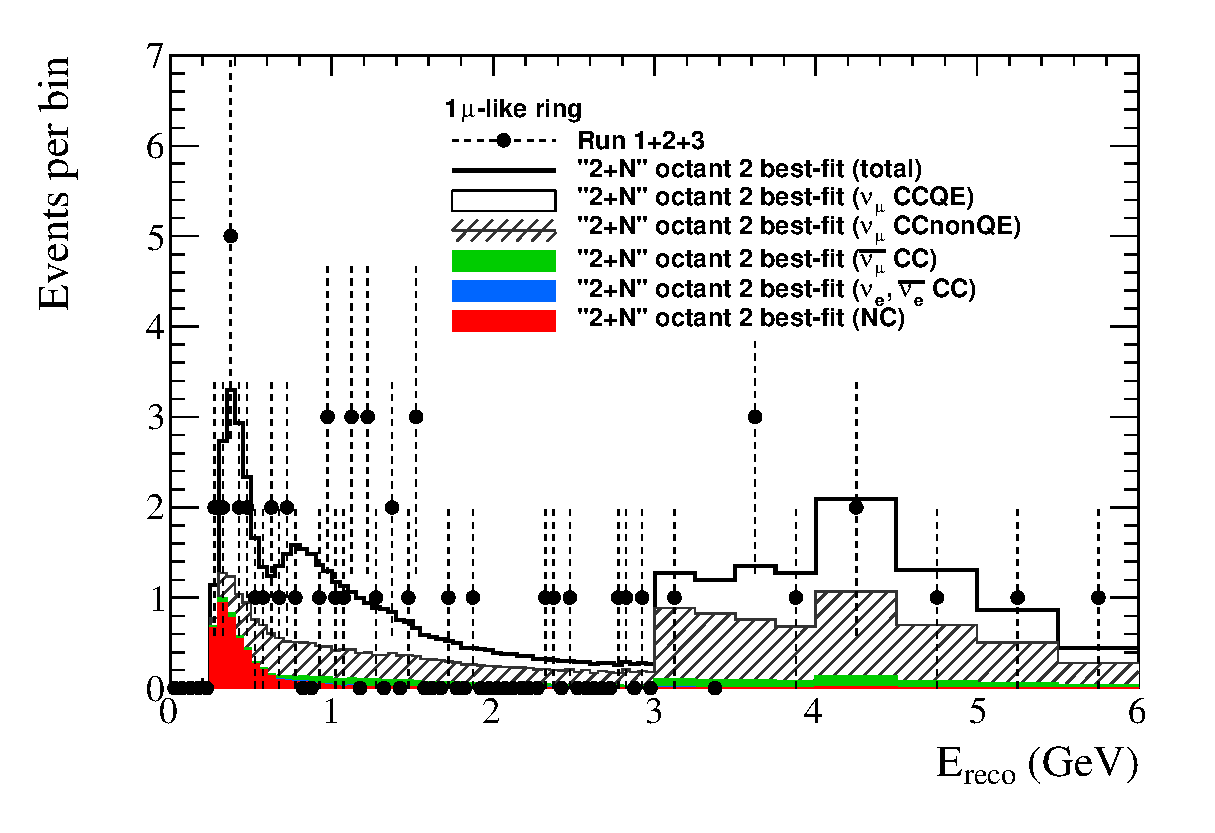
\includegraphics[width=24pc]{./images/fit_data/2Noctant2/bestfit_spectrum_with_modes_run123_2N.eps}
\caption {
  Best-fit reconstructed energy spectrum in the 73-bin scheme used in the fit (see 
  Sec.\ \ref{sec:mc_templates:template_binning}) and its components
  obtained from the `2+N' fit to the Run 1+2+3 dataset,
  assuming $\theta_{23}$ is in the the second octant.
  The 28 components, each of which is calculated separately, are grouped into just 5 categories:
  $\nu_{\mu}$ CCQE, $\nu_{\mu}$ CCnQE, $\bar{\nu_{\mu}}$ CC, $\nu_{e}$/$\bar{\nu_{e}}$ CC and NC.  
}
\label{fig:results_data123_spectrum_components_2NO2}
\end{figure*}

%...........................................................
%
% Best-fit spectra (total and components) and ratios for `2+8' fit 
% (Run1+2+3 only, coarse binning)
%

\begin{figure*}[htb]
\center
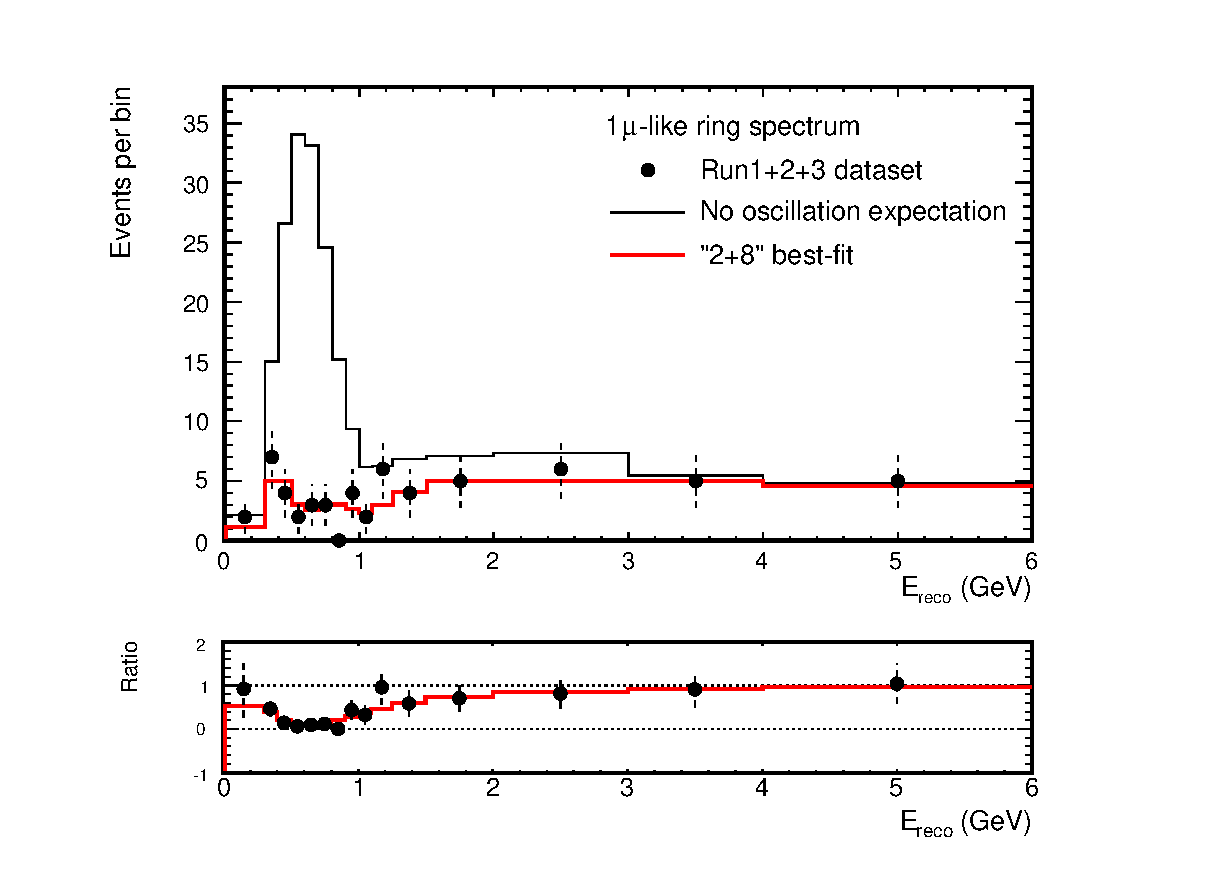
\includegraphics[width=34pc]{./images/fit_data/28/spectrum_and_ratio_28_coarse.eps}
\caption {
  Best-fit reconstructed energy spectrum using the coarse binning scheme (see 
  Sec.\ \ref{sec:results_bestfit_spectra})
  obtained from the `2+8' fit to the Run 1+2+3 dataset.
  Also shown are the spectrum obtained under the no-oscillation hypothesis
  and the ratios of the data and best-fit spectrum to it.
}
\label{fig:results_data123_spectrum_coarse}
\end{figure*}

\begin{figure*}[htb]
\center
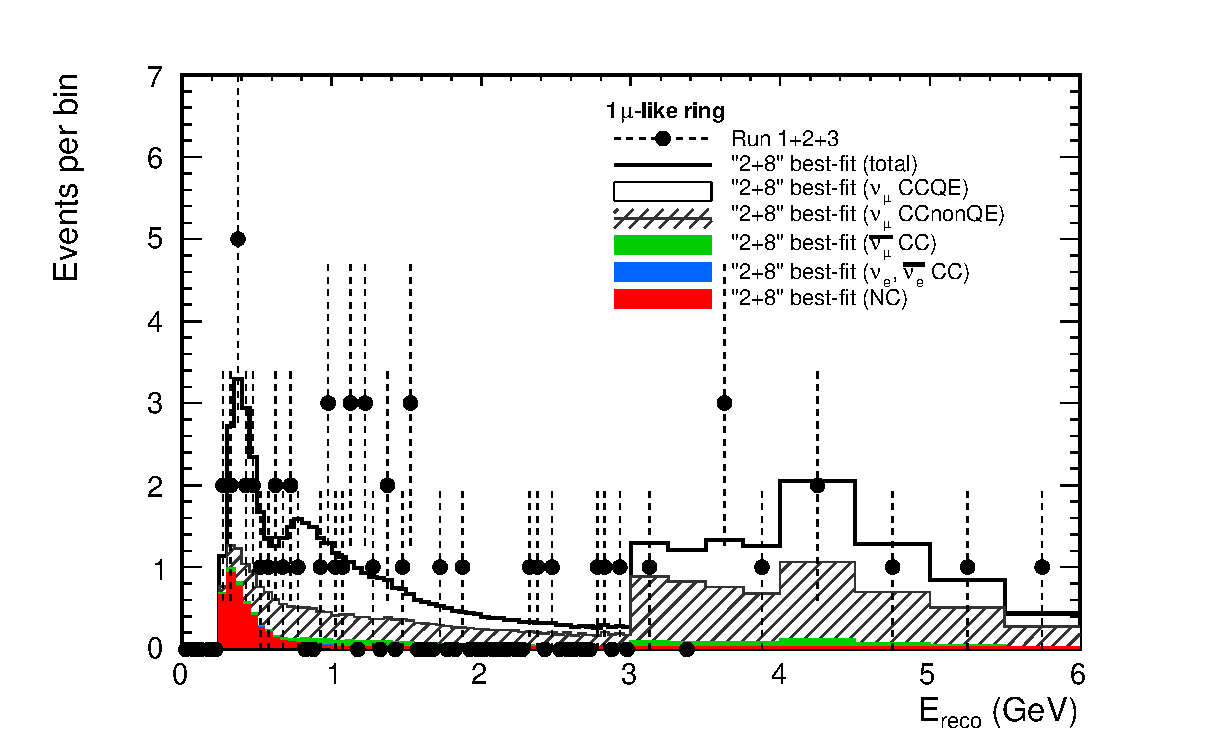
\includegraphics[width=24pc]{./images/fit_data/28/bestfit_spectrum_with_modes_run123_28.eps}
\caption {
  Best-fit reconstructed energy spectrum in the 73-bin scheme used in the fit (see
  Sec.\ \ref{sec:mc_templates:template_binning}) and its components
  obtained from the `2+8' fit to the Run 1+2+3 dataset.
  The 28 components, each of which is calculated separately, are grouped into just 5 categories:
  $\nu_{\mu}$ CCQE, $\nu_{\mu}$ CCnQE, $\bar{\nu_{\mu}}$ CC, $\nu_{e}$/$\bar{\nu_{e}}$ CC and NC.
}
\label{fig:results_data123_spectrum_components}
\end{figure*}

\clearpage
%...........................................................
%
% Comparison of `2+N' sintheta & second octant best-fit spectra and difference
% (Run1+2+3 only, 73 bins)
%

\begin{figure*}[htb]
\center
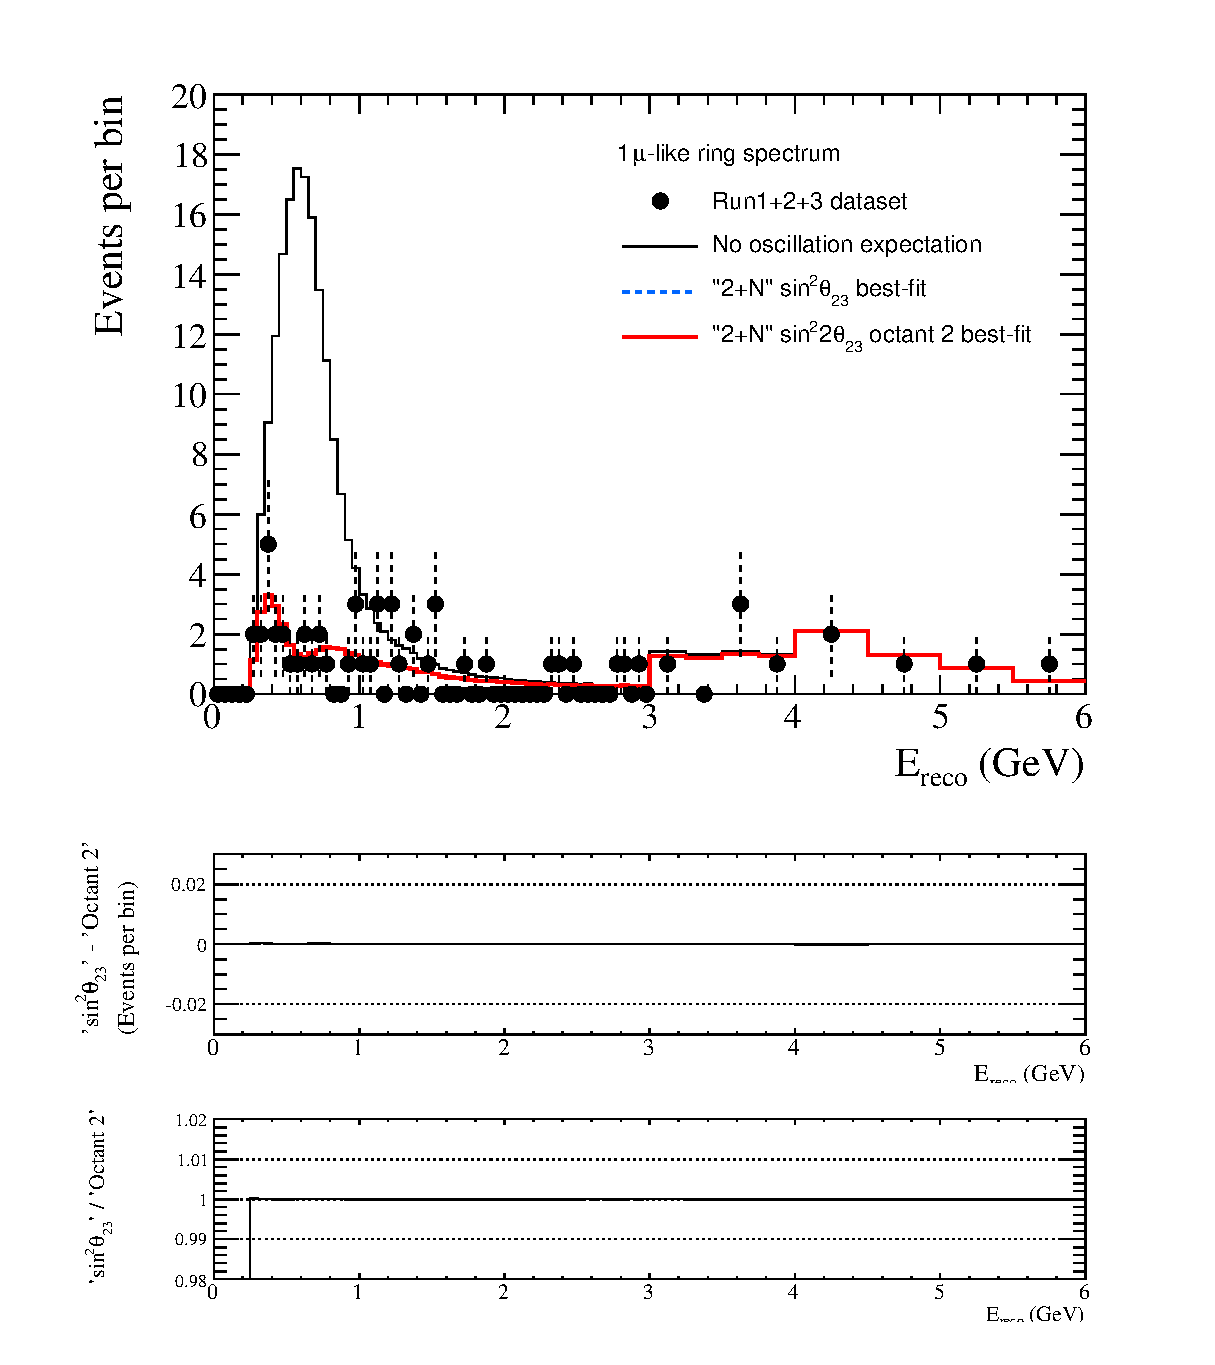
\includegraphics[width=40pc]{./images/fit_data/compare/spectrum_comparison_2Nsintheta_2NO2}
\caption {
  Comparison between best-fit reconstructed energy spectra
  obtained from the `2+N' fits to the Run 1+2+3 datasets, for
  the $\sin^2\theta_{23}$ fit, and the $\sin^2(2\theta_{23})$ fit assuming the second octant.
  The spectra are shown using the 73 bins used in the fit (see Sec.\ \ref{sec:mc_templates:template_binning}).
  Also shown are the absolute difference between the '$\sin^2\theta_{23}$' and '$\sin^2(2\theta_{23})$ octant 2' best-fit spectra and 
  the ratio between them.
}
\label{fig:results_data123_spectrum_comparison_sintheta}
\end{figure*}

%...........................................................
%
% Comparison of `2+N' sintheta & second octant best-fit spectra and fractional difference
% (Run1+2+3 only, coarser binning)
%

\begin{figure*}[htb]
\center
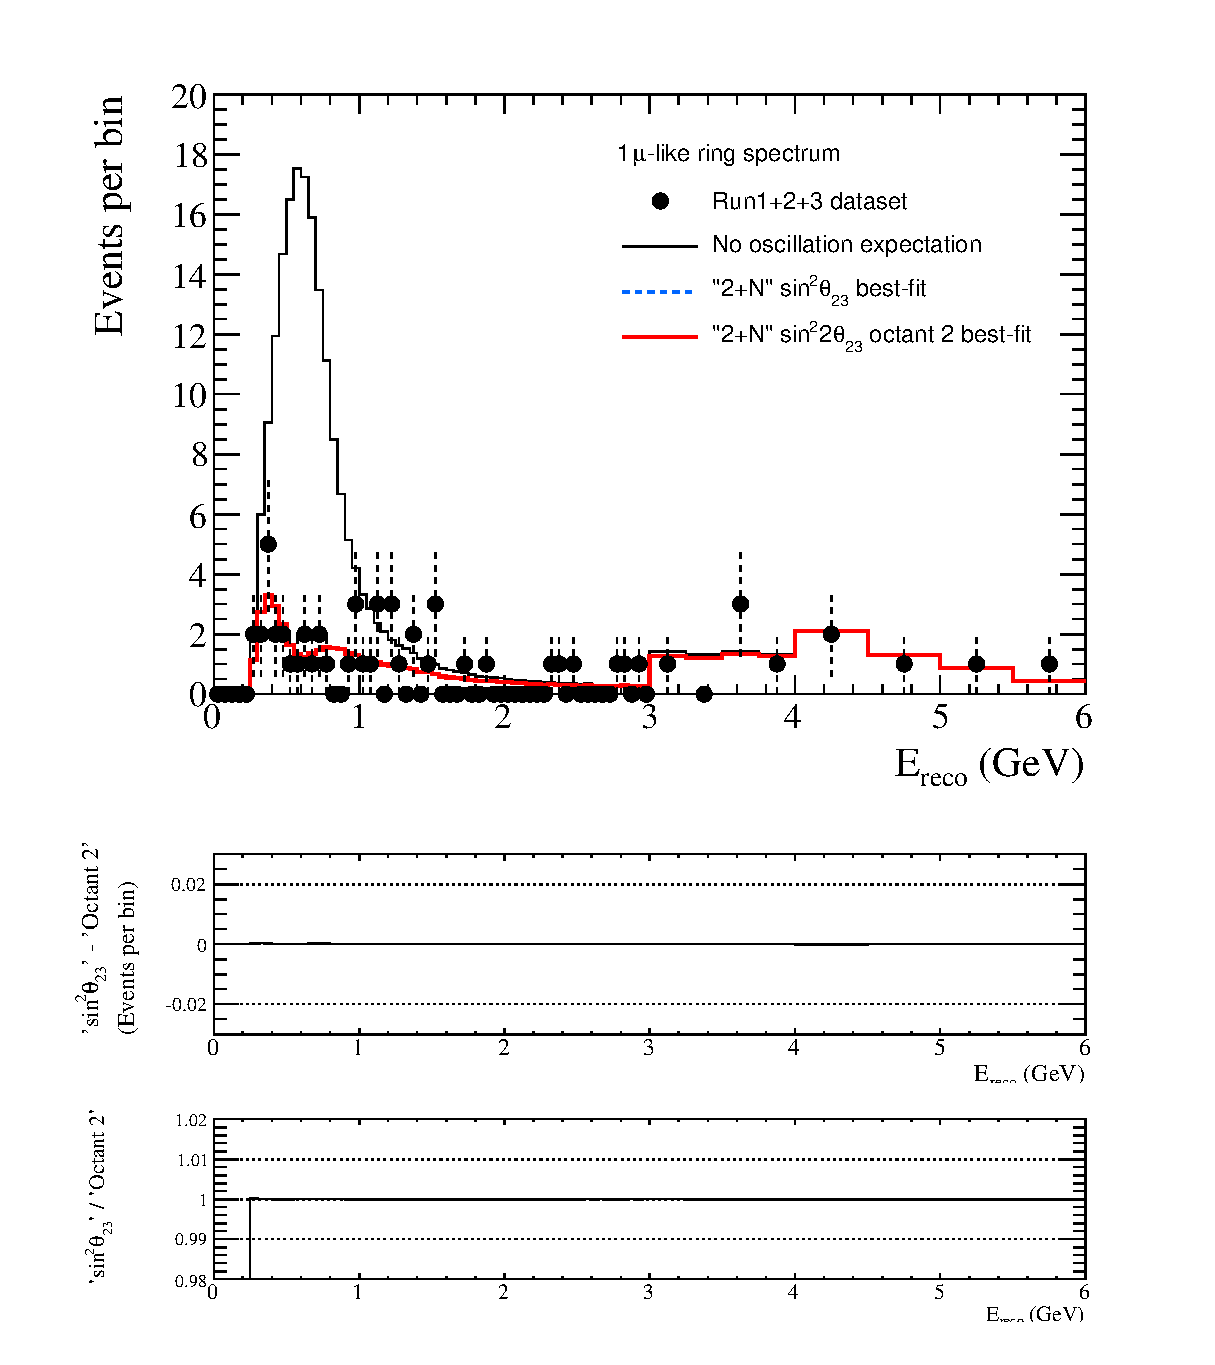
\includegraphics[width=40pc]{./images/fit_data/compare/spectrum_comparison_2Nsintheta_2NO2_coarse.eps}
\caption {
  Comparison between best-fit reconstructed energy spectra
  obtained from the `2+N' fits to the Run 1+2+3 datasets, for
  the $\sin^2\theta_{23}$ fit, and the $\sin^2(2\theta_{23})$ fit assuming the second octant.
  scheme (see Sec.\ \ref{sec:results_bestfit_spectra}).
  Also shown are the absolute difference between the '$\sin^2\theta_{23}$' and '$\sin^2(2\theta_{23})$ octant 2' best-fit spectra and 
  the ratio between them.
}
\label{fig:results_data123_spectrum_comparison_sintheta_coarse}
\end{figure*}


%...........................................................
%
% Comparison of `2+N' first & second octant best-fit spectra and difference
% (Run1+2+3 only, 73 bins)
%

\begin{figure*}[htb]
\center
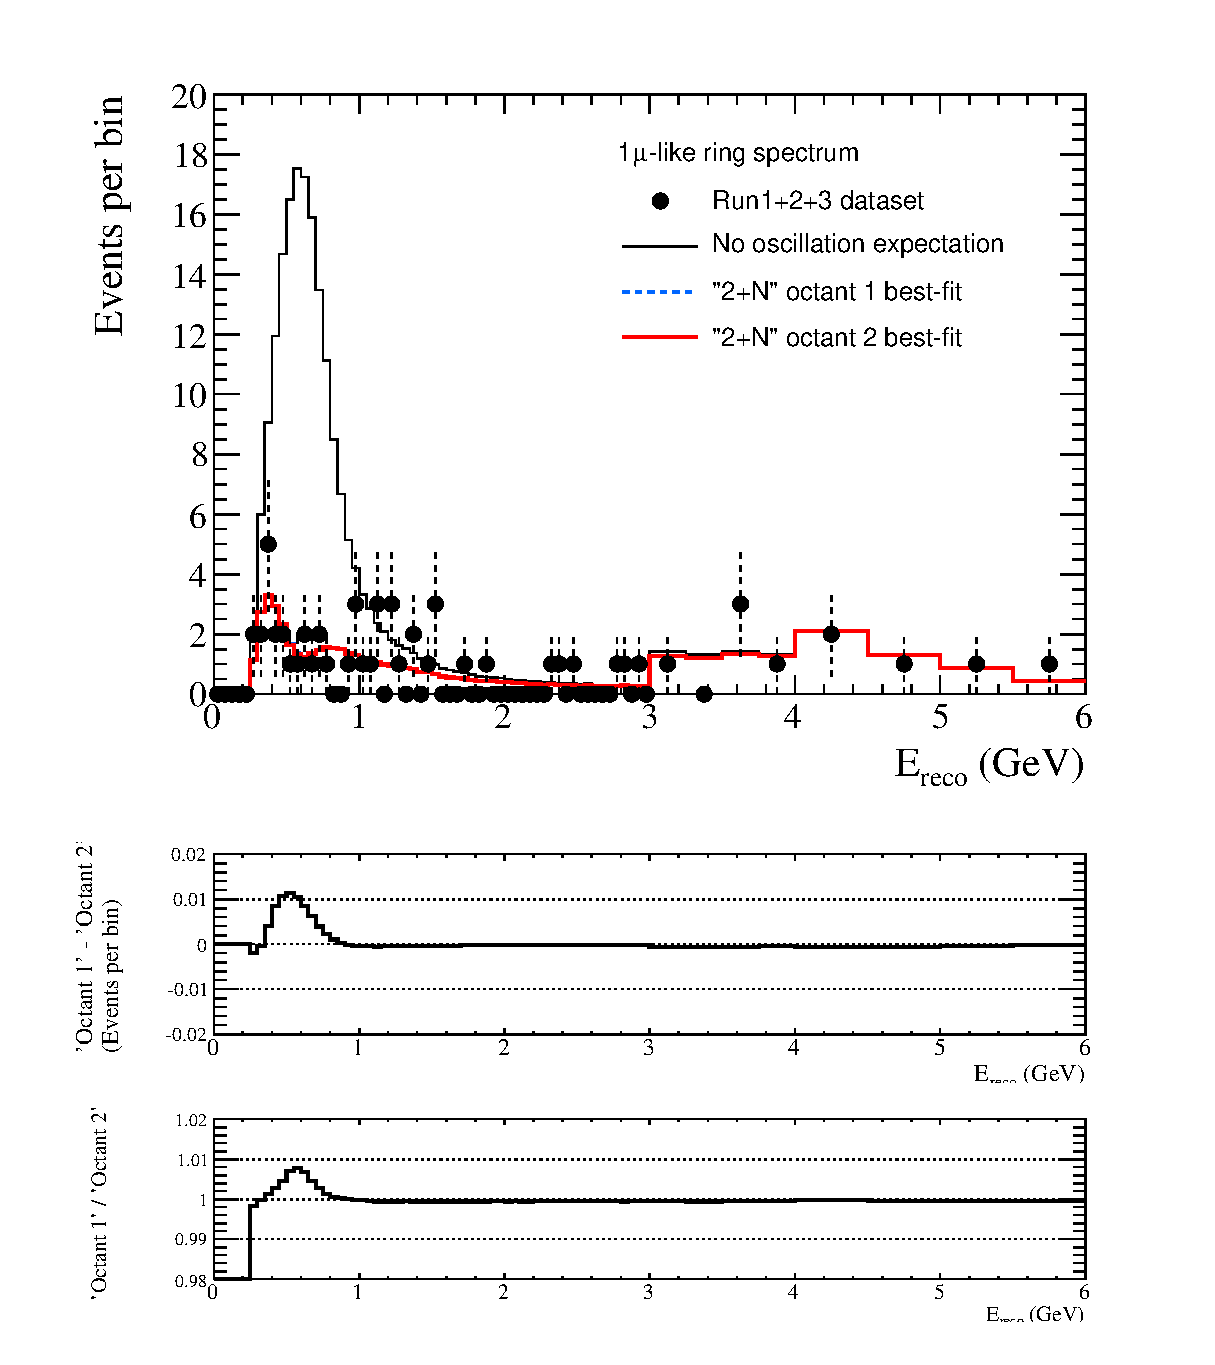
\includegraphics[width=40pc]{./images/fit_data/compare/spectrum_comparison_2N_2NO2}
\caption {
  Comparison between best-fit reconstructed energy spectra
  obtained from the `2+N' fits to the Run 1+2+3 datasets, for both $\theta_{23}$ octant assumptions.
  The spectra are shown using the 73 bins used in the fit (see Sec.\ \ref{sec:mc_templates:template_binning}).
  Also shown are the absolute difference between the '$\theta_{23}$ octant 1' and '$\theta_{23}$ octant 2' best-fit spectra and 
  the ratio between them.
}
\label{fig:results_data123_spectrum_comparison_octant}
\end{figure*}

%...........................................................
%
% Comparison of `2+N' first & second octant best-fit spectra and fractional difference
% (Run1+2+3 only, coarser binning)
%

\begin{figure*}[htb]
\center
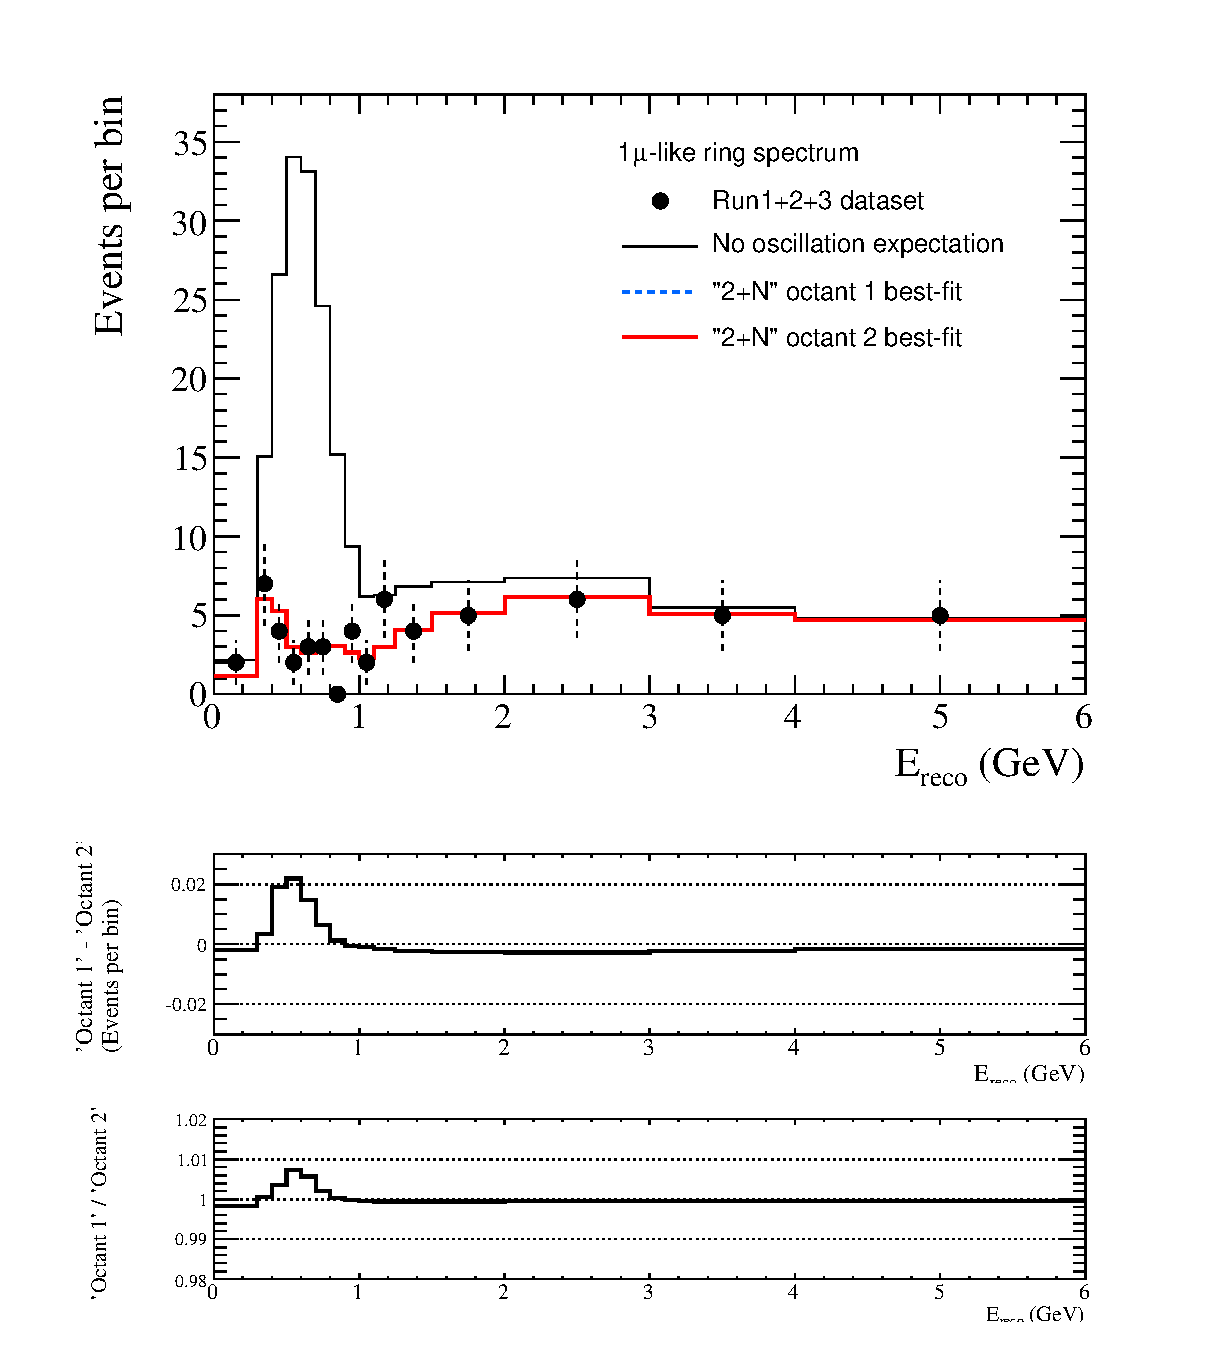
\includegraphics[width=40pc]{./images/fit_data/compare/spectrum_comparison_2N_2NO2_coarse.eps}
\caption {
  Comparison between best-fit reconstructed energy spectra
  obtained from the `2+N' fits to the Run 1+2+3 datasets, for both $\theta_{23}$ octant assumptions,
  using the coarse binning 
  scheme (see Sec.\ \ref{sec:results_bestfit_spectra}).
  Also shown are the absolute difference between the '$\theta_{23}$ octant 1' and '$\theta_{23}$ octant 2' best-fit spectra and
  the ratio between them.
}
\label{fig:results_data123_spectrum_comparison_octant_coarse}
\end{figure*}


%...........................................................
%
% Comparison of `2+N' and `2+8' best-fit spectra and difference
% (Run1+2+3 only, 73 bins)
%

\begin{figure*}[htb]
\center
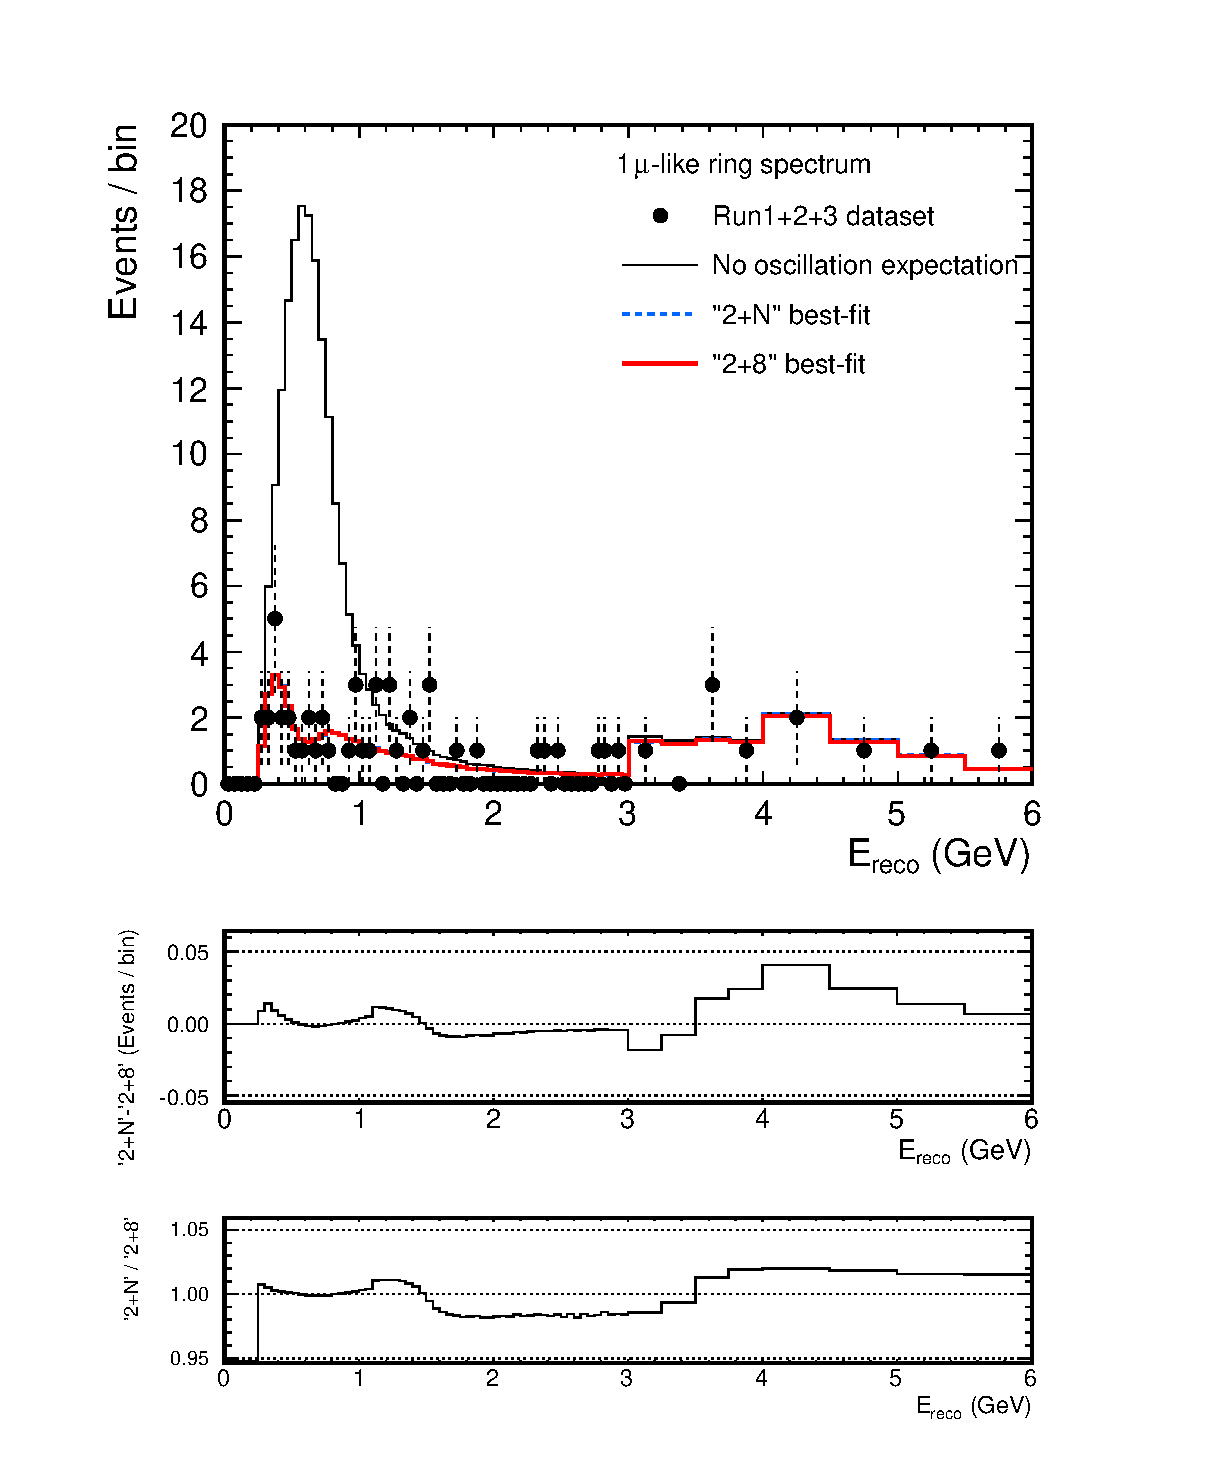
\includegraphics[width=40pc]{./images/fit_data/compare/spectrum_comparison_28_2N.eps}
\caption {
  Comparison between best-fit reconstructed energy spectra
  obtained from the `2+N' and `2+8' fits to the Run 1+2+3 datasets.
  The spectra are shown using the 73 bins used in the fit (see Sec.\ \ref{sec:mc_templates:template_binning}).
  Also shown are the absolute difference between the '2+N' and '2+8' best-fit spectra and 
  the ratio between them.
}
\label{fig:results_data123_spectrum_comparison}
\end{figure*}

%...........................................................
%
% Comparison of `2+N' and `2+8' best-fit spectra and fractional difference
% (Run1+2+3 only, coarser binning)
%

\begin{figure*}[htb]
\center
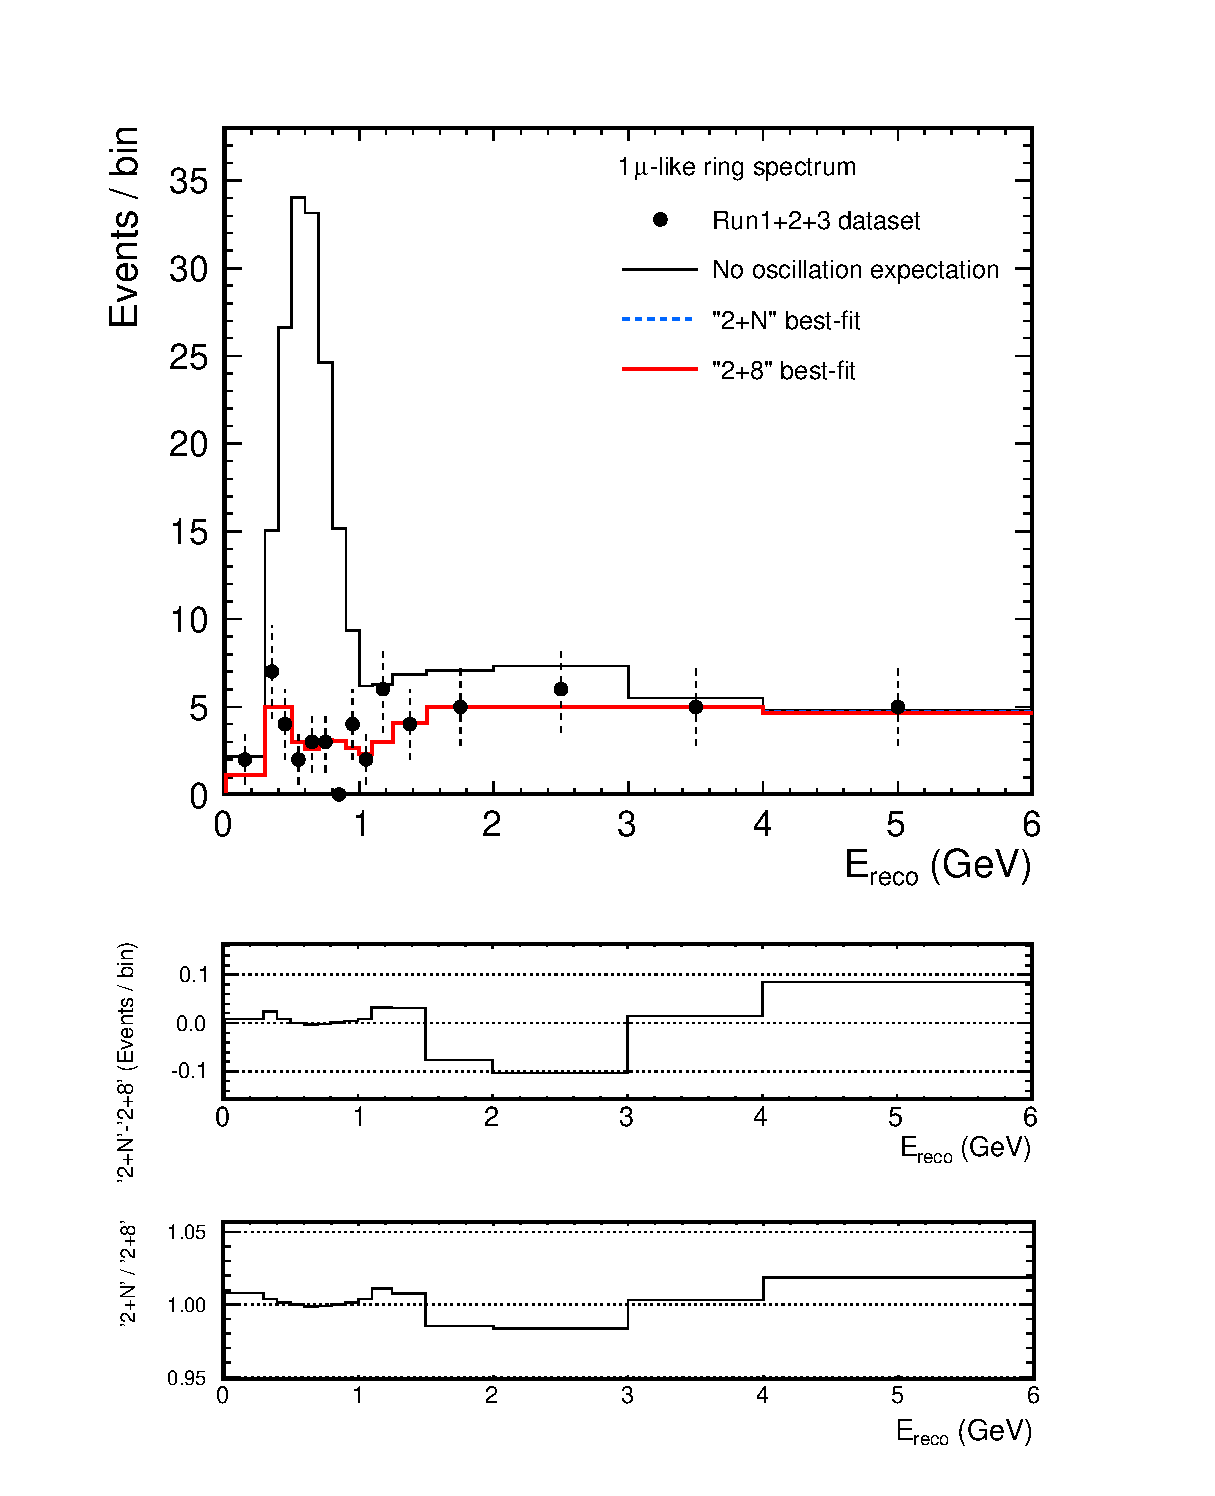
\includegraphics[width=40pc]{./images/fit_data/compare/spectrum_comparison_28_2N_coarse.eps}
\caption {
  Comparison between best-fit reconstructed energy spectra
  obtained from the `2+N' and `2+8' fits to the Run 1+2+3 datasets using the coarse binning 
  scheme (see Sec.\ \ref{sec:results_bestfit_spectra}).
  Also shown are the absolute difference between the '2+N' and '2+8' best-fit spectra and
  the ratio between them.
}
\label{fig:results_data123_spectrum_comparison_coarse}
\end{figure*}


%--------------------------------------------------------------------------------------
% Limits
%--------------------------------------------------------------------------------------

\clearpage

\subsection {Confidence limits}
\label{sec:results_limits}

The first step in calculating confidence limits for a single oscillation
parameter is to calculate the values of $\Delta\chi^2$ for each value of that oscillation 
parameter. For each value of $\sin^{2}2\theta_{23}$, a `1+N' fit is done with $|\Delta m^{2}_{32}|$ 
and all the systematic parameters allowed to float and $\sin^{2}2\theta_{23}$ fixed. Then 
$\Delta\chi^2$ is calculated for that value of $\sin^{2}2\theta_{23}$ by subtracting 
the `2+N' best-fit value of $\chi^2$ over the whole 2D oscillation parameter grid 
(which is listed in Tab.\ \ref{tab:data_fits:best_fit_values}). The 68\% and 90\% 
confidence intervals in $\sin^{2}2\theta_{23}$ are found using the constant-$\Delta\chi^2$ method, 
as described in Sec.\ \ref{sec:contour_construction_constdchi}, and are given by the values for 
which $\chi^2$ increases from the minimum by 1.00 and 2.71 respectively. Then this procedure 
is repeated for $|\Delta m^{2}_{32}|$\footnote{
  The procedure is equivalent for the limits with $\sin^2\theta_{23}$,
  just with a different fit parameter.
}.

The constant-$\Delta \chi^{2}$ method is used for the 1D confidence
limits since there is a problem in using the Feldman-Cousins
method. There is no obvious way of choosing the true value(s) of
$|\Delta m_{32}^{2}|$ as inputs to the toy MC experiments to find the
critical values of $\Delta \chi^{2}$ for the 1D confidence interval in
$\sin^{2} 2\theta_{23}$. The same difficulty arises when choosing the
true values of $\sin^{2} 2\theta_{23}$ to find the critical values of
$\Delta \chi^{2}$ for the 1D confidence interval in $|\Delta
m_{32}^{2}|$.

The $\Delta\chi^2$ distributions for $\sin^{2}\theta_{23}$ and $|\Delta m^{2}_{32}|$ for the 
`1+N' fit to the Run 1+2+3 dataset are shown in Figs.\
\ref{fig:results_data123_1dcontour_mixing23_sintheta} and
\ref{fig:results_data123_1dcontour_dm23sq_sintheta} respectively, along with the
68\% and 90\% constant-$\Delta\chi^2$ critical values.
These provide the 68\% errors $\sin^{2}\theta_{23} = 0.514\pm0.082$
and $|\Delta m^2_{32}| = 2.44^{+0.17}_{-0.15}$$\times$10$^{-3}$ eV$^{2}$/c$^{4}$,
and the limits of
$0.397 < \sin^{2}\theta_{23} < 0.630$
and
$2.19$$\times$10$^{-3}$ eV$^{2}$/c$^{4}$ $< |\Delta m^2_{32}| < 2.72$$\times$10$^{-3}$ eV$^{2}$/c$^{4}$
at 90\% C.L.

The $\Delta\chi^2$ distributions for $\sin^{2}2\theta_{23}$ and $|\Delta m^{2}_{32}|$ for the 
`1+N' fit to the Run 1+2+3 dataset are shown in Figs.\
\ref{fig:results_data123_1dcontour_mixing23} and
\ref{fig:results_data123_1dcontour_dm23sq} respectively, along with the
68\% and 90\% constant-$\Delta\chi^2$ critical values.
Results are shown for $\theta_{23}$ in both the first and second octants.
For the first octant, these provide the 68\% errors $\sin^{2}2\theta_{23} = 1.000^{+0.000}_{-0.019}$
and $|\Delta m^2_{32}| = 2.44^{+0.17}_{-0.15}$$\times$10$^{-3}$ eV$^{2}$/c$^{4}$,
and the limits of $\sin^{2}2\theta_{23}$ $>$ 0.958 and
$2.19$$\times$10$^{-3}$ eV$^{2}$/c$^{4}$ $< |\Delta m^2_{32}| < 2.72$$\times$10$^{-3}$ eV$^{2}$/c$^{4}$
at 90\% C.L. 
For the second octant, these provide the 68\% errors $\sin^{2}2\theta_{23} = 0.999^{+0.001}_{-0.036}$
and $|\Delta m^2_{32}| = 2.44^{+0.17}_{-0.15}$$\times$10$^{-3}$ eV$^{2}$/c$^{4}$,
and the limits of $\sin^{2}2\theta_{23}$ $>$ 0.931 and
$2.19$$\times$10$^{-3}$ eV$^{2}$/c$^{4}$ $< |\Delta m^2_{32}| < 2.72$$\times$10$^{-3}$ eV$^{2}$/c$^{4}$
at 90\% C.L.
The 1D limits for the second octant are identical to those for the first octant for $|\Delta m^2_{32}|$,
but much wider for $\sin^{2}2\theta_{23}$.
This can be understood from Eq.\ \ref{eqn:numusurv3fapprox} since
the center of symmetry (point of maximal disappearance) is in the second octant.

%...........................................................
%
% sinsqtheta23 fit limits
%

\begin{figure*}[htb]
%\begin{minipage}[t]{0.90\linewidth}
\begin{minipage}[t]{0.48\linewidth}
\center
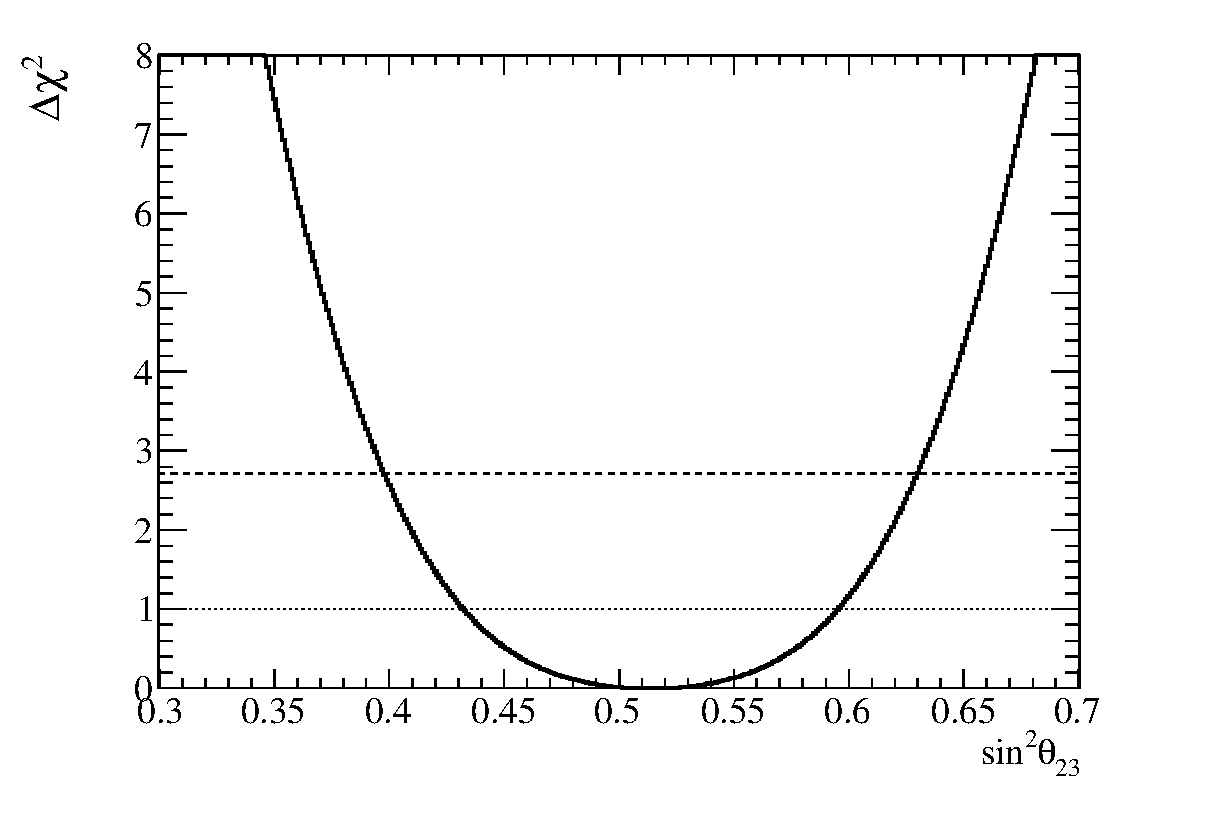
\includegraphics[width=20pc]{./images/fit_data/2Nsintheta/1D_contour_mixing23_lines}
\caption {$\Delta \chi^2$ as a function of $\sin^2\theta_{23}$
  for the `1+N' fit to the Run 1+2+3 dataset.
  The 68\% and 90\% constant-$\Delta\chi^2$ critical values are shown
  as dotted and dashed lines respectively.
}
\label{fig:results_data123_1dcontour_mixing23_sintheta}
\end{minipage}
%\vfill
\hspace{0.06\linewidth}
%\begin{minipage}[t]{0.90\linewidth}
\begin{minipage}[t]{0.48\linewidth}
\center
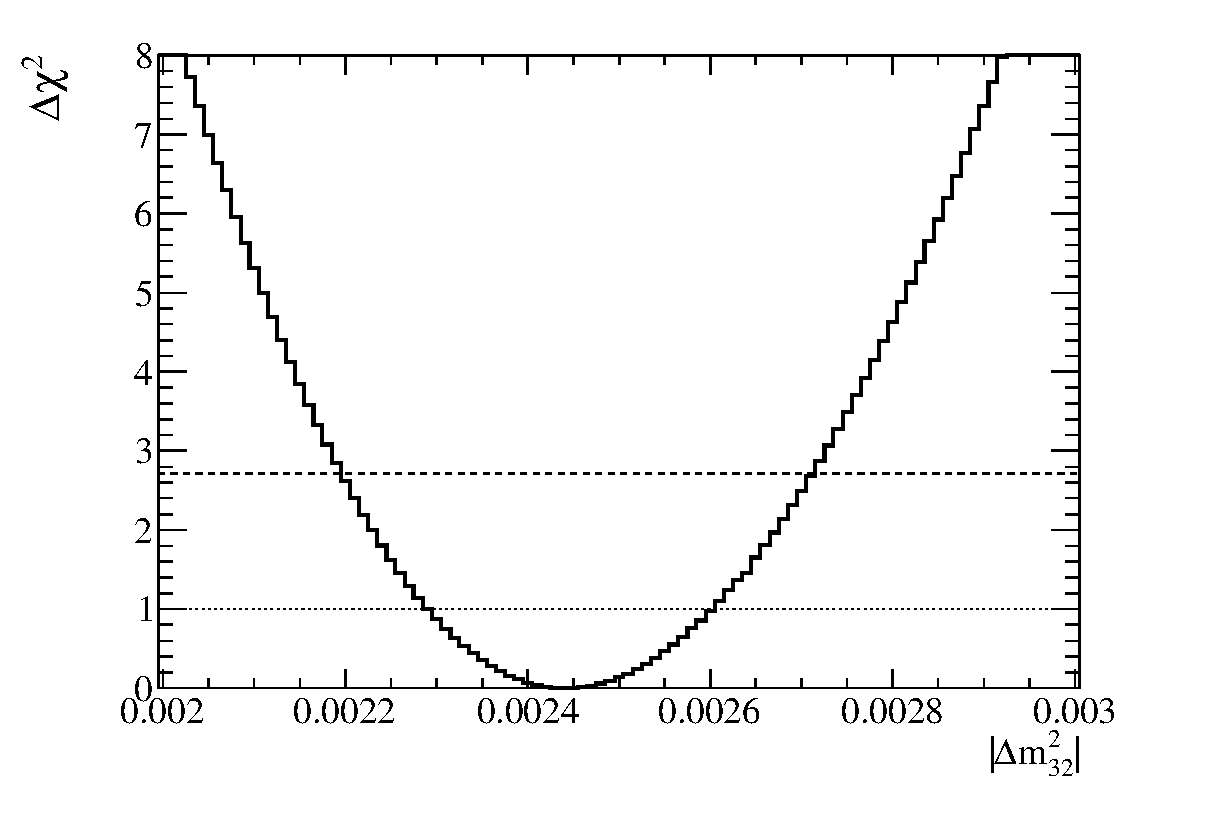
\includegraphics[width=20pc]{./images/fit_data/2Nsintheta/1D_contour_dm23sq_lines}
\caption { 
  $\Delta \chi^2$ as a function of $|\Delta m^{2}_{32}|$
  for the `1+N' fit to the Run 1+2+3 dataset.
  The 68\% and 90\% constant-$\Delta\chi^2$ critical values are shown
  as dotted and dashed lines respectively.
}
\label{fig:results_data123_1dcontour_dm23sq_sintheta}
\end{minipage}
\end{figure*}

%...........................................................
%
% sinsq2theta23 fit limits
%

\begin{figure*}[htb]
%\begin{minipage}[t]{0.90\linewidth}
\begin{minipage}[t]{0.48\linewidth}
\center
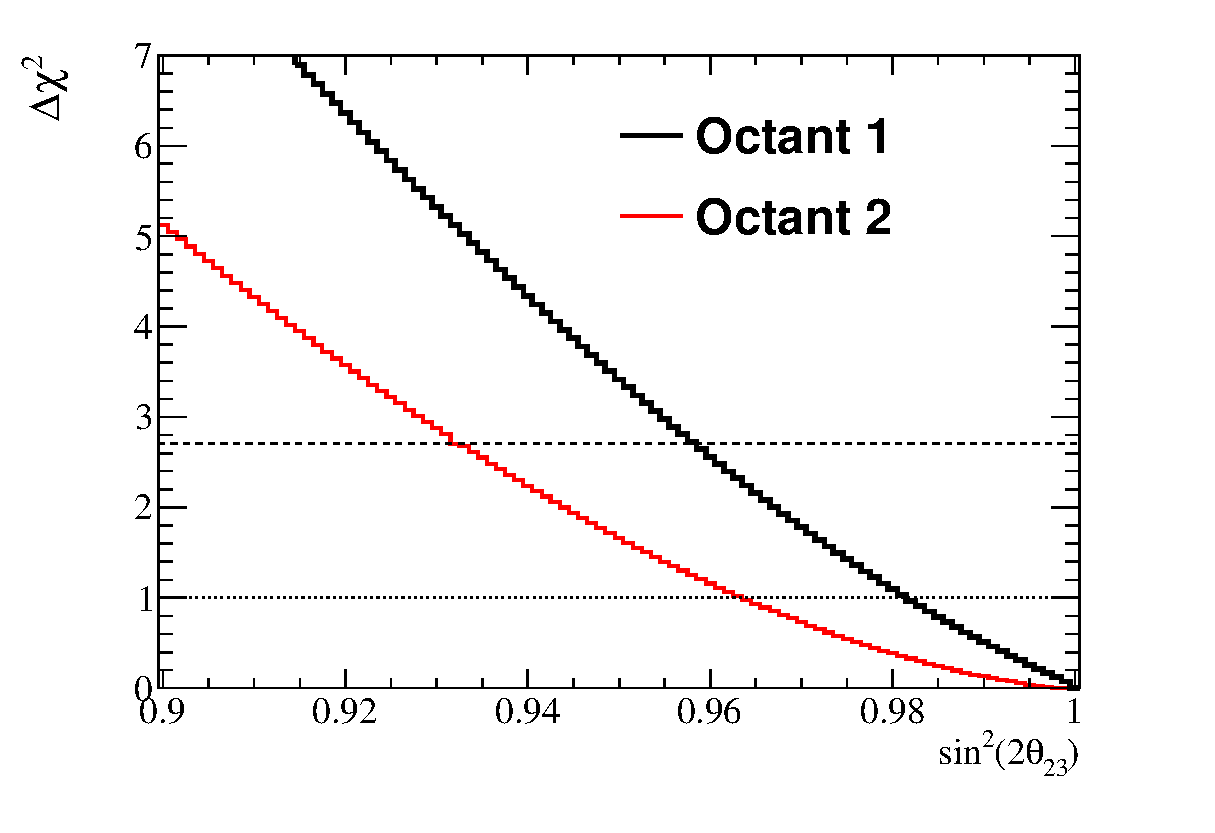
\includegraphics[width=20pc]{./images/fit_data/2N/1D_contour_mixing23_lines}
\caption {$\Delta \chi^2$ as a function of $\sin^22\theta_{23}$
  for the `1+N' fit to the Run 1+2+3 dataset.
  Results are shown for $\theta_{23}$ in for both octants.
  The 68\% and 90\% constant-$\Delta\chi^2$ critical values are shown
  as dotted and dashed lines respectively.
}
\label{fig:results_data123_1dcontour_mixing23}
\end{minipage}
%\vfill
\hspace{0.06\linewidth}
%\begin{minipage}[t]{0.90\linewidth}
\begin{minipage}[t]{0.48\linewidth}
\center
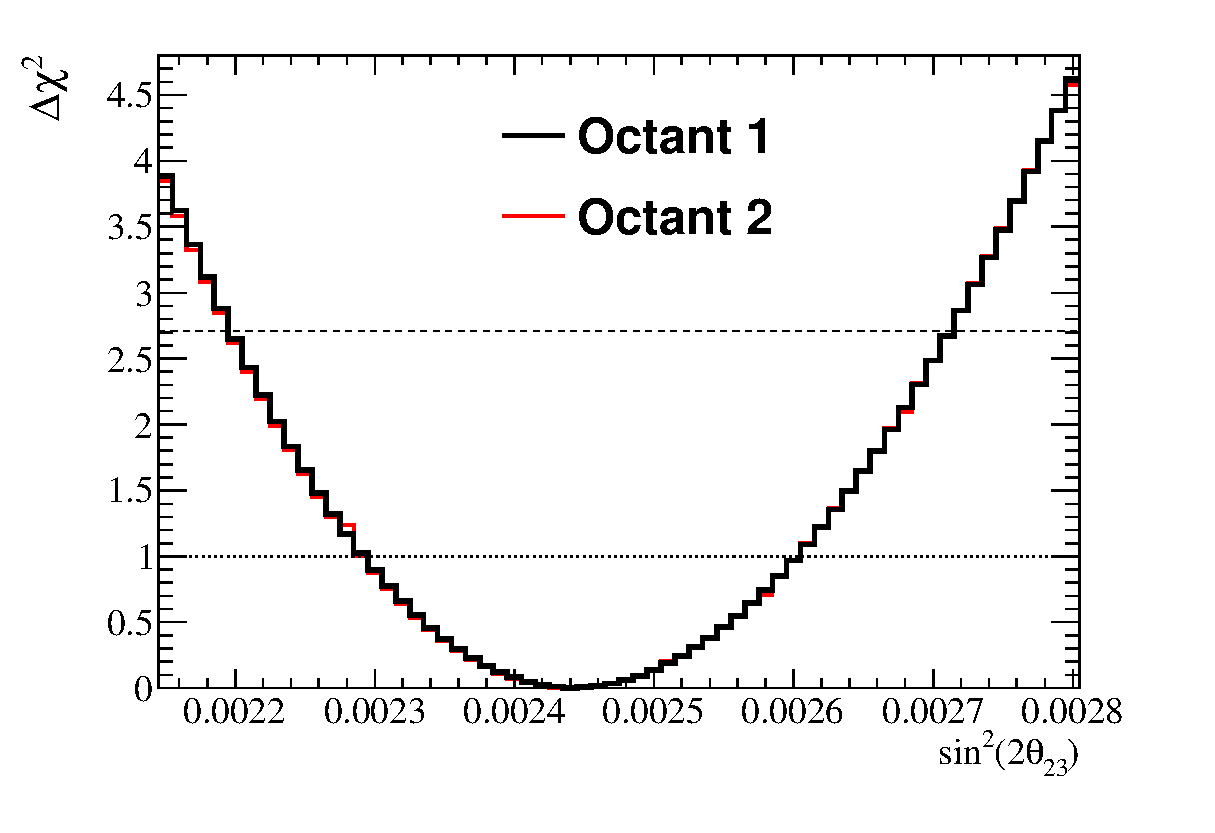
\includegraphics[width=20pc]{./images/fit_data/2N/1D_contour_dm23sq_lines}
\caption { 
  $\Delta \chi^2$ as a function of $|\Delta m^{2}_{32}|$
  for the `1+N' fit to the Run 1+2+3 dataset.
  Results are shown for $\theta_{23}$ in both octants.
  The 68\% and 90\% constant-$\Delta\chi^2$ critical values are shown
  as dotted and dashed lines respectively.
}
\label{fig:results_data123_1dcontour_dm23sq}
\end{minipage}
\end{figure*}


%--------------------------------------------------------------------------------------
% Contours
%--------------------------------------------------------------------------------------

\clearpage

\subsection {Confidence regions}
\label{sec:results_contours}

The first step in constructing confidence contours in the oscillation parameters $\sin^{2}2\theta_{23}$ 
and $|\Delta m^{2}_{32}|$ is to calculate 
the values of $\Delta\chi^2$ for each point in a 2-dimensional grid in the oscillation parameter 
space. This is done as described in Sec.\ \ref{sec:contour_construction_constdchi} for the 
constant-$\Delta\chi^2$ method and in Sec.\ \ref{sec:contour_construction_fc} for the Feldman-Cousins method. 

The $\Delta\chi^2$ surface for the the `2+N' fit for $\sin^2\theta_{23}$ to the Run 1+2+3 dataset is shown in Fig.\
\ref{fig:results_data123_chisq_2Nsintheta}, 
as a function of $\sin^{2}\theta_{23}$ and $|\Delta m^{2}_{32}|$.

The $\Delta\chi^2$ surface for the the `2+N' fit
to the Run 1+2+3 dataset is shown in Figs.\
\ref{fig:results_data123_chisq_2N} and \ref{fig:results_data123_chisq_2NO2}
for $\theta_{23}$ in the first and second octants respectively,
as a function of $\sin^{2}2\theta_{23}$ and $|\Delta m^{2}_{32}|$.
For comparison, the corresponding $\Delta\chi^2$ surfaces for the `2+N' fits to the Run 1+2 and Run 3 
datasets are shown in 
Figs.\ \ref{fig:results_data12_chisq_2N} and \ref{fig:results_data3_chisq_2N} respectively.
The same $\Delta\chi^2$ range is used in all colour plots to allow comparison.
Marginalized $\Delta\chi^2$ distributions are also shown as a function of either $\sin^{2}2\theta_{23}$ 
or $|\Delta m^{2}_{32}|$ for the `2+N' fits to the Run 1+2+3, Run 1+2 and Run 3 datasets in Figs.\ 
\ref{fig:results_marg_dchisq_dmsq_all3_2N} and \ref{fig:results_marg_dchisq_sinsq_all3_2N}
respectively.

The corresponding plots for the `2+8' fits are shown in Fig.\ \ref{fig:results_data123_chisq} for the 
Run 1+2+3 datset, Fig.\ \ref{fig:results_data12_chisq} for the Run 1+2 dataset and Fig.\ 
\ref{fig:results_data3_chisq} for the Run 3 dataset. Meanwhile the marginalized $\Delta\chi^2$ distributions are 
shown for all the datasets as a function of $\sin^{2}2\theta_{23}$ in Fig.\ \ref{fig:results_marg_dchisq_sinsq_all3} 
and as a function of $|\Delta m^{2}_{32}|$ in Fig.\ \ref{fig:results_marg_dchisq_dmsq_all3}.

Comparisons were made between the `2+N' $\Delta\chi^2$ distributions for $\theta_{23}$ in the first and second octants.
The fractional difference between the $\Delta\chi^2$ surfaces
obtained from the `2+N' fits, assuming the first and second octant, to the Run 1+2+3 dataset is shown in 
Fig.\ \ref{fig:results_dchisq_fracdiff_run123_octant}.
% The marginalized $\Delta\chi^2$ distributions 
% for the `2+N' fits, assuming the first and second octant, to the Run 1+2+3 dataset are compared
% as a function of $|\Delta m^{2}_{32}|$ in Fig.\ \ref{fig:results_comp_marg_dchisq_dmsq_run123_octant}
% and as a function of $\sin^{2}2\theta_{23}$ in Fig.\ \ref{fig:results_comp_marg_dchisq_sinsq_run123_octant}. 

Comparisons were made between the `2+N' and `2+8' $\Delta\chi^2$ distributions.
The fractional difference between the $\Delta\chi^2$ surfaces
obtained from the `2+N' and `2+8' fits to the Run 1+2+3 dataset is shown in 
Fig.\ \ref{fig:results_dchisq_fracdiff_run123}. The marginalized $\Delta\chi^2$ distributions 
for the `2+N' and `2+8' fits to the Run 1+2+3 dataset are compared as a function of $|\Delta m^{2}_{32}|$ 
in Fig.\ \ref{fig:results_comp_marg_dchisq_dmsq_run123} and as a function of $\sin^{2}2\theta_{23}$ 
in Fig.\ \ref{fig:results_comp_marg_dchisq_sinsq_run123}. 
As shown in these figures, 
the `2+N' and `2+8' marginalized $\Delta\chi^2$ distributions are almost identical,
even  in areas of the parameter space that exceed the 99\% CL region 
($\Delta\chi^{2} < $ 6.63 for a single parameter).

Confidence regions were constructed using both the constant-$\Delta\chi^2$ method described in 
Sec.\ \ref{sec:contour_construction_constdchi} and the Feldman-Cousins method described in Sec.\ 
\ref{sec:contour_construction_fc} for both the `2+N' and the `2+8' fits. Confidence contours were 
drawn using the constant-$\Delta\chi^2$ method for each of the Run 1+2+3, Run 1+2 and Run 3 datasets. 
Using the Feldman-Cousins method, however, they were drawn only for the Run 1+2+3 dataset 
due to the large amount of CPU time needed.
All confidence regions presented below include the effect of systematic uncertainties.

The 68\% and 90\% CL regions for the `2+N' $\sin^2\theta_{23}$ fit to the Run 1+2+3 dataset are shown using the constant-
$\Delta\chi^2$ method in Fig.\ \ref{fig:results_data123_contour_2Nsintheta}.
The corresponding constant-$\Delta\chi^2$ contours for the
Run 1+2+3 dataset (assuming $\theta_{23}$ is in the first octant),
the Run 1+2+3 dataset (assuming $\theta_{23}$ is in the second octant),
and the Run 1+2 and Run 3 datasets are shown 
in Figs.\ \ref{fig:results_data123_contour_2N}, \ref{fig:results_data123_contour_2NO2},
\ref{fig:results_data12_contour_2N} and \ref{fig:results_data3_contour_2N} respectively. 
The constant-$\Delta\chi^2$ contours for the '2+8' fits 
are shown in Fig.\ \ref{fig:results_data123_contour} for Run 1+2+3, 
in Fig.\ \ref{fig:results_data12_contour} 
for Run 1+2 and in Fig.\ \ref{fig:results_data3_contour} for Run 3.

The Feldman-Cousins 68\% and 90\% CL regions for the fits to the Run 1+2+3 dataset are shown 
in Fig.\ \ref{fig:results_data123_fc_contour_2N} for the `2+N' fit (assuming $\theta_{23}$ is in the first octant),
in Fig.\ \ref{fig:results_data123_fc_contour_2NO2} for the `2+N' fit (assuming $\theta_{23}$ is in the second octant), and
in Fig.\ \ref{fig:results_data123_fc_contour} for the `2+8' fit.
The boundary of the 68\% '2+N' contour assuming $\theta_{23}$ is in the first octant includes the points
($\sin^2(2\theta_{23})$,$|\Delta m^2_{32}|$) =
(1.000,2.64$\times10^{-3}$ eV$^2$/c$^4$), 
(0.964,2.50$\times10^{-3}$ eV$^2$/c$^4$) and
(1.000,2.26$\times10^{-3}$ eV$^2$/c$^4$).
% The boundary of the 90\% '2+N' contour assuming the second octant includes the points
% ($\sin^2(2\theta_{23})$,$|\Delta m^2_{32}|$) =
% (1.000,2.76$\times10^{-3}$ eV$^2$/c$^4$), 
% (0.937,2.50$\times10^{-3}$ eV$^2$/c$^4$) and
% (1.000,2.16$\times10^{-3}$ eV$^2$/c$^4$).

We have accomplished our goal, which was to present the confidence regions
constructed using various methods, and for different fits and datasets.
In the next section, detailed comparisons are presented of the confidence regions obtained 
using different construction methods for the same fit, and 
using different fitting methods for the same construction method.
The contours from different running periods are compared, and we also compare our contours
from the fits to the combined Run 1+2+3 dataset with recent measurements from MINOS and SuperK
and T2K 3.010$\times$10$^{20}$-POT sensitivity contours. 
Finally, a more critical view of the 5 different results obtained by
this analysis is presented in Sec.\ \ref{sec:primary_result_selection}.

%...........................................................
%
% \Delta\chisquare surfaces for `2+N' fits
%
\begin{figure*}[htb]
\center
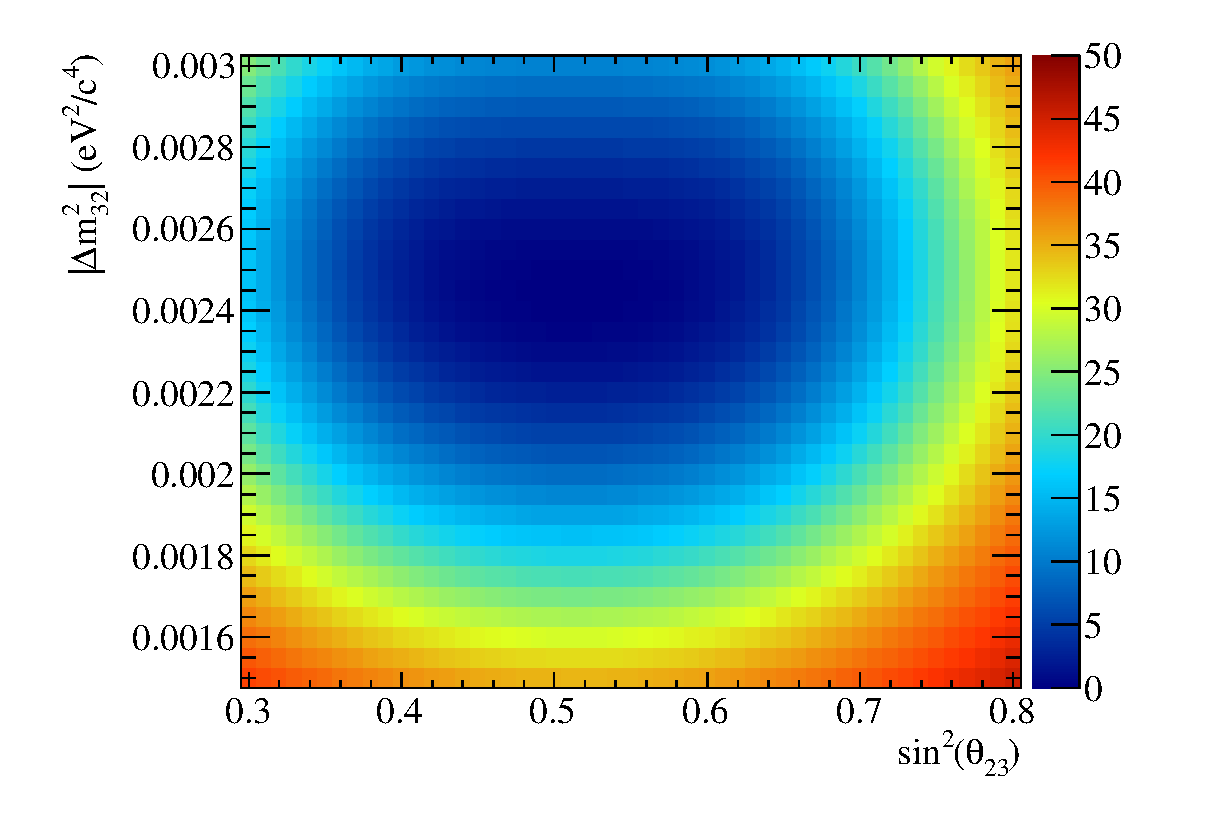
\includegraphics[width=21pc]{./images/fit_data/2Nsintheta/dchisq_3}
\caption {
  $\Delta\chi^2$ surface for the `2+N' $\sin^2\theta_{23}$ fit to the Run 1+2+3 dataset.
}
\label{fig:results_data123_chisq_2Nsintheta}
\end{figure*}

\begin{figure*}[htb]
\begin{minipage}[t]{0.48\linewidth}
\center
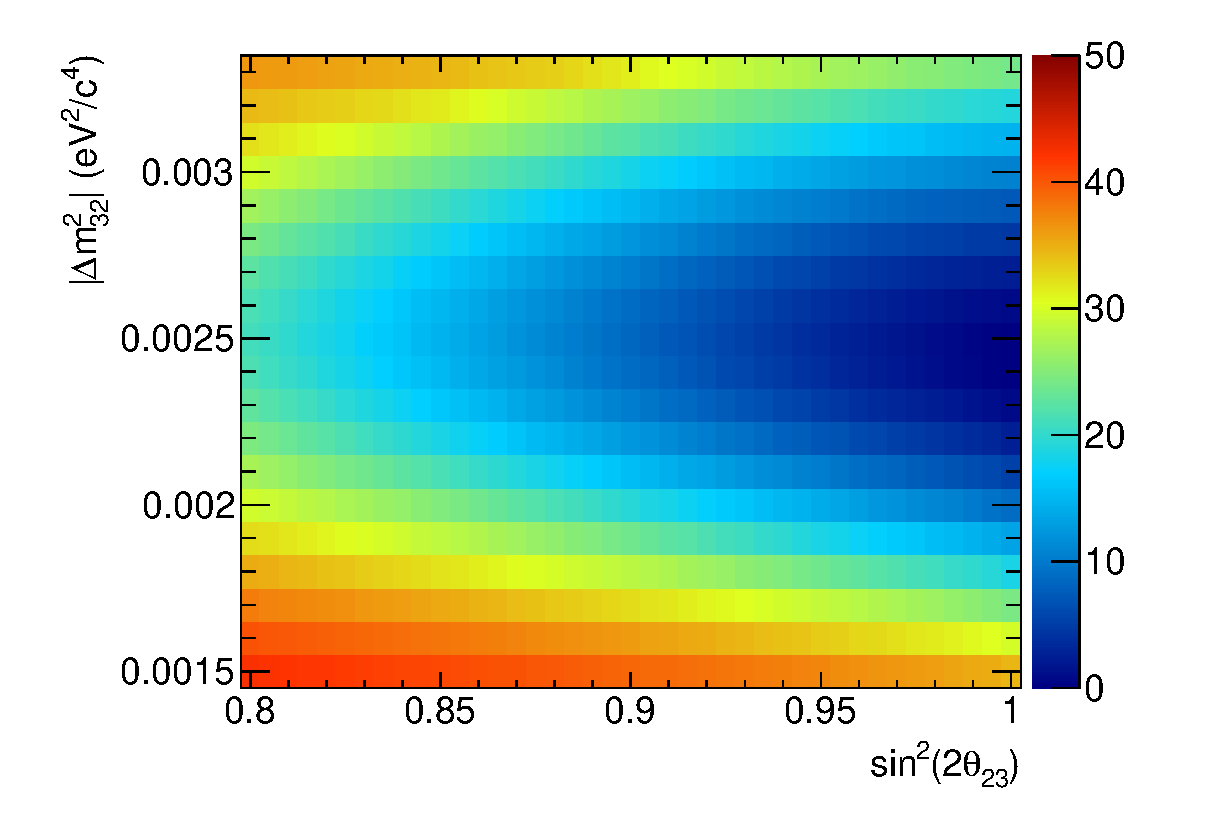
\includegraphics[width=21pc]{./images/fit_data/2N/dchisq_3}
\caption {
  $\Delta\chi^2$ surface for the `2+N' fit to the Run 1+2+3 dataset, assuming $\theta_{23}$ is in the first octant.
}
\label{fig:results_data123_chisq_2N}
\end{minipage}
\hspace{0.06\linewidth}
\begin{minipage}[t]{0.48\linewidth}
\center
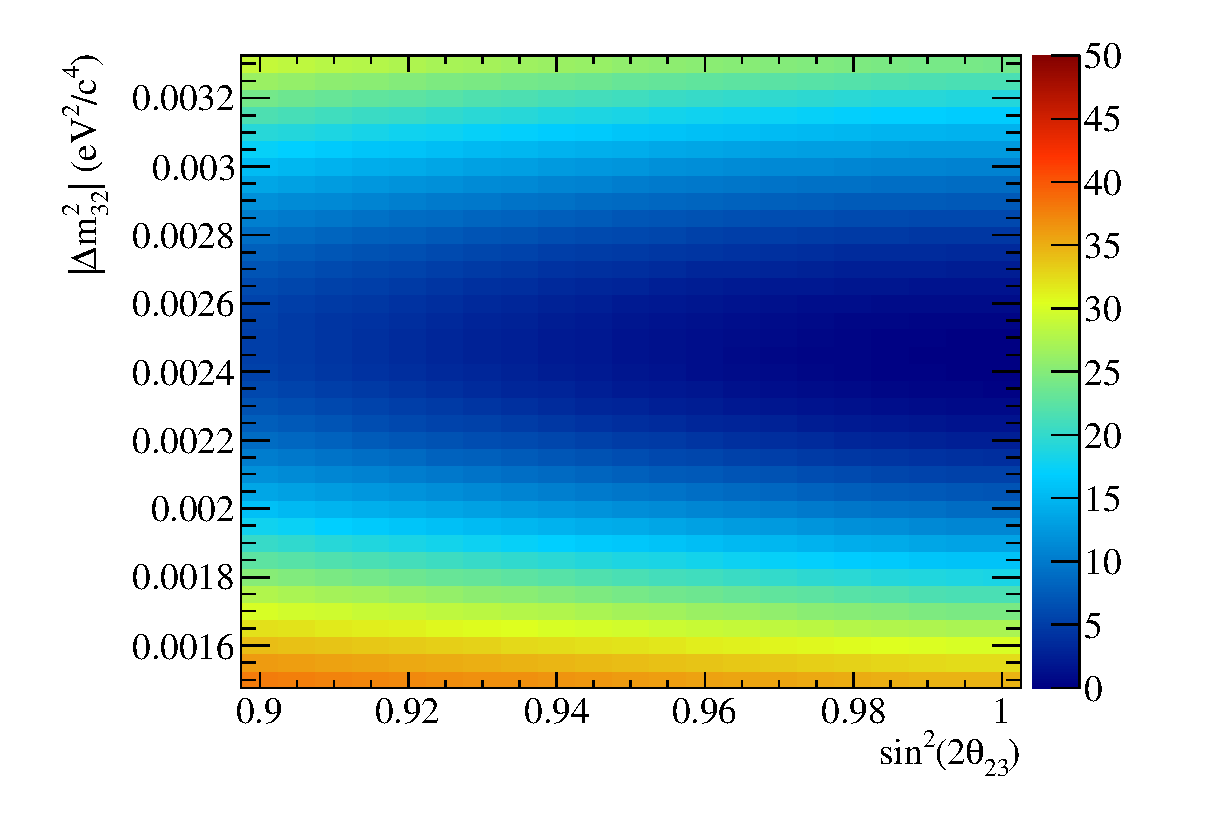
\includegraphics[width=21pc]{./images/fit_data/2Noctant2/dchisq_3}
\caption {
  $\Delta\chi^2$ surface for the `2+N' fit to the Run 1+2+3 dataset, assuming $\theta_{23}$ is in the second octant.
}
\label{fig:results_data123_chisq_2NO2}
\end{minipage}
\end{figure*}

\begin{figure*}[htb]
\begin{minipage}[t]{0.48\linewidth}
\center
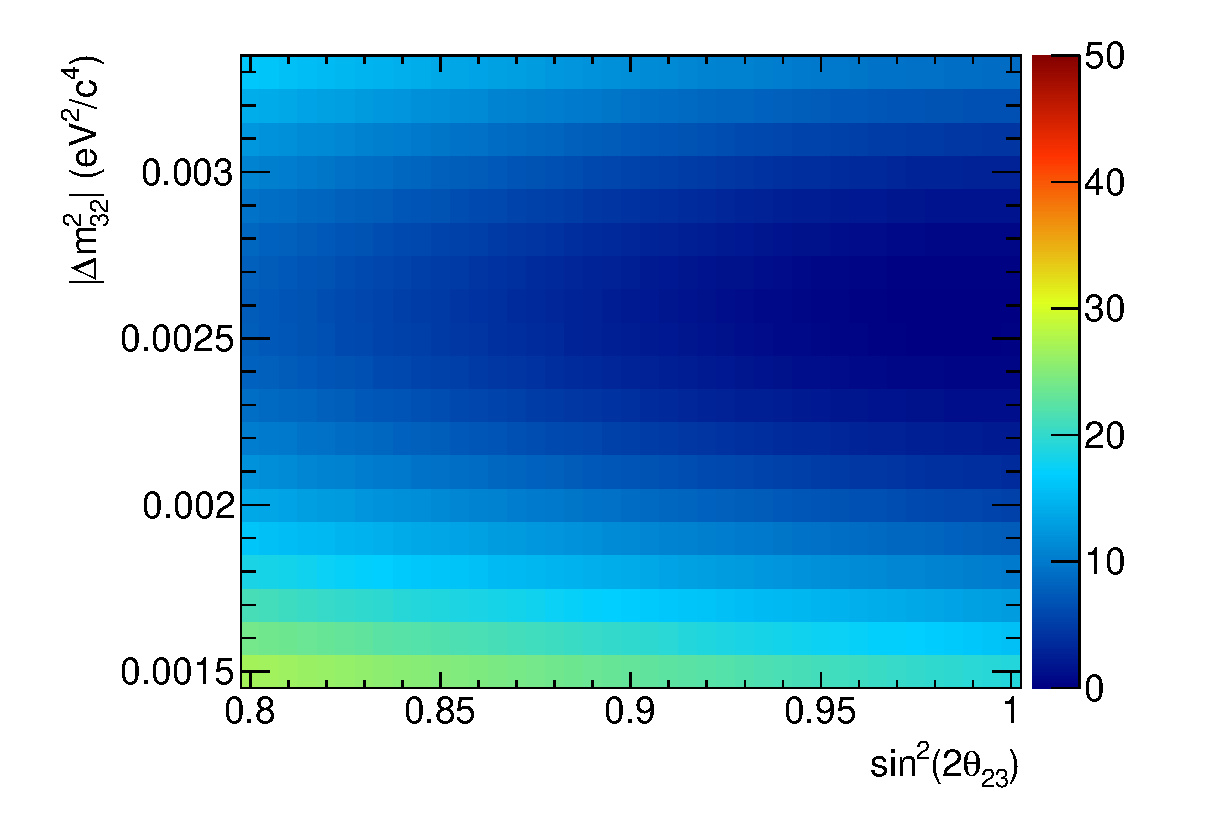
\includegraphics[width=21pc]{./images/fit_data/2N/dchisq_4}
\caption {
  $\Delta\chi^2$ surface for the `2+N' fit to the Run 1+2 dataset.
}
\label{fig:results_data12_chisq_2N}
\end{minipage}
\hspace{0.06\linewidth}
\begin{minipage}[t]{0.48\linewidth}
\center
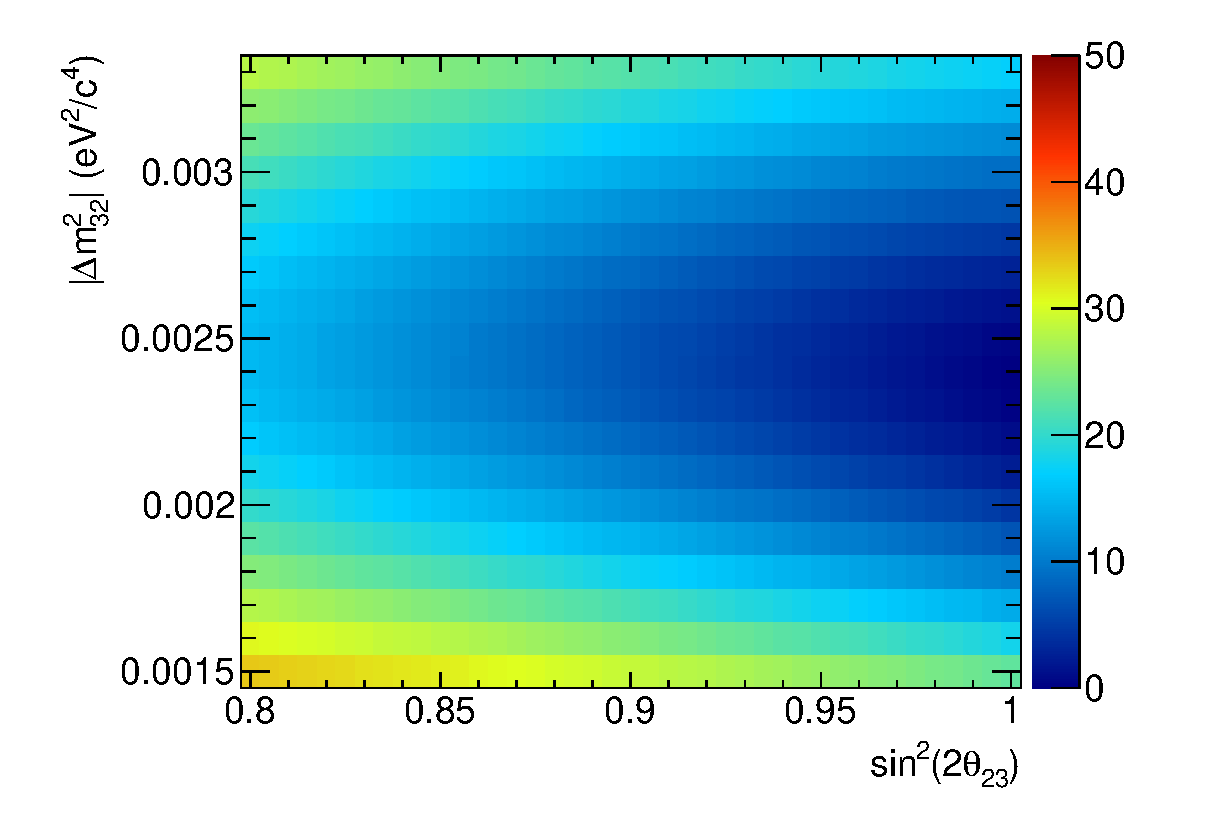
\includegraphics[width=21pc]{./images/fit_data/2N/dchisq_5}
\caption {
  $\Delta\chi^2$ surface for the `2+N' fit to the Run 3 dataset.
}
\label{fig:results_data3_chisq_2N}
\end{minipage}
\end{figure*}

%...........................................................
%
% Marginalised \Delta\chisquare plots for `2+N' fits
%
\begin{figure*}[htb]
\center
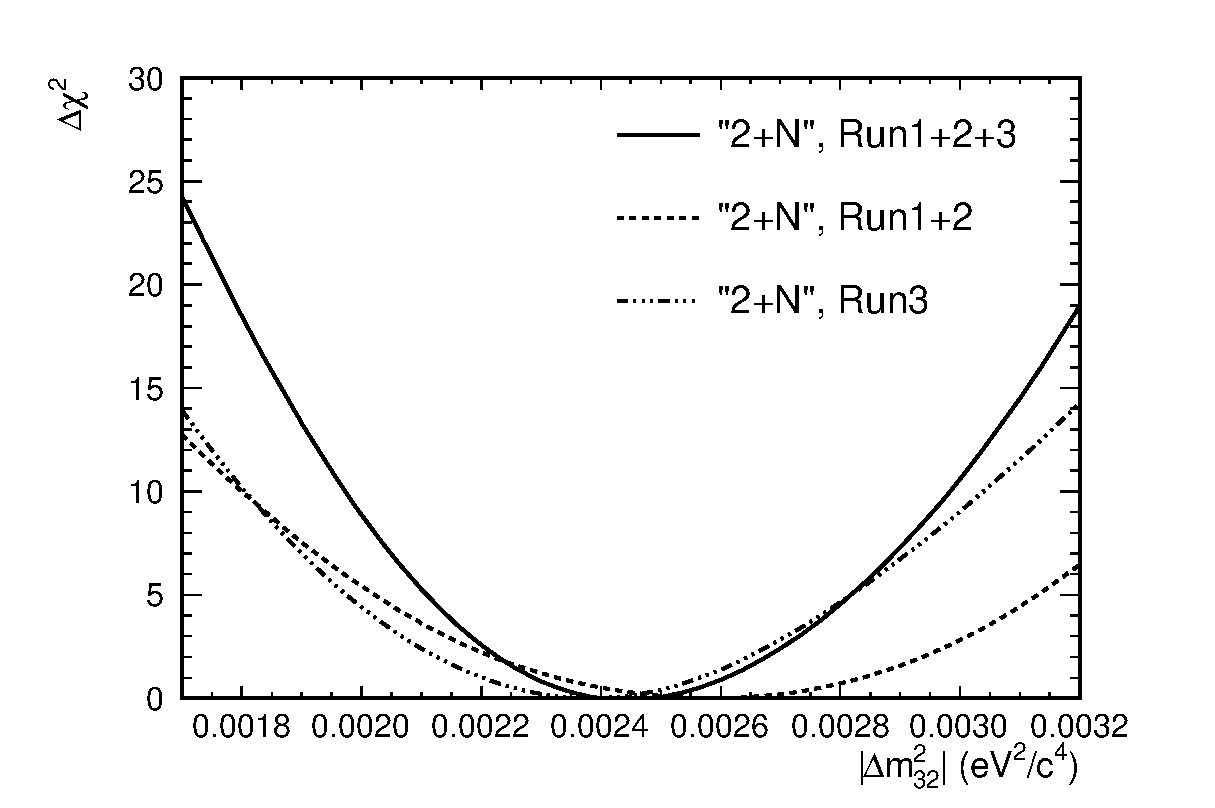
\includegraphics[width=35pc]{./images/fit_data/2N/marg_dchisq_withsyst_dm32sq_2N.eps}
\caption {
  Marginalized $\Delta\chi^2$, as a function of $|\Delta m^{2}_{32}|$, 
  for the four `2+N' fits to the Run 1+2+3, Run 1+2 and Run 3 datasets.
}
\label{fig:results_marg_dchisq_dmsq_all3_2N}
\end{figure*}

\begin{figure*}[htb]
\center
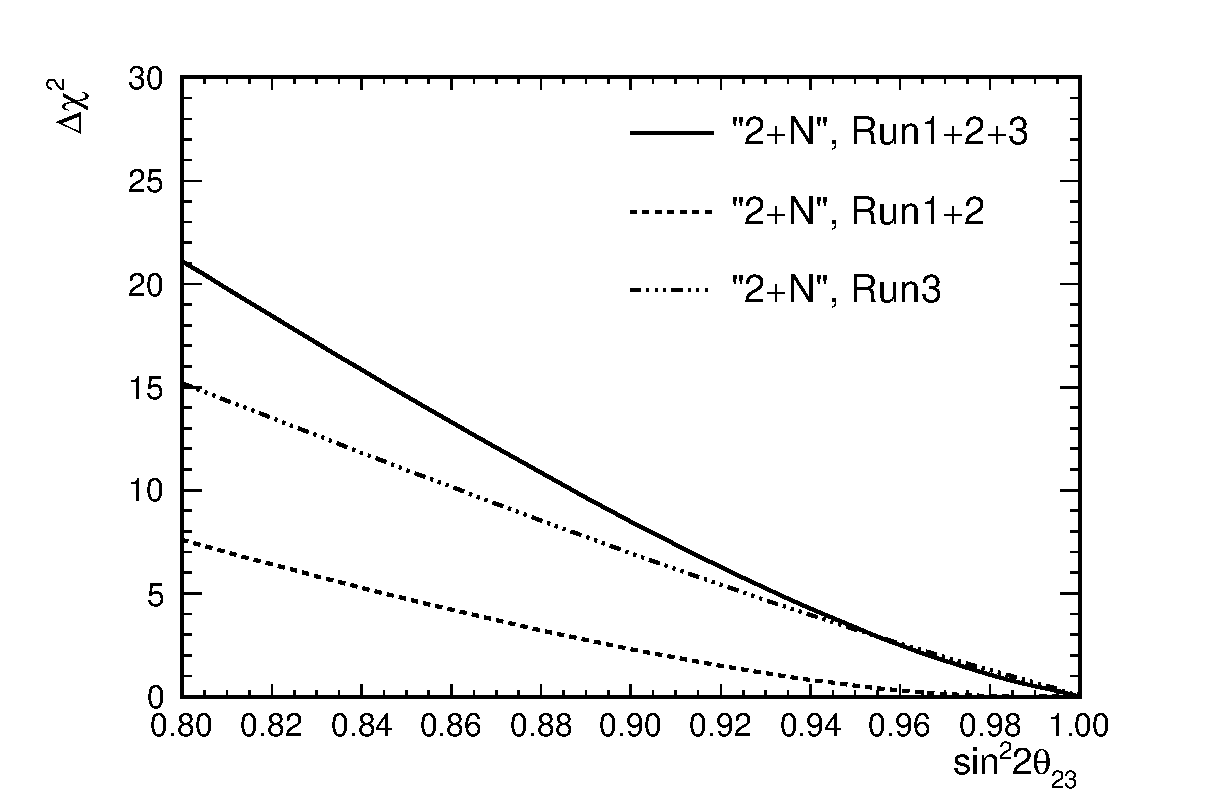
\includegraphics[width=35pc]{./images/fit_data/2N/marg_dchisq_withsyst_sinsq23_2N.eps}
\caption {
  Marginalized $\Delta\chi^2$, as a function of $\sin^{2}2\theta_{23}$, 
  for the three `2+N' fits to the Run 1+2+3, Run 1+2 and Run 3 datasets.
}
\label{fig:results_marg_dchisq_sinsq_all3_2N}
\end{figure*}


%...........................................................
%
% \Delta\chisquare surfaces for `2+8' fits
%
\begin{figure*}[htb]
\center
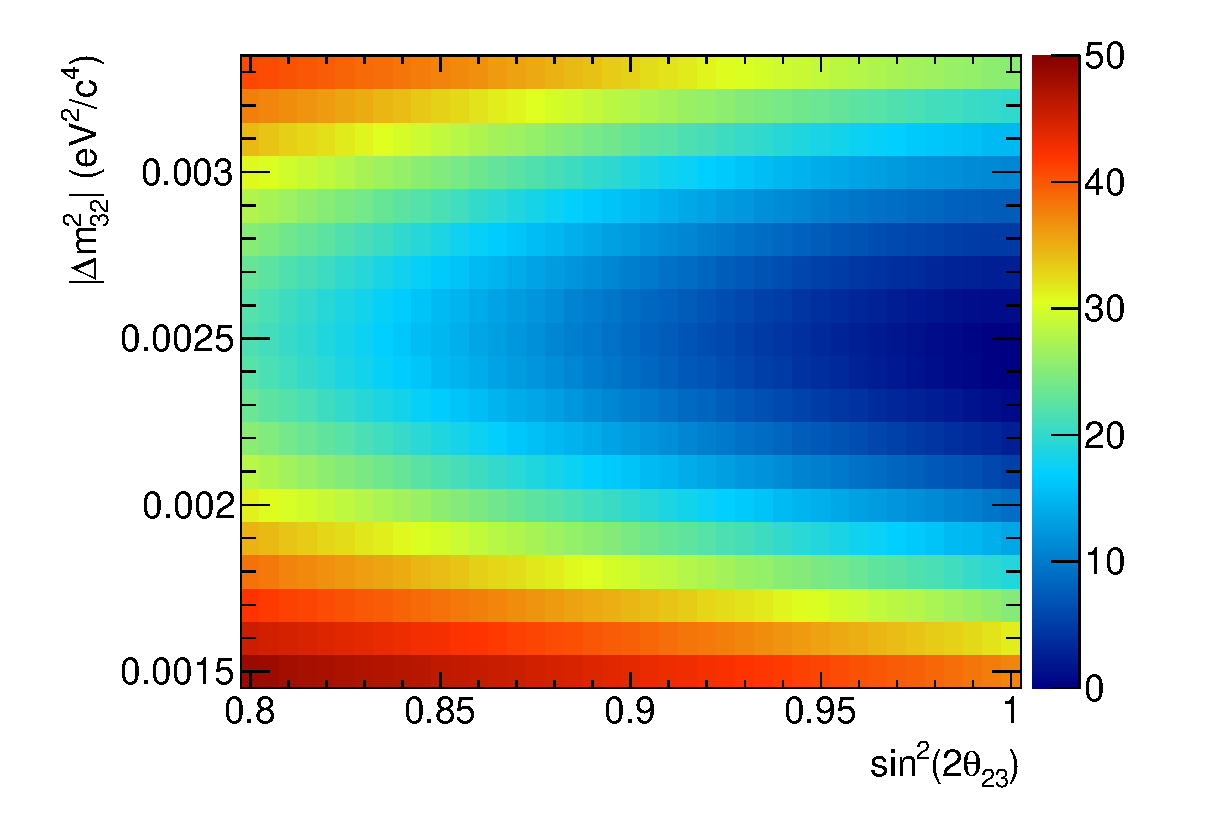
\includegraphics[width=36pc]{./images/fit_data/28/dchisq_3}
\caption {
  $\Delta\chi^2$ surface for the `2+8' fit to the Run 1+2+3 dataset.
}
\label{fig:results_data123_chisq}
\end{figure*}

\begin{figure*}[htb]
\begin{minipage}[t]{0.48\linewidth}
\center
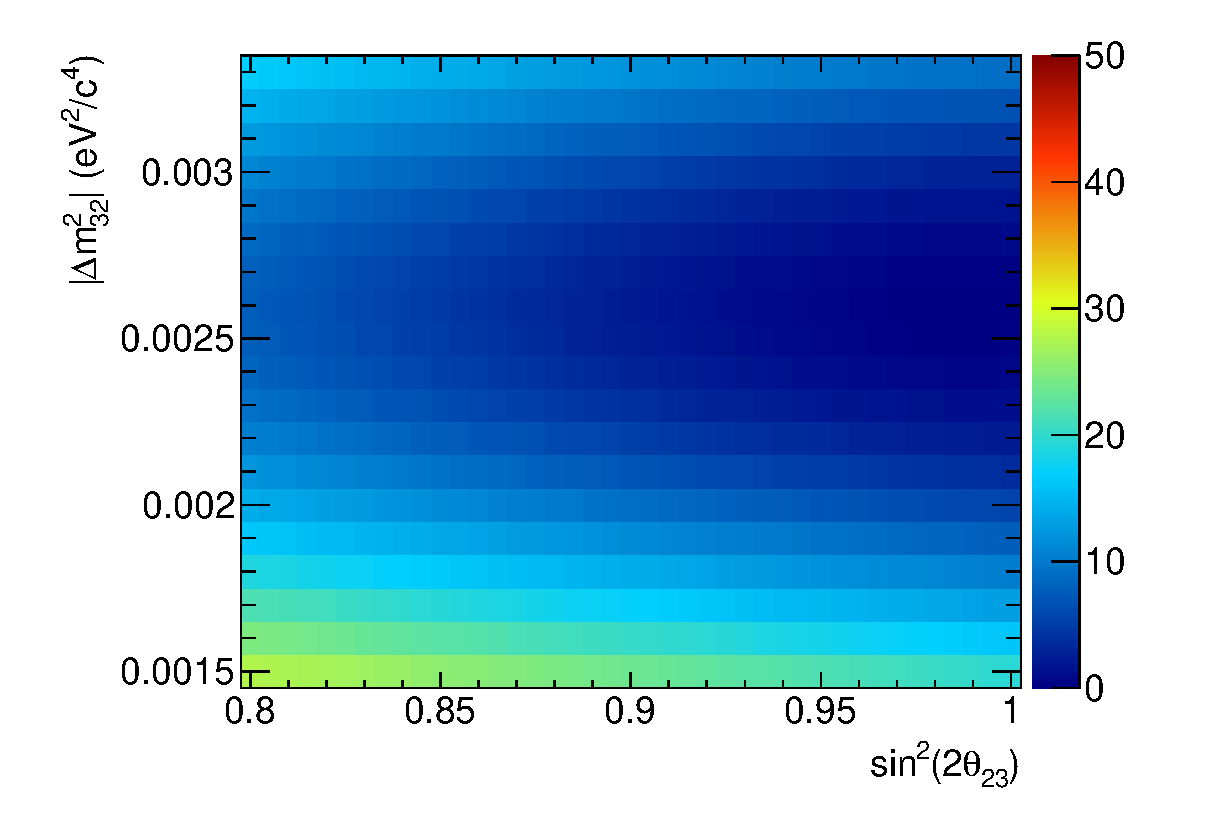
\includegraphics[width=21pc]{./images/fit_data/28/dchisq_4}
\caption {
  $\Delta\chi^2$ surface for the `2+8' fit to the Run 1+2 dataset.
}
\label{fig:results_data12_chisq}
\end{minipage}
\hspace{0.06\linewidth}
\begin{minipage}[t]{0.48\linewidth}
\center
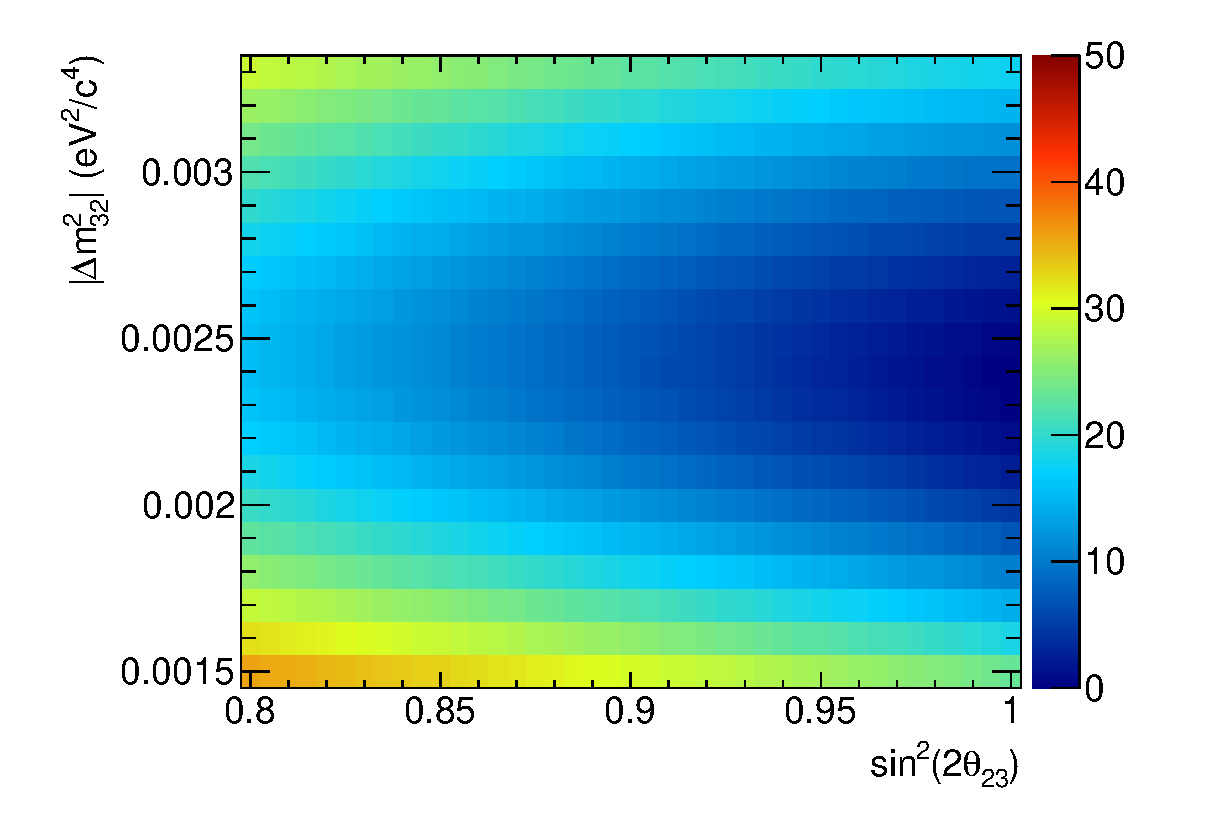
\includegraphics[width=21pc]{./images/fit_data/28/dchisq_5}
\caption {
  $\Delta\chi^2$ surface for the `2+8' fit to the Run 3 dataset.
}
\label{fig:results_data3_chisq}
\end{minipage}
\end{figure*}

%...........................................................
%
% Marginalised \Delta\chisquare plots for `2+8' fits
%
\begin{figure*}[htb]
\center
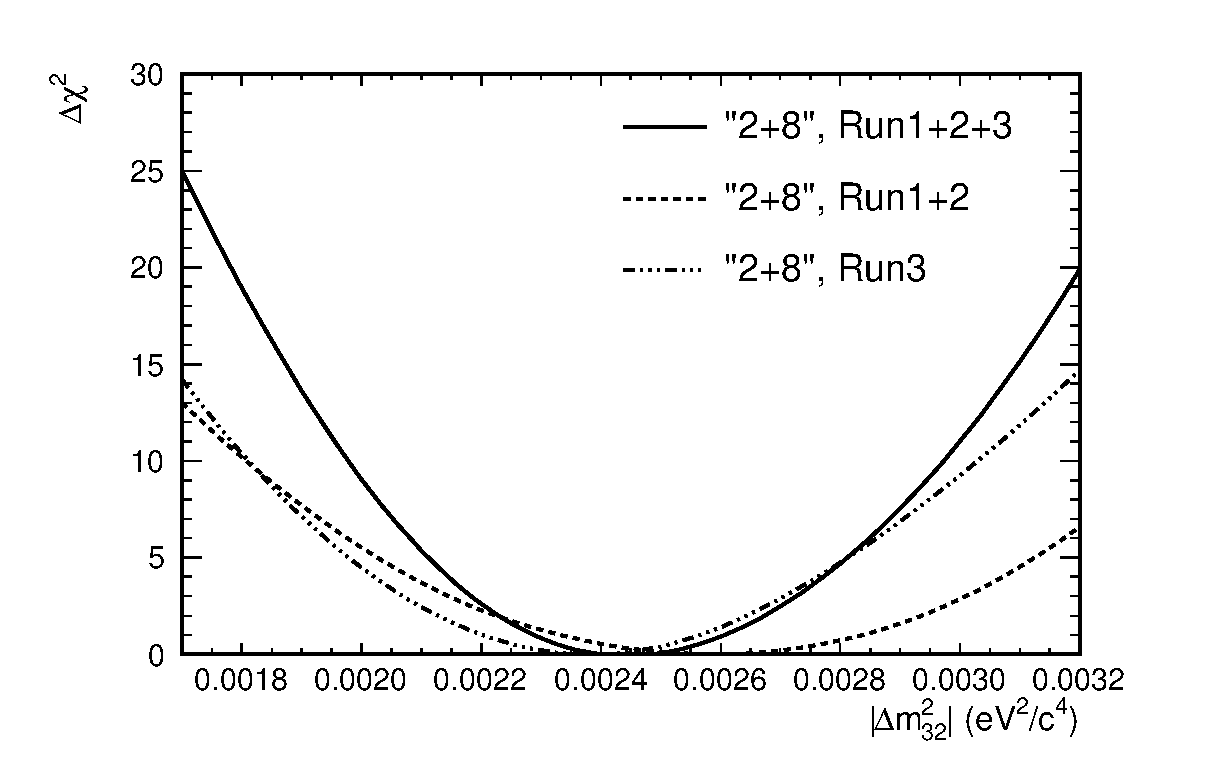
\includegraphics[width=35pc]{./images/fit_data/28/marg_dchisq_withsyst_dm32sq_28.eps}
\caption {
  Marginalized $\Delta\chi^2$, as a function of $|\Delta m^{2}_{32}|$, 
  for the three `2+8' fits to the Run 1+2+3, Run 1+2 and Run 3 datasets.
}
\label{fig:results_marg_dchisq_dmsq_all3}
\end{figure*}

\begin{figure*}[htb]
\center
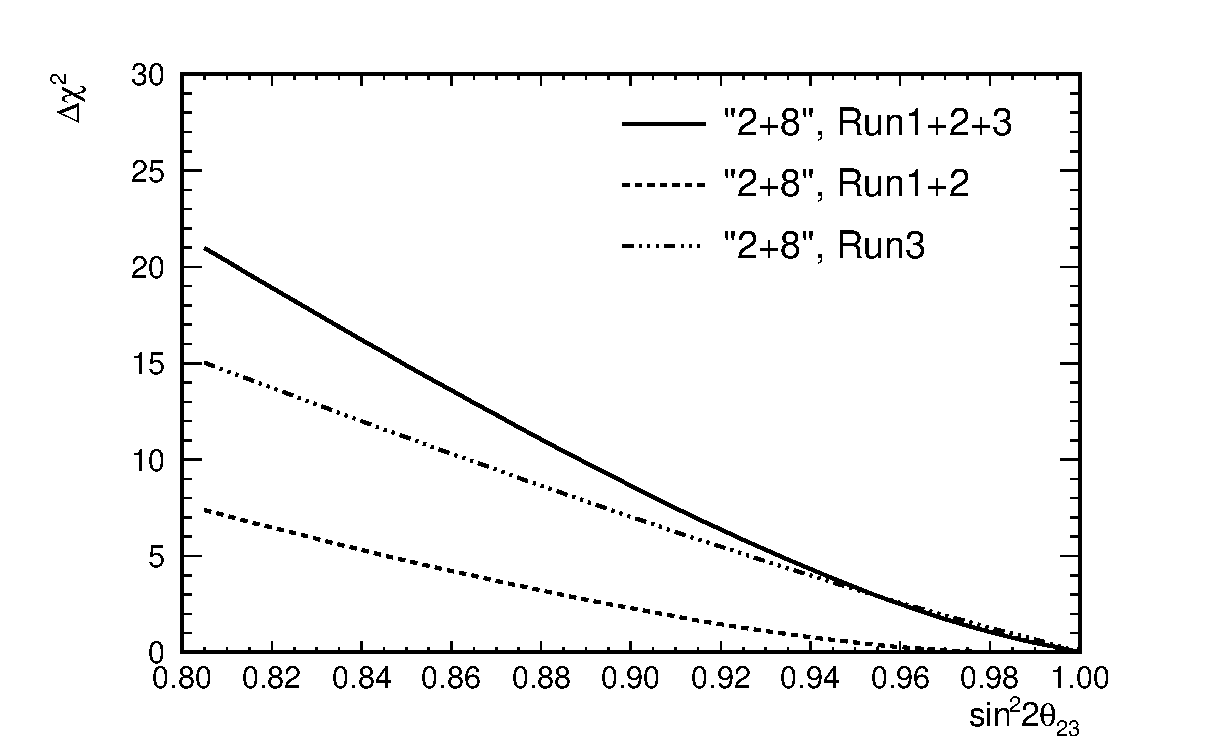
\includegraphics[width=35pc]{./images/fit_data/28/marg_dchisq_withsyst_sinsq23_28.eps}
\caption {
  Marginalized $\Delta\chi^2$, as a function of $\sin^{2}2\theta_{23}$, 
  for the three `2+8' fits to the Run 1+2+3, Run 1+2 and Run 3 datasets.
}
\label{fig:results_marg_dchisq_sinsq_all3}
\end{figure*}

%...........................................................
%
% Comparison of `2+N' first and second octant
% \Delta\chisquare surfaces and
% marginalised \Delta\chisquare distributions
%

\begin{figure*}[htb]
%\begin{minipage}[t]{0.48\linewidth}
\center
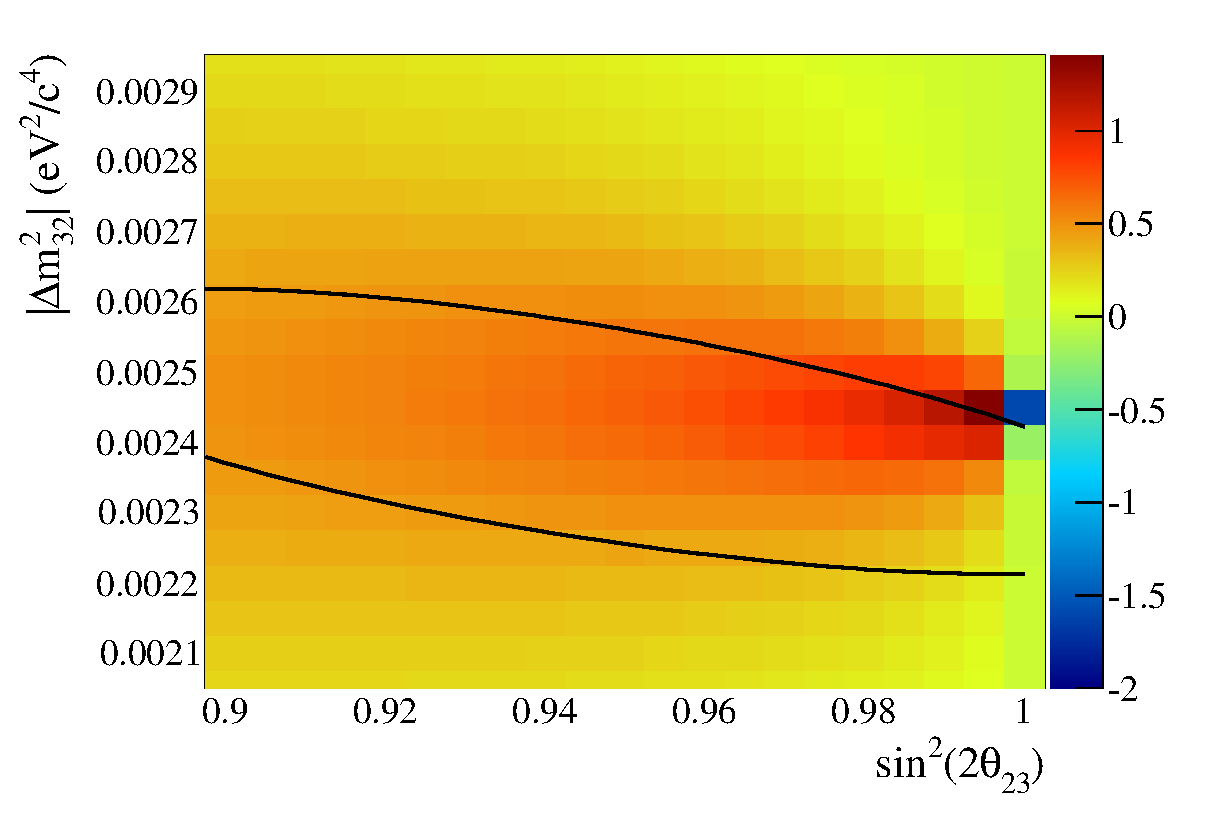
\includegraphics[width=20pc]{./images/fit_data/compare/compare_octants_dchisqdiff_nM8OnP8O2}
\caption {
  Fractional difference between the $\Delta\chi^2$ surfaces
  obtained from the `2+N' fits to the Run 1+2+3 dataset assuming $\theta_{23}$ is in the first and second octants
  and shown in Figs.\ \ref{fig:results_data123_chisq_2N} and \ref{fig:results_data123_chisq_2NO2}.
  The fractional difference is calculated as 
  2 $\times$ ($\Delta\chi^2$(octant 1)-$\Delta\chi^2$(octant 2)) / $\Delta\chi^2$(octant 1)+$\Delta\chi^2$(octant 2)).
  The 2012 MINOS 90\% CL region is shown for reference.
  The large difference at the minimum of the $\Delta \chi^2$ maps is due to the best fit point in the
  second octant case being further away from a bin center.
}
\label{fig:results_dchisq_fracdiff_run123_octant}
%\end{minipage}
% \hspace{0.06\linewidth}
% \begin{minipage}[t]{0.48\linewidth}
% \center
% % \includegraphics[width=20pc]{./images/fit_data/compare/compare_octants_dchisqdiff_nM8OnP8O2_zoom}
% 
\includegraphics[width=20pc]{./images/placeholder}
% \caption {
%   As on the left but zoomed into the area of the 2012 MINOS 90\% CL region.
% }
% \label{fig:results_dchisq_fracdiff_run123_octant_zoom}
% \end{minipage}
\end{figure*}

%---

% \begin{figure*}[htb]
% \begin{minipage}[t]{0.48\linewidth}
% \center
% 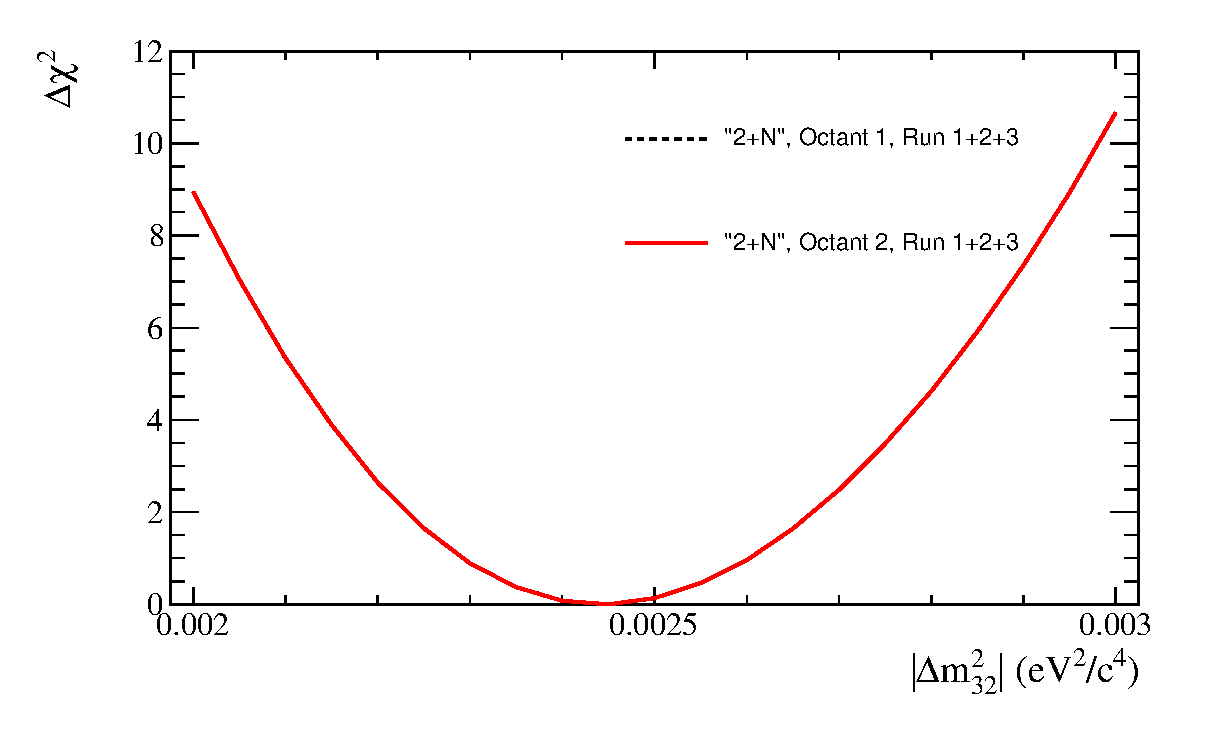
\includegraphics[width=20pc]{./images/fit_data/compare/marg_dchisq_withsyst_dm23sq_2N_2NO2_comp.eps}
% \caption {
%   Comparison of marginalized $\Delta\chi^2$ as a function of $|\Delta m^{2}_{32}|$, 
%   for the `2+N' fits to the Run 1+2+3 dataset, for both octant assumptions.
% }
% \label{fig:results_comp_marg_dchisq_dmsq_run123_octant}
% \end{minipage}
% \hspace{0.06\linewidth}
% \begin{minipage}[t]{0.48\linewidth}
% \center
% 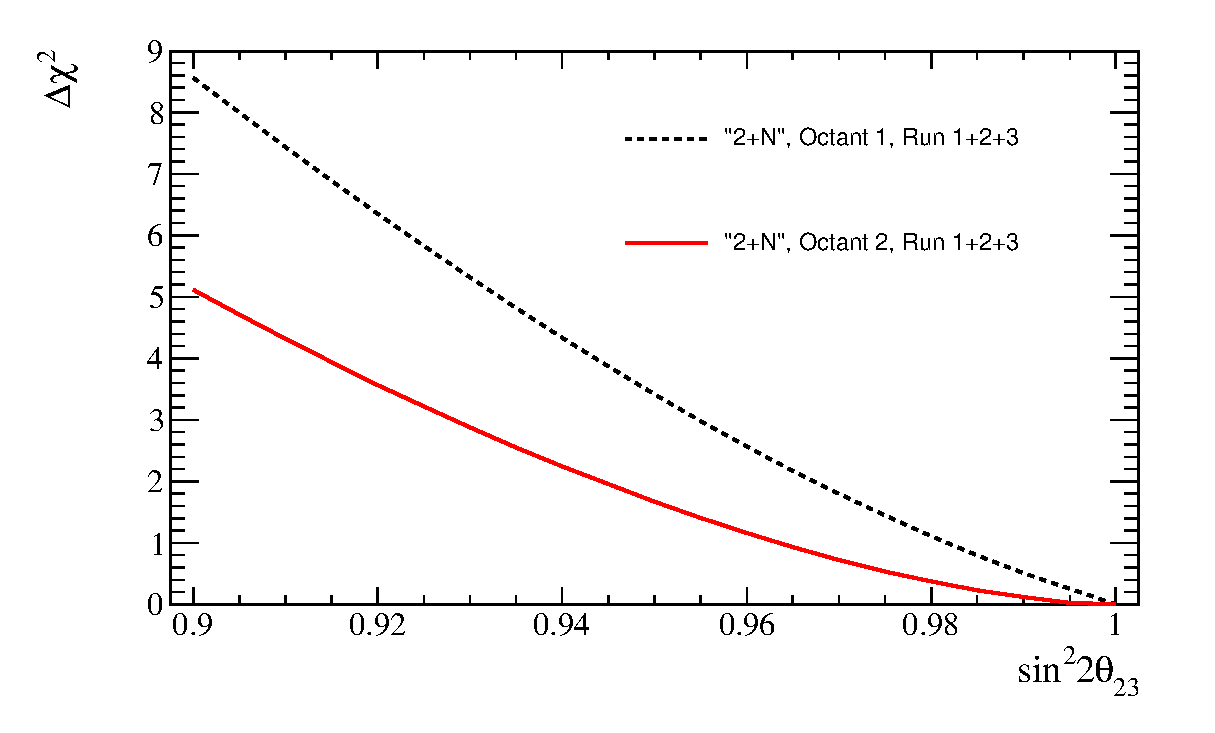
\includegraphics[width=20pc]{./images/fit_data/compare/marg_dchisq_withsyst_sinsq23_2N_2NO2_comp.eps}
% \caption {
%   Comparison of marginalized $\Delta\chi^2$ as a function of $\sin^{2}2\theta_{23}$, 
%   for the `2+N' fits to the Run 1+2+3 dataset, for both octant assumptions.
% }
% \label{fig:results_comp_marg_dchisq_sinsq_run123_octant}
% \end{minipage}
% \end{figure*}


%...........................................................
%
% Comparison of `2+N' and `2+8' 
% \Delta\chisquare surfaces and
% marginalised \Delta\chisquare distributions
%

\begin{figure*}[htb]
\begin{minipage}[t]{0.48\linewidth}
\center
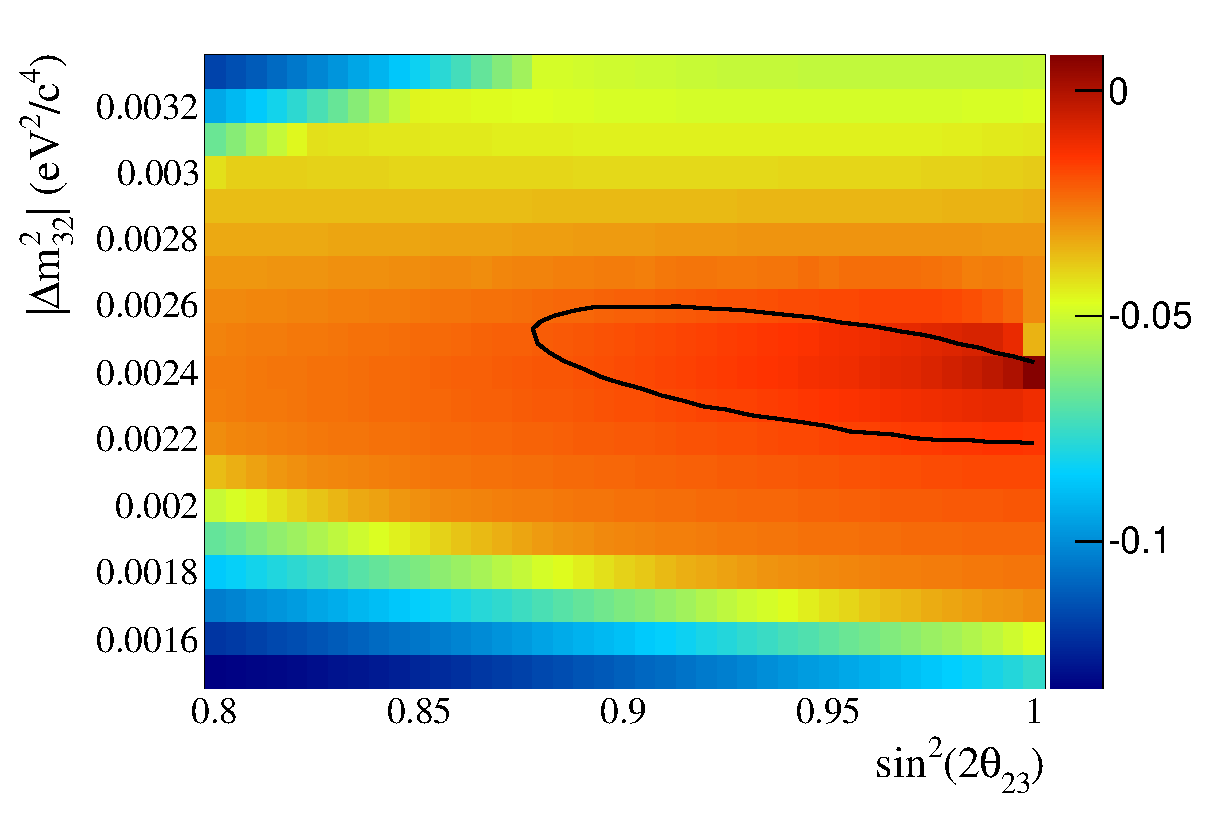
\includegraphics[width=20pc]{./images/fit_data/compare/compare_2all_28_dchisqdiff_nM8OnP8O2}
\caption {
  Fractional difference between the $\Delta\chi^2$ surfaces
  obtained from the `2+N' and `2+8' fits to the Run 1+2+3 dataset 
  and shown in Figs.\ \ref{fig:results_data123_chisq_2N} and \ref{fig:results_data123_chisq}.
  The fractional difference is calculated as 
  2 $\times$ ($\Delta\chi^2$(`2+N')-$\Delta\chi^2$(`2+8')) / $\Delta\chi^2$(`2+N')+$\Delta\chi^2$(`2+8')).
  The 2012 MINOS 90\% CL region is shown for reference.
}
\label{fig:results_dchisq_fracdiff_run123}
\end{minipage}
\hspace{0.06\linewidth}
\begin{minipage}[t]{0.48\linewidth}
\center
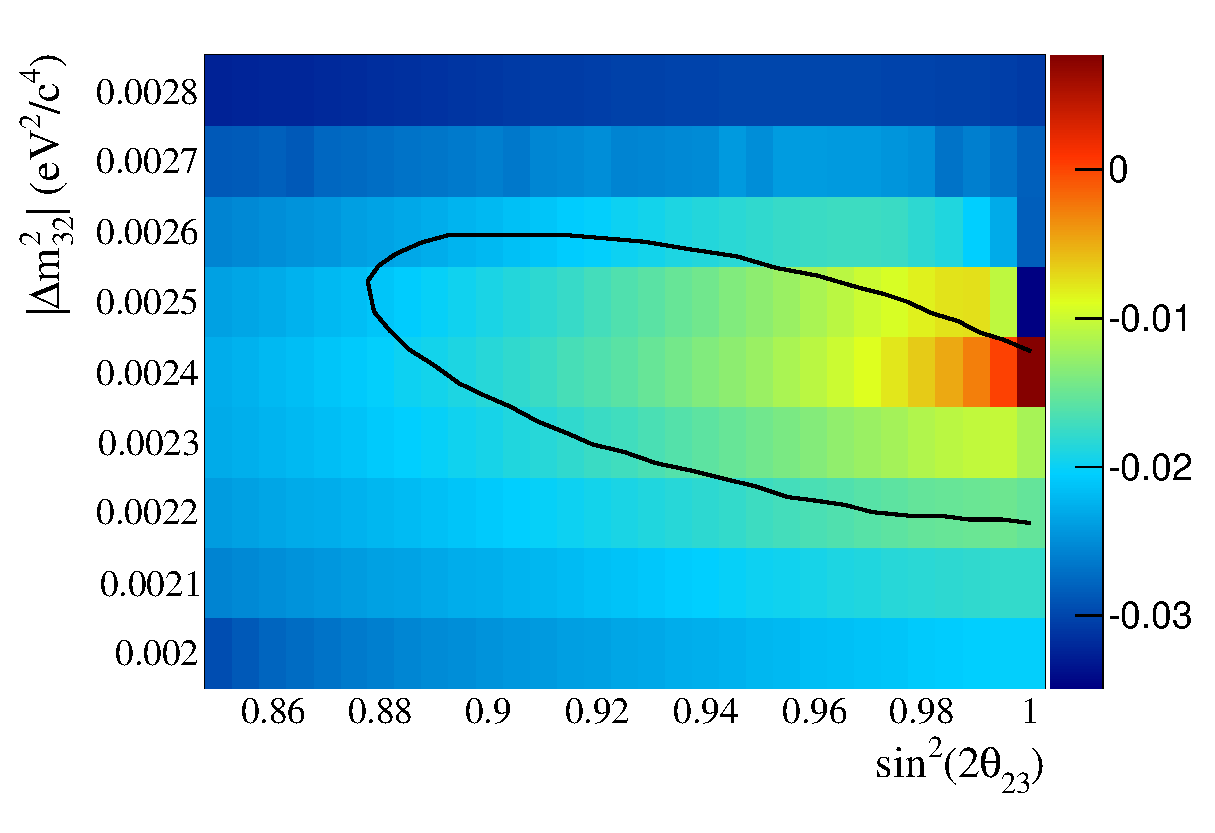
\includegraphics[width=20pc]{./images/fit_data/compare/compare_2all_28_dchisqdiff_nM8OnP8O2_zoom} 
\caption {
  As on the left but zoomed into the area of the 2012 MINOS 90\% CL region.
}
\label{fig:results_dchisq_fracdiff_run123_zoom}
\end{minipage}
\end{figure*}

%---

\begin{figure*}[htb]
\begin{minipage}[t]{0.48\linewidth}
\center
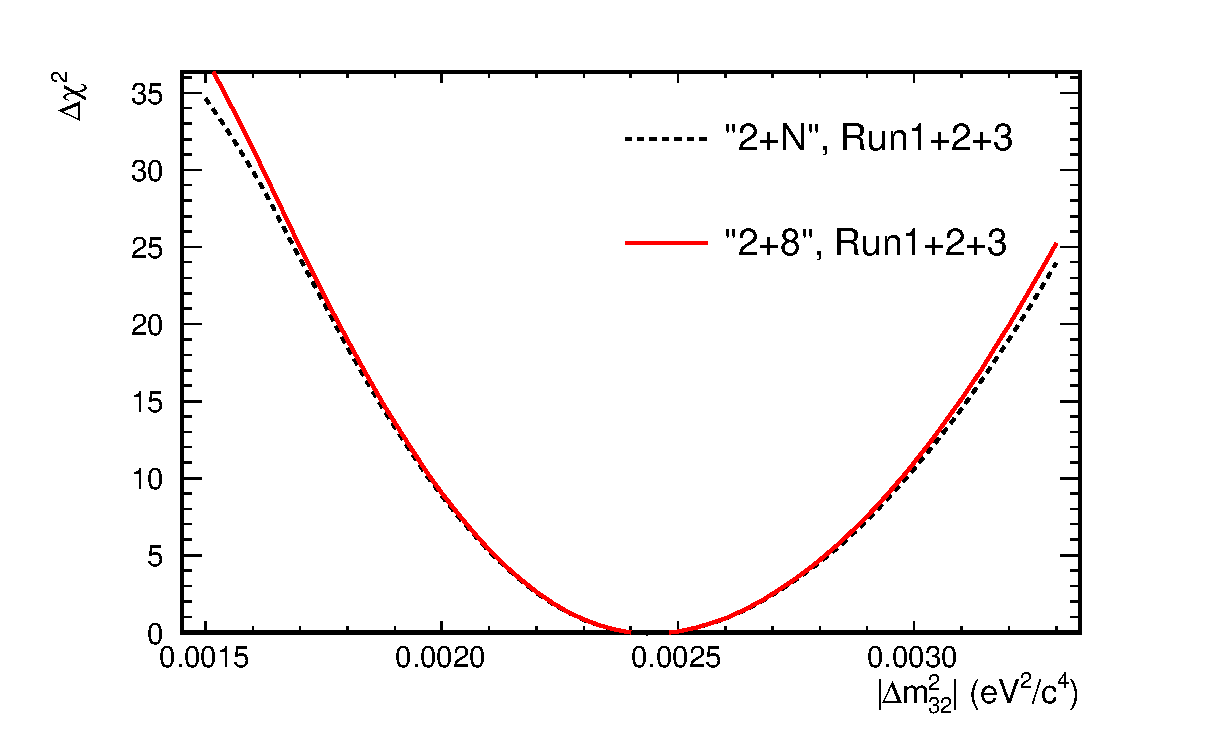
\includegraphics[width=20pc]{./images/fit_data/compare/marg_dchisq_withsyst_dm23sq_2N_28_comp.eps}
\caption {
  Comparison of marginalized $\Delta\chi^2$ as s function of $|\Delta m^{2}_{32}|$, 
  for the `2+N' and `2+8' fits to the Run 1+2+3 dataset.
}
\label{fig:results_comp_marg_dchisq_dmsq_run123}
\end{minipage}
\hspace{0.06\linewidth}
\begin{minipage}[t]{0.48\linewidth}
\center
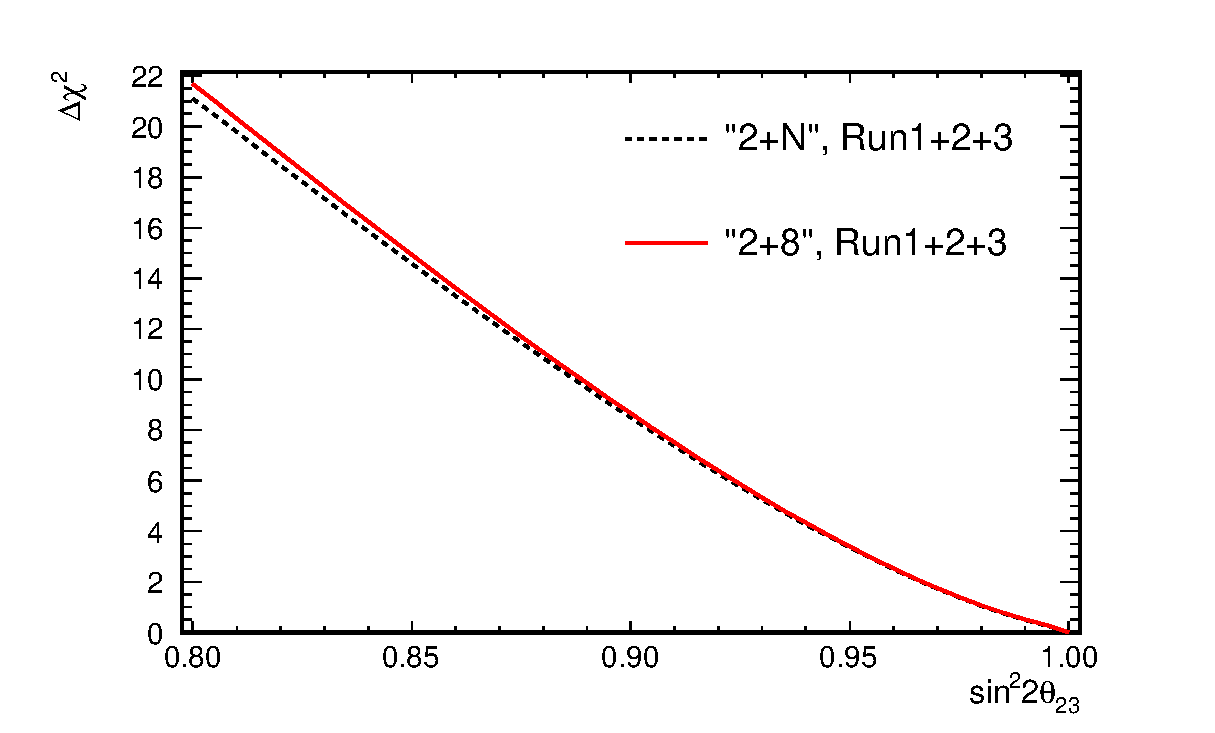
\includegraphics[width=20pc]{./images/fit_data/compare/marg_dchisq_withsyst_sinsq23_2N_28_comp.eps}
\caption {
  Comparison of marginalized $\Delta\chi^2$ as a function of $\sin^{2}2\theta_{23}$, 
  for the `2+N' and `2+8' fits to the Run 1+2+3 dataset.
}
\label{fig:results_comp_marg_dchisq_sinsq_run123}
\end{minipage}
\end{figure*}

%...........................................................
%
% Const-dchi^2  contours for `2+N' fits
%

\clearpage

\begin{figure*}[htb]
\center
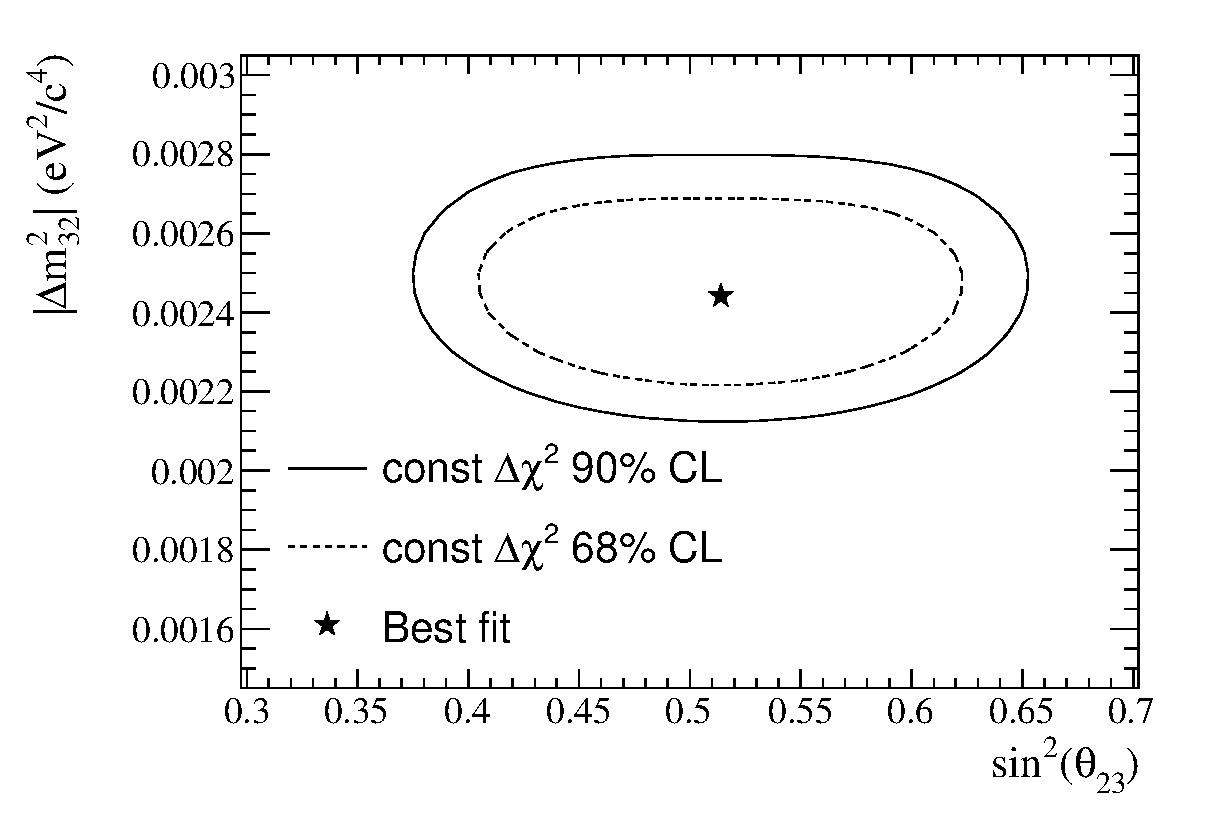
\includegraphics[width=30pc]{./images/fit_data/2Nsintheta/contours_3}
\caption {
  68\% CL and 90\% CL allowed region (including systematics), 
  constructed with the constant-$\Delta\chi^{2}$ method,
  for the `2+N' $\sin^2\theta_{23}$ fit to the Run 1+2+3 dataset.
  The `2+N' best-fit point is also shown.
}
\label{fig:results_data123_contour_2Nsintheta}
\end{figure*}


\begin{figure*}[htb]
\center
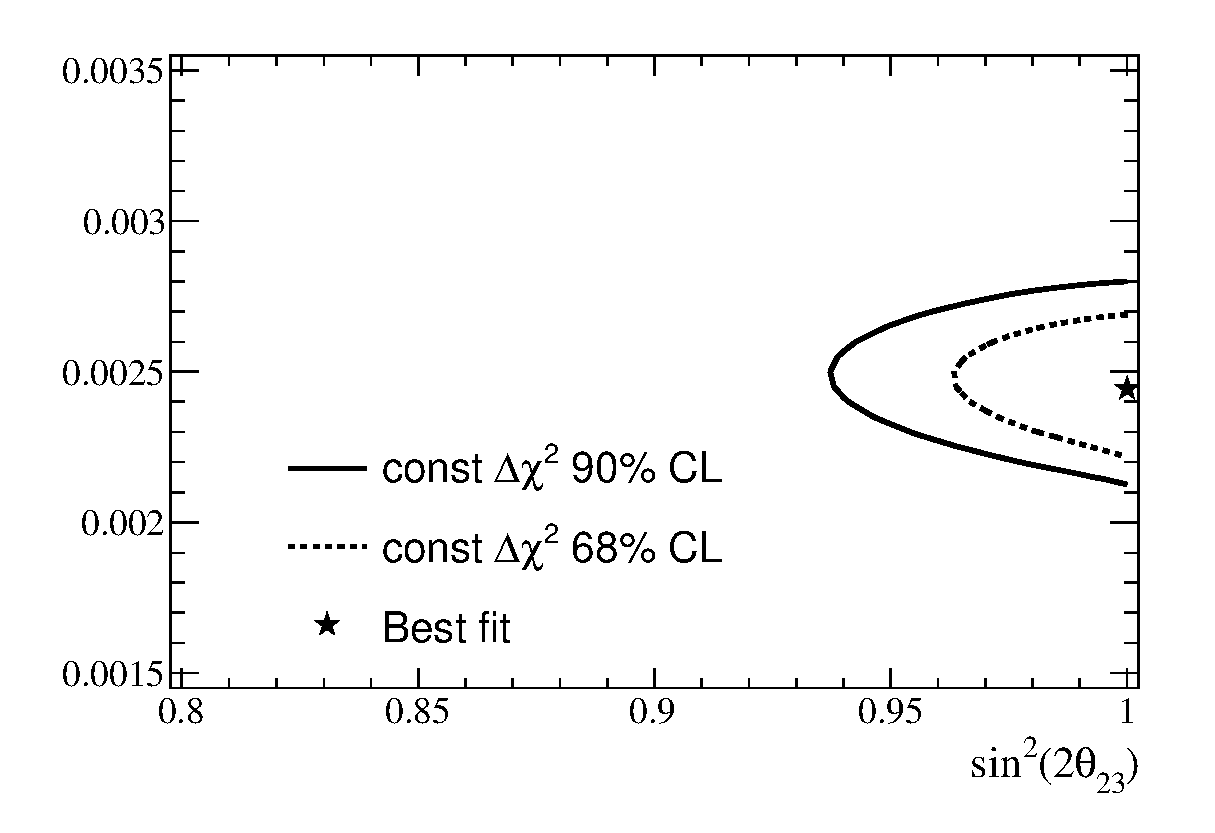
\includegraphics[width=30pc]{./images/fit_data/2N/contours_3}
\caption {
  68\% CL and 90\% CL allowed region (including systematics), 
  constructed with the constant-$\Delta\chi^{2}$ method,
  for the `2+N' fit to the Run 1+2+3 dataset assuming $\theta_{23}$ is in the first octant.
  The `2+N' best-fit point is also shown.
}
\label{fig:results_data123_contour_2N}
\end{figure*}

\begin{figure*}[htb]
\center
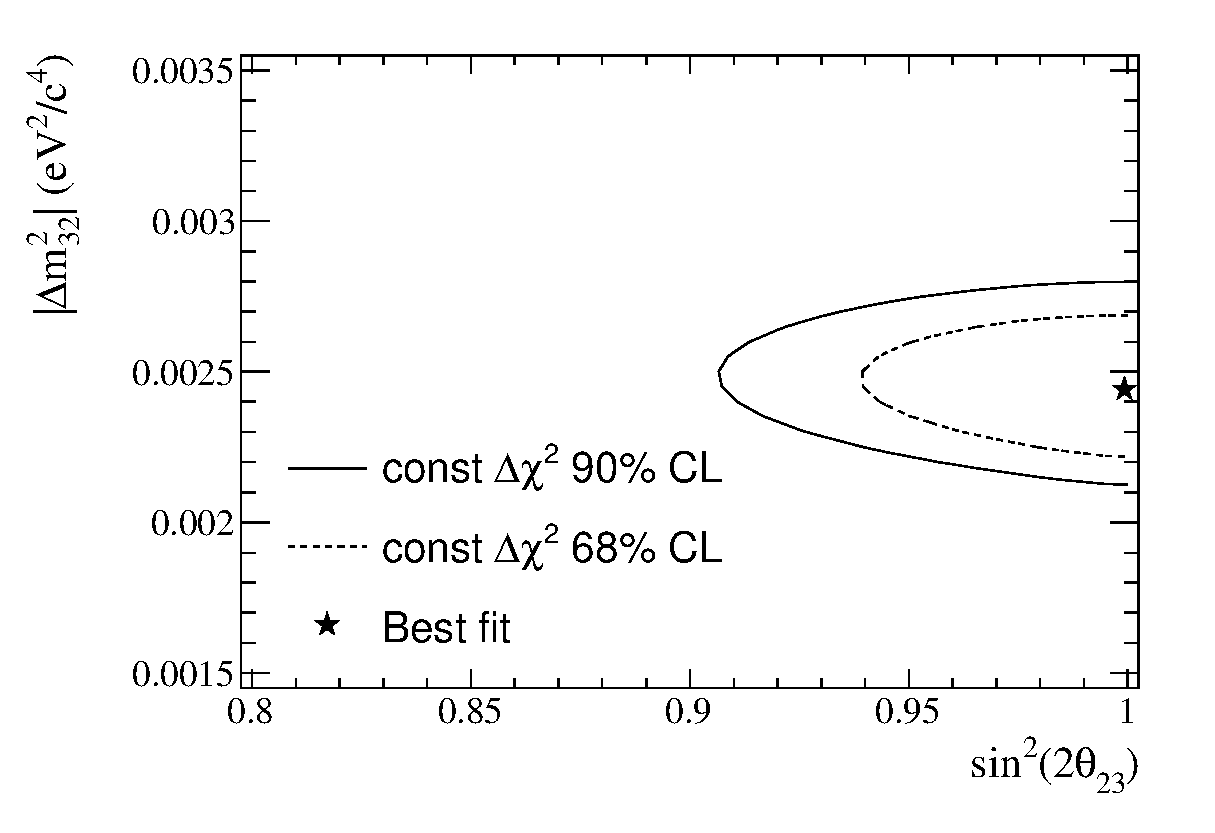
\includegraphics[width=30pc]{./images/fit_data/2Noctant2/contours_3}
\caption {
  68\% CL and 90\% CL allowed region (including systematics), 
  constructed with the constant-$\Delta\chi^{2}$ method,
  for the `2+N' fit to the Run 1+2+3 dataset assuming $\theta_{23}$ is in the second octant.
  The `2+N' best-fit point is also shown.
}
\label{fig:results_data123_contour_2NO2}
\end{figure*}

\begin{figure*}[htb]
\begin{minipage}[t]{0.9\linewidth}
\center
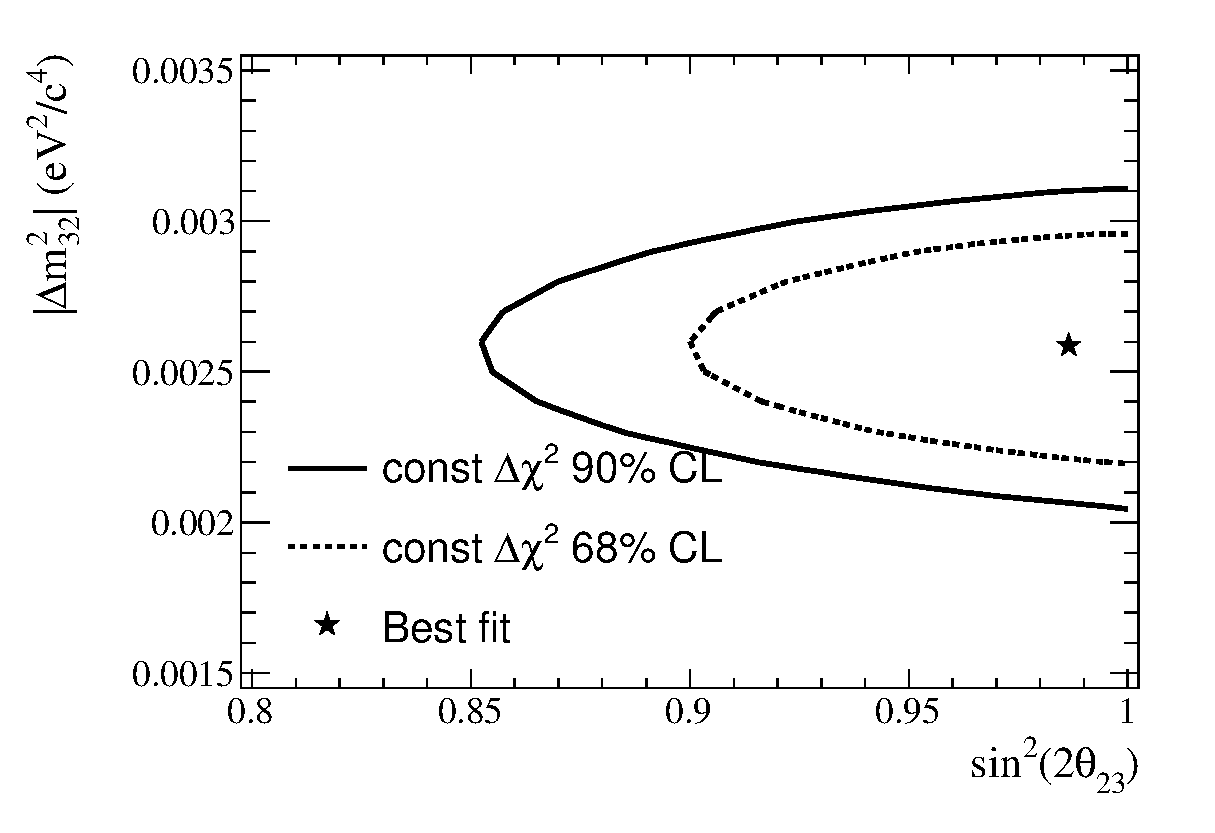
\includegraphics[width=25pc]{./images/fit_data/2N/contours_4}
\caption {
  As in Fig.\ \ref{fig:results_data123_contour_2N}, but for the Run 1+2 dataset only.
}
\label{fig:results_data12_contour_2N}
\end{minipage}
\vfill%\hspace{0.06\linewidth}
\begin{minipage}[t]{0.9\linewidth}
\center
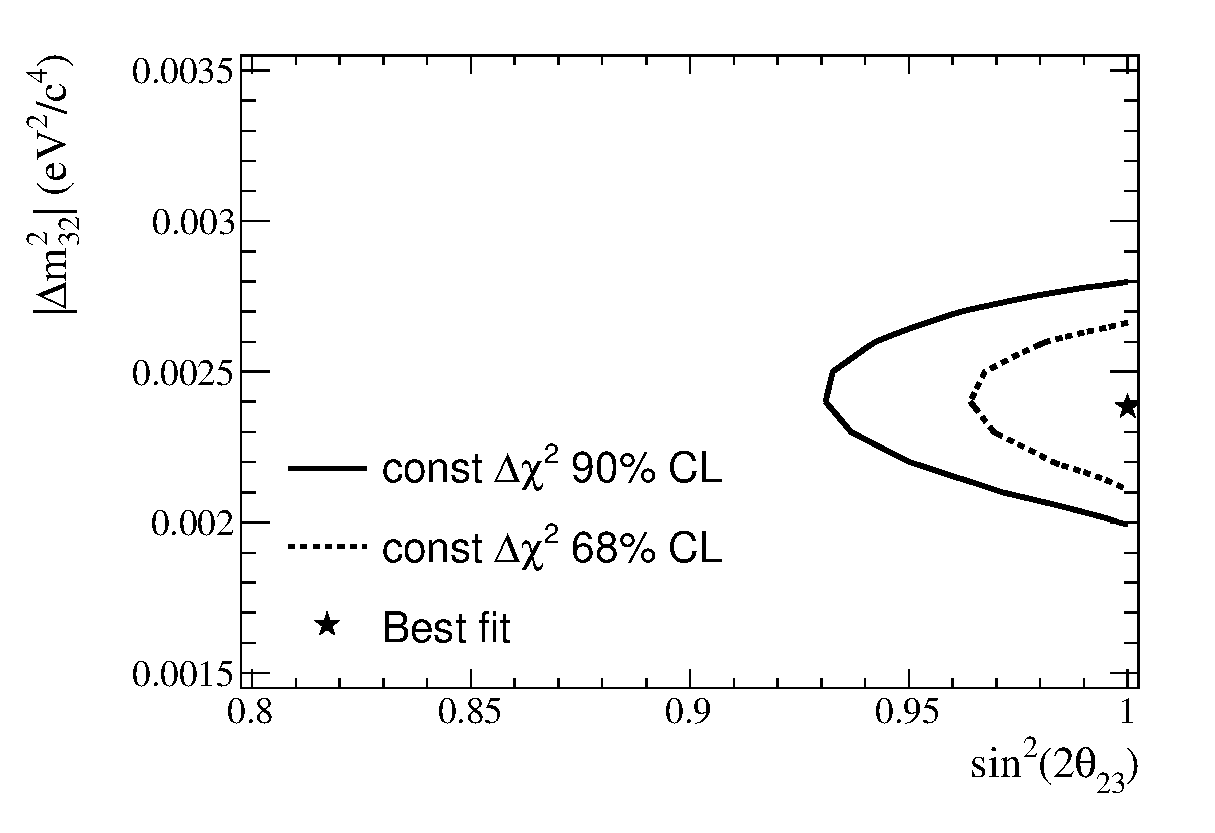
\includegraphics[width=25pc]{./images/fit_data/2N/contours_5}
\caption {
  As in Fig.\ \ref{fig:results_data123_contour_2N}, but for the Run 3 dataset only.
}
\label{fig:results_data3_contour_2N}
\end{minipage}
\end{figure*}


%...........................................................
%
% Const-dchi^2  contours for `2+8' fits
%
\begin{figure*}[htb]
\center
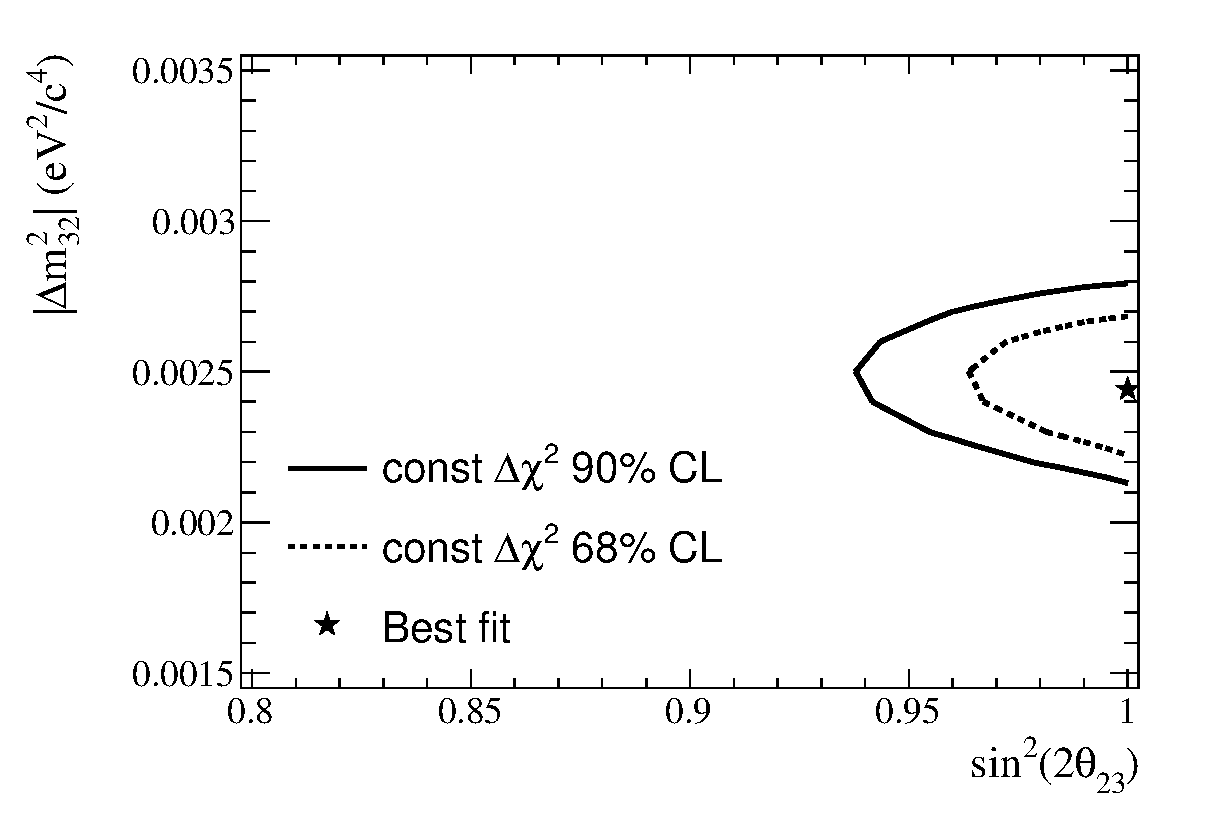
\includegraphics[width=35pc]{./images/fit_data/28/contours_3}
\caption {
  68\% CL and 90\% CL allowed region (including systematics), 
  constructed with the constant-$\Delta\chi^{2}$ method,
  for the `2+8' fit to the Run 1+2+3 dataset.
  The `2+8' best-fit point is also shown.
}
\label{fig:results_data123_contour}
\end{figure*}

\begin{figure*}[htb]
\begin{minipage}[t]{0.48\linewidth}
\center
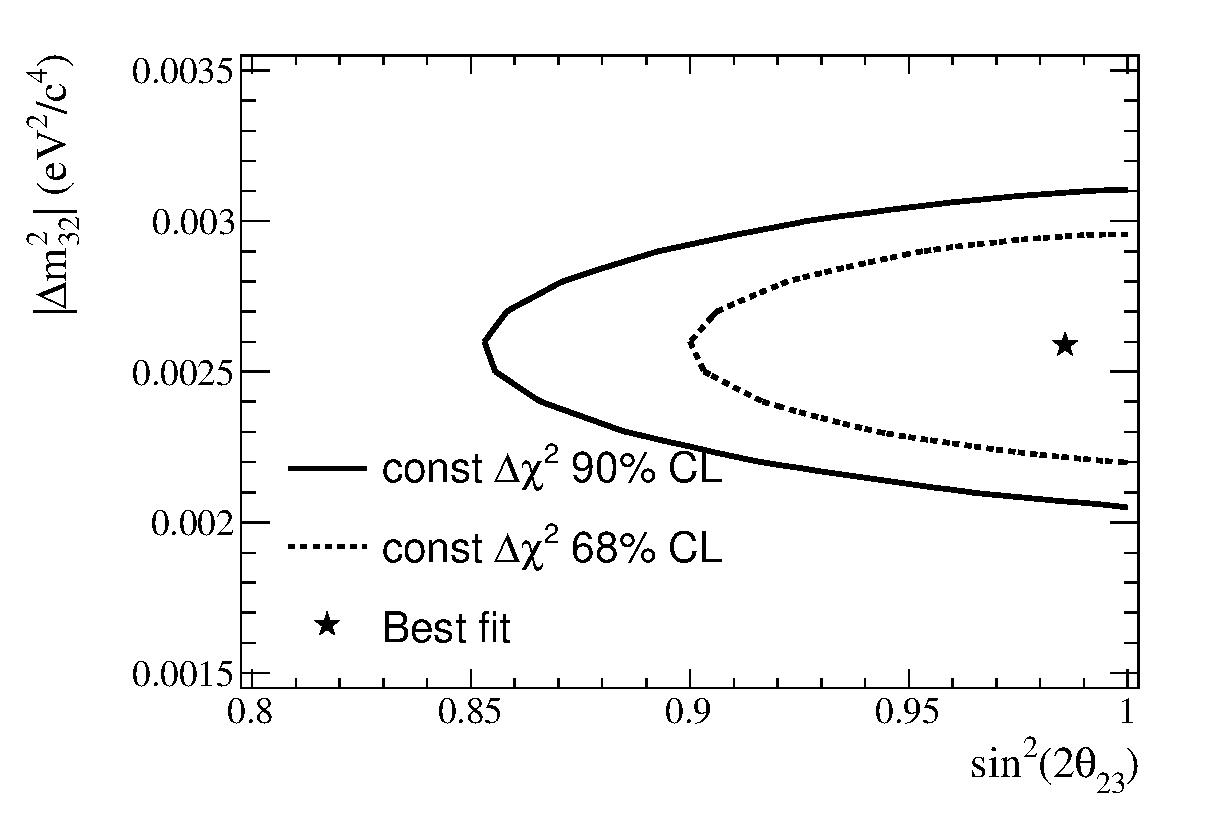
\includegraphics[width=20pc]{./images/fit_data/28/contours_4}
\caption {
  As in Fig.\ \ref{fig:results_data123_contour}, but for the Run 1+2 dataset only.
}
\label{fig:results_data12_contour}
\end{minipage}
\hspace{0.06\linewidth}
\begin{minipage}[t]{0.48\linewidth}
\center
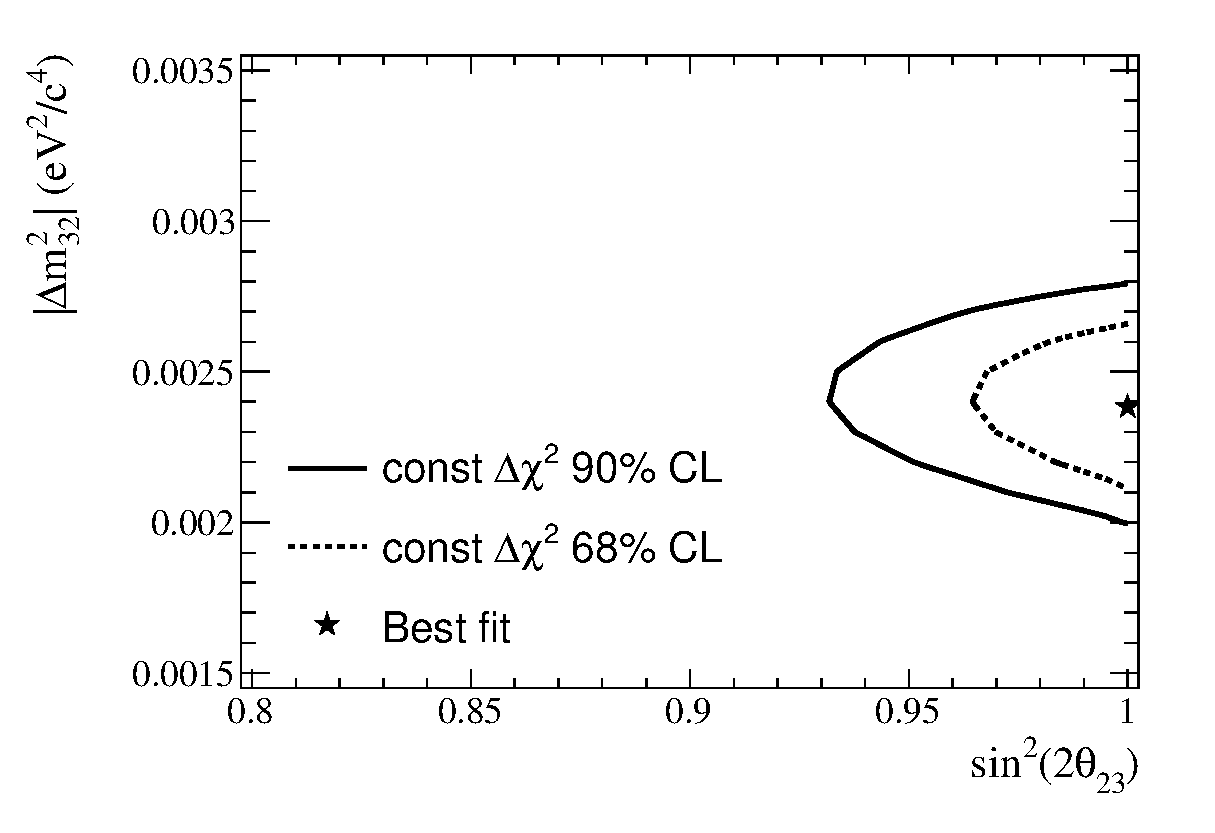
\includegraphics[width=20pc]{./images/fit_data/28/contours_5}
\caption {
  As in Fig.\ \ref{fig:results_data123_contour}, but for the Run 3 dataset only.
}
\label{fig:results_data3_contour}
\end{minipage}
\end{figure*}

%...........................................................
%
% FC contours for `2+N' fits
%

\begin{figure*}[htb]
\center
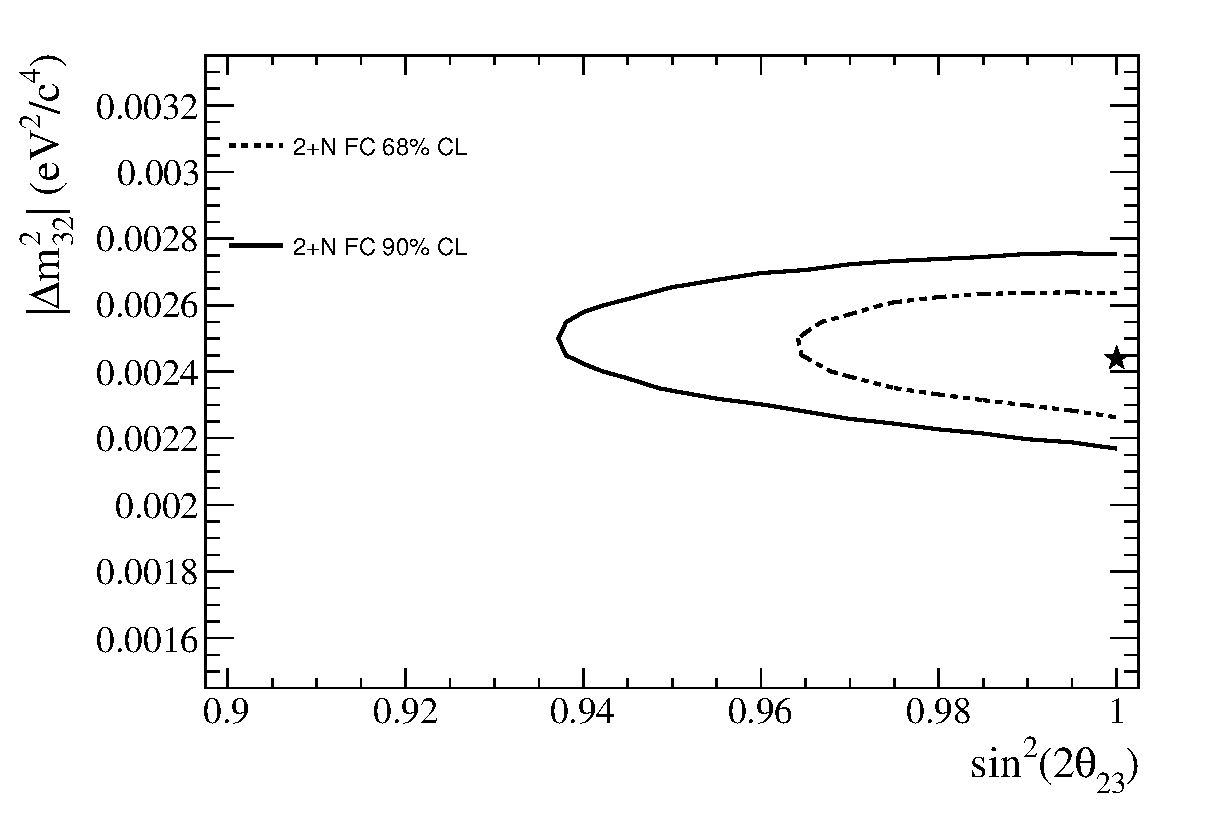
\includegraphics[width=35pc]{./images/fit_data/2N/2N_FC}
\caption {
  68\% CL and 90\% CL allowed region (including systematics), 
  constructed with the method of Feldman and Cousins,
  for the `2+N' fit to the Run 1+2+3 dataset assuming $\theta_{23}$ is in the first octant.
  The `2+N' best-fit point is also shown.
}
\label{fig:results_data123_fc_contour_2N}
\end{figure*}

\begin{figure*}[htb]
\center
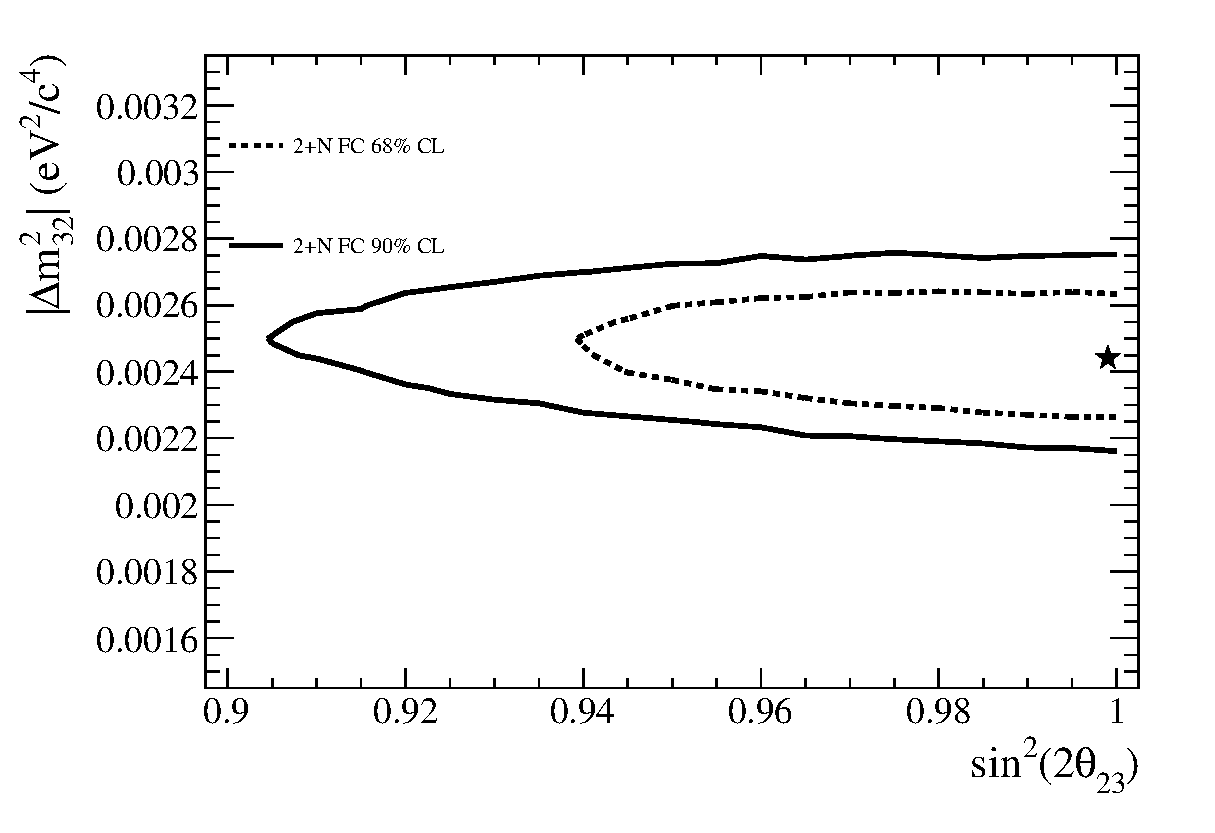
\includegraphics[width=35pc]{./images/fit_data/2Noctant2/2NO2_FC}
\caption {
  68\% CL and 90\% CL allowed region (including systematics), 
  constructed with the method of Feldman and Cousins,
  for the `2+N' fit to the Run 1+2+3 dataset assuming $\theta_{23}$ is in the second octant.
  The `2+N' best-fit point is also shown.
}
\label{fig:results_data123_fc_contour_2NO2}
\end{figure*}

%
%\begin{figure*}[htb]
%\begin{minipage}[t]{0.48\linewidth}
%\center
%
\includegraphics[width=20pc]{./images/placeholder}
%\caption {
%  As in Fig.\ \ref{fig:results_data123_fc_contour_2N}, but for the Run 1+2 dataset only.
%}
%\label{fig:results_data12_fc_contour_2N}
%\end{minipage}
%\hspace{0.06\linewidth}
%\begin{minipage}[t]{0.48\linewidth}
%\center
%
\includegraphics[width=20pc]{./images/placeholder}
%\caption {
%  As in Fig.\ \ref{fig:results_data123_fc_contour_2N}, but for the Run 3 dataset only.
%}
%\label{fig:results_data3_fc_contour_2N}
%\end{minipage}
%\end{figure*}
%

%...........................................................
%
% FC contours for `2+8' fits
%

\begin{figure*}[htb]
\center
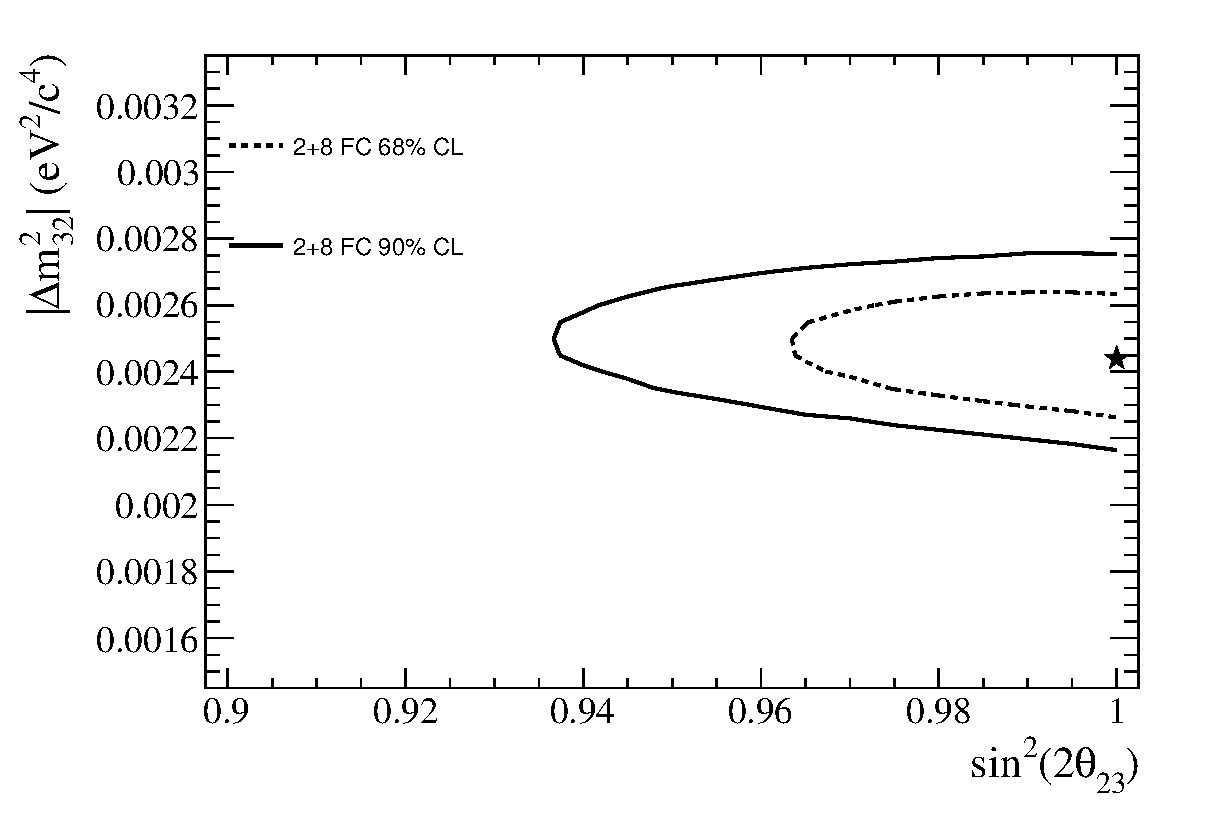
\includegraphics[width=35pc]{./images/fit_data/28/28_FC}
\caption {
  68\% CL and 90\% CL allowed region (including systematics), 
  constructed with the method of Feldman and Cousins,
  for the `2+8' fit to the Run 1+2+3 dataset.
  The `2+8' best-fit point is also shown.
}
\label{fig:results_data123_fc_contour}
\end{figure*}

%
%\begin{figure*}[htb]
%\begin{minipage}[t]{0.48\linewidth}
%\center
%
\includegraphics[width=20pc]{./images/placeholder}
%\caption {
%  As in Fig.\ \ref{fig:results_data123_fc_contour}, but for the Run 1+2 dataset only.
%}
%\label{fig:results_data12_fc_contour}
%\end{minipage}
%\hspace{0.06\linewidth}
%\begin{minipage}[t]{0.48\linewidth}
%\center
%
\includegraphics[width=20pc]{./images/placeholder}
%\caption {
%  As in Fig.\ \ref{fig:results_data123_fc_contour}, but for the Run 3 dataset only.
%}
%\label{fig:results_data3_fc_contour}
%\end{minipage}
%\end{figure*}
%

\clearpage

%--------------------------------------------------------------------------------------
% Contour comparisons
%--------------------------------------------------------------------------------------

\subsection {Confidence region comparisons}
\label{sec:results_contour_comparisons}


\subsubsection {Comparisons between the `2+N' contours assuming $\theta_{23}$ is in the first and second octants}

Comparisons were made between the allowed regions obtained using 
the different fits to the Run 1+2+3 dataset, 
A comparison between $\theta_{23}$ octant assumptions for the `2+N' regions 
constructed using the constant-$\Delta\chi^2$ method
is shown in Fig.\ \ref{fig:results_compare_contours_octants}.
A comparison between $\theta_{23}$ octant assumptions for the `2+N' regions 
constructed using the method of Feldman and Cousins
is shown in Fig.\ \ref{fig:results_compare_fc_contours_octants}.
The contours are visibly different; this is due to the next-to-leading order term in
Eq.\ \ref{eqn:numusurv3fapprox}.

Constant $\Delta\chi^2$ contours for both $\theta_{23}$ octant assumptions are converted
into $\sin^2\theta_{23}$-$|\Delta m^2_{32}|$ space in
Fig.\ \ref{fig:results_compare_contours_octants_sinsqtheta23}.
They are compared with the fit to $\sin^2\theta_{23}$.
% \footnote{
%   A fully validated fit to the Run 1+2+3 dataset using the VaLOR framework for $|\Delta m^2|$, $\sin^2\theta_{23}$ is presented
%   in \cite{OurRun123JointOscillationAnalysis}. The $\nu_\mu$ disappearance result from that note
%   is not shown here, due to that analysis using a different version of the BANFF matrix,
%   however it gives almost identical results.
% }.
The contours are identical, showing that the difference between contours from different $\theta_{23}$ octant
assumptions shown in Fig. \ref{fig:results_compare_contours_octants} is what is expected.
The best-fit values in $\sin^2\theta_{23}$ of the 3 fits are given in Tab.\ \ref{tab:bestfit_sinsqtheta}.

%......................................
% 2+N octants, const Delta\chisq method
%
\begin{figure*}[htb]
\center
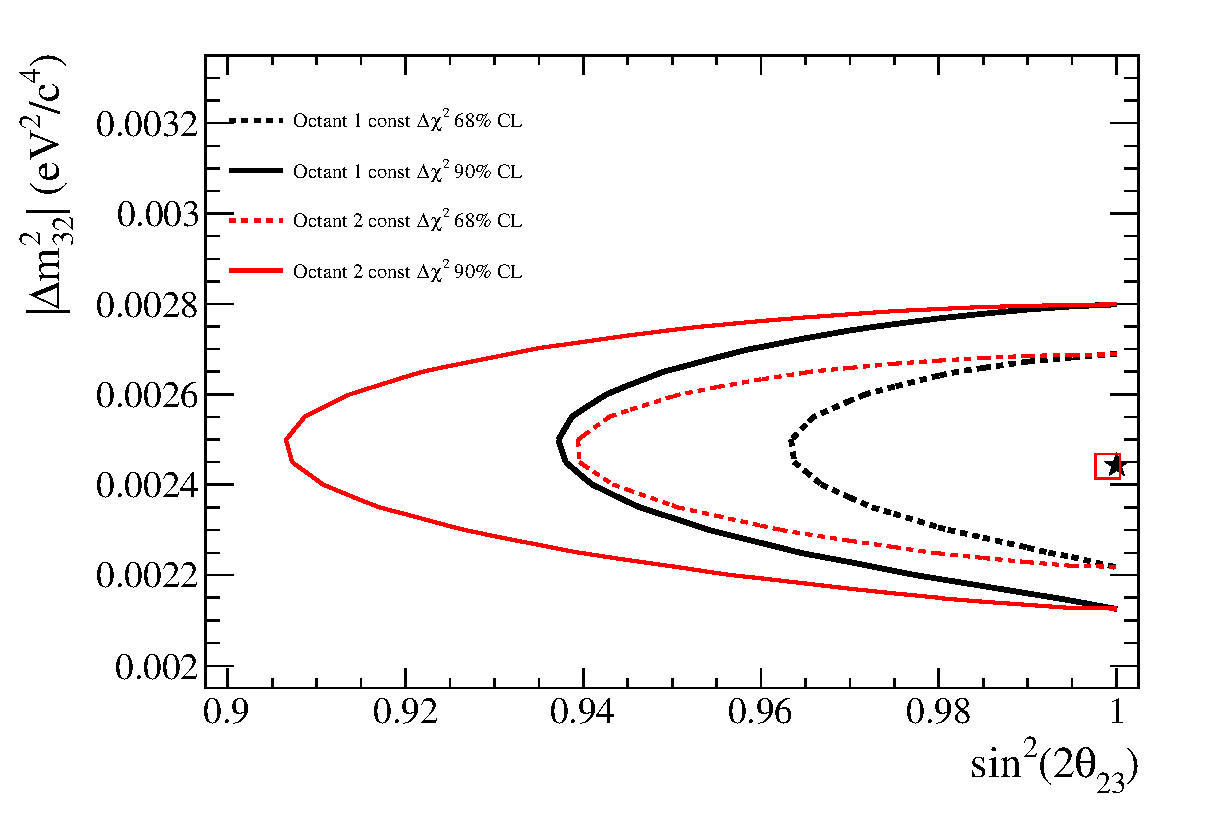
\includegraphics[width=35pc]{./images/fit_data/compare/compare_octants}
\caption {
  Comparison between the `2+N'
  68\% CL and 90\% CL allowed regions
  for $\theta_{23}$ in the first and second octants
  obtained using the constant-$\Delta\chi^2$ method. 
  The comparison is shown for the fits to the Run 1+2+3 dataset.
}
\label{fig:results_compare_contours_octants}
\end{figure*}

%......................................
% 2+N octants, FC method
%
\begin{figure*}[htb]
\center
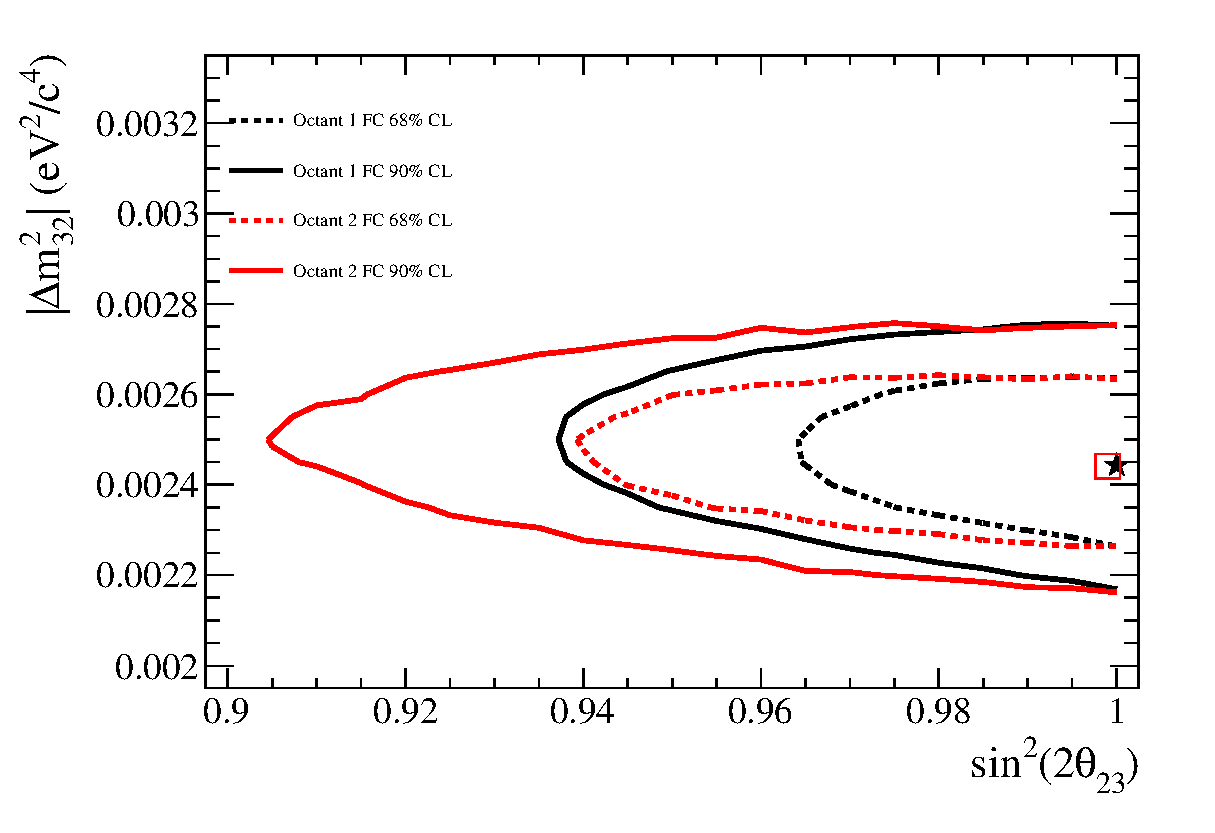
\includegraphics[width=35pc]{./images/fit_data/compare/compare_octants_FC}
\caption {
  Comparison between the `2+N'
  68\% CL and 90\% CL allowed regions
  for $\theta_{23}$ in the first and second octants
  obtained using the method of Feldman and Cousins.
  The comparison is shown for the fits to the Run 1+2+3 dataset.
}
\label{fig:results_compare_fc_contours_octants}
\end{figure*}

%......................................
% 2+N octants, converted into sinsqtheta23 space
%
\begin{figure*}[htb]
\center
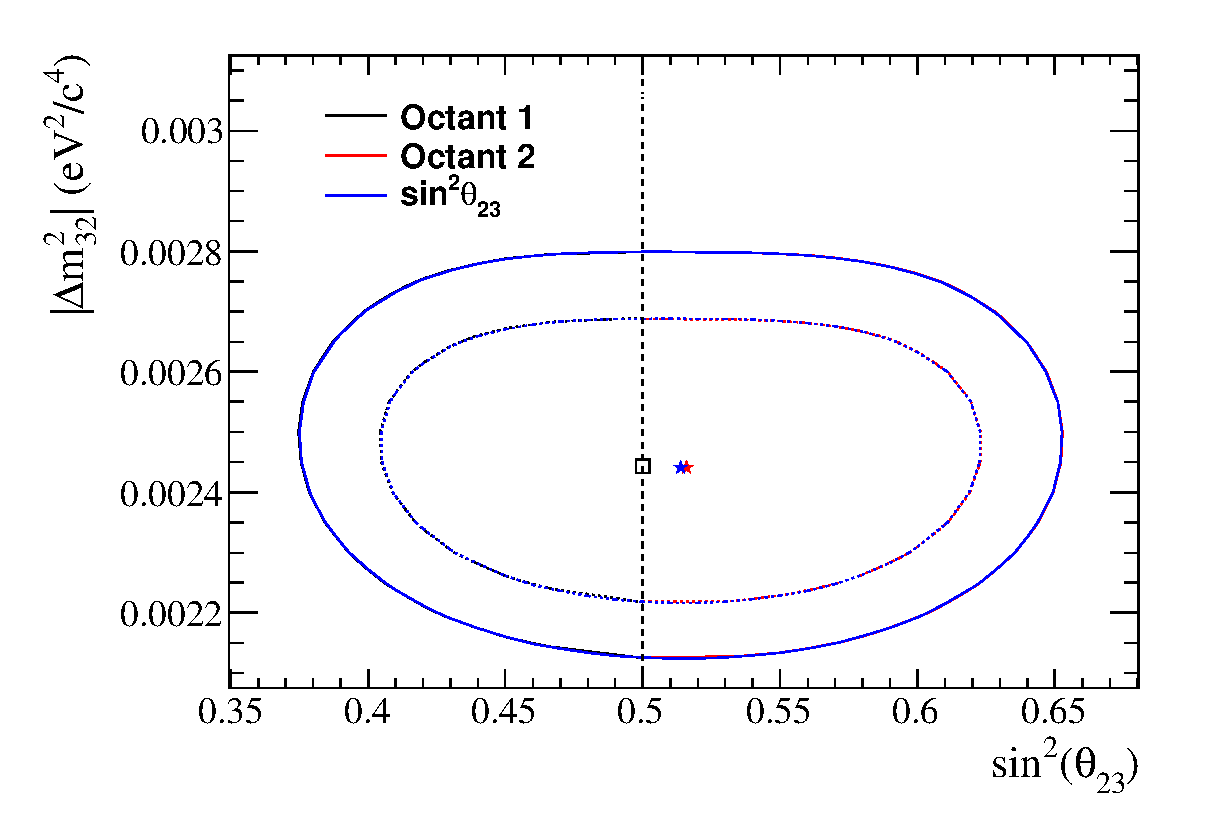
\includegraphics[width=35pc]{./images/fit_data/compare/contour_compare_octants_sinsqtheta}
\caption {
  Comparison between the `2+N'
  68\% CL and 90\% CL allowed regions
  for $\theta_{23}$ in the first and second octants
  obtained using the constant-$\Delta\chi^2$ method,
  and with the x-axis converted from $\sin^2 2 \theta_{23}$ to $\sin^2\theta_{23}$ after the fit.
  A '2+N' fit using $\sin^2\theta_{23}$ directly is also shown.
  The vertical line is the boundary between the octants to help guide the
  reader's eye.
  The comparison is shown for the fits to the Run 1+2+3 dataset.
}
\label{fig:results_compare_contours_octants_sinsqtheta23}
\end{figure*}

\clearpage

\subsubsection {Comparisons between the `2+N' and `2+8' contours}

Comparisons were made between the allowed regions obtained using 
the different fits to the Run 1+2+3 dataset, 
A comparison between the `2+N' and `2+8' regions 
constructed using the constant-$\Delta\chi^2$ method
is shown in Fig.\ \ref{fig:results_compare_contours_28_2N}.
A comparison between the `2+N' and `2+8' regions
constructed using the method of Feldman and Cousins
is shown in Fig.\ \ref{fig:results_compare_fc_contours_28_2N}.
For a given contour construction method,
the `2+N' and `2+8' contours are almost identical.

Fig.\ \ref{fig:results_compare_contours_28_2N_20} shows a comparison
between the `2+N' and `2+8' regions, constructed using the 
constant-$\Delta\chi^2$ method, with the corresponding results for `2+0'.
The `2+0' fit results in smaller contours.
The plot illustrates that, while with the present statistics fitting for 
systematics is warranted (`2+0' contours smaller than `2+8' and `2+N'),
the full effect of the systematics on the contour is encapsulated
by allowing only the the 8 dominant to float in the fit.

%......................................
% 2+N vs 2+8, const Delta\chisq method
%
\begin{figure*}[htb]
\center
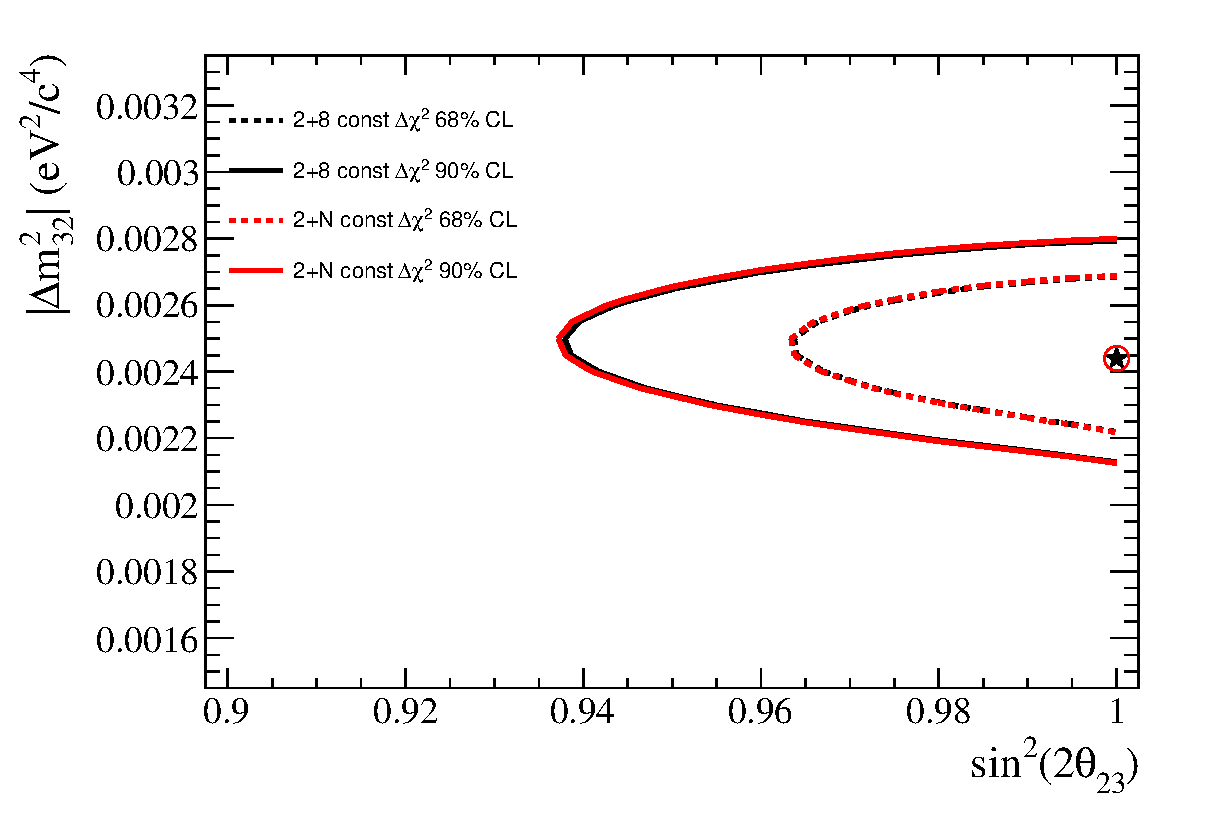
\includegraphics[width=35pc]{./images/fit_data/compare/compare_2all_28}
\caption {
  Comparison between the `2+N' and `2+8'
  68\% CL and 90\% CL allowed regions 
  obtained using the constant-$\Delta\chi^2$ method. 
  The comparison is shown for the fits to the Run 1+2+3 dataset.
  The `2+N' and `2+8' confidence regions are identical.
}
\label{fig:results_compare_contours_28_2N}
\end{figure*}

%......................................
% 2+N vs 2+8, FC method
%
\begin{figure*}[htb]
\center
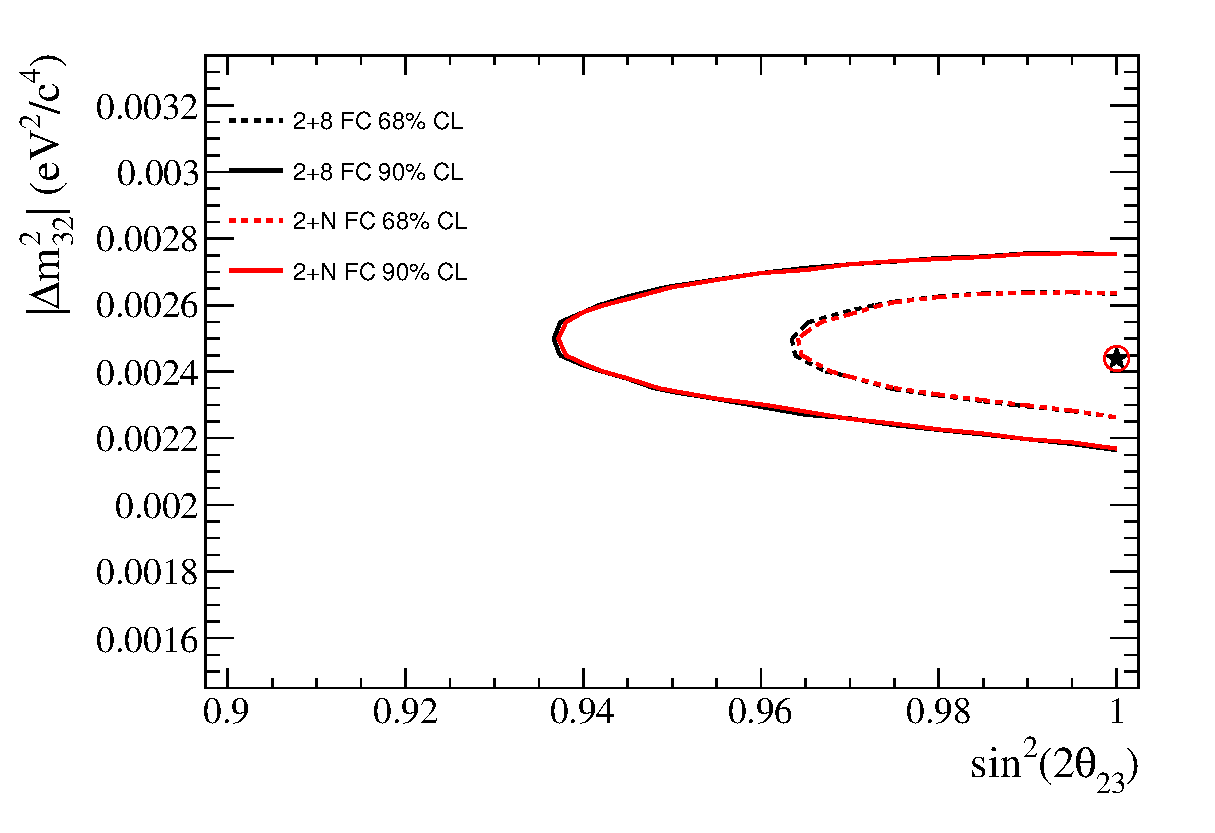
\includegraphics[width=35pc]{./images/fit_data/compare/compare_2all_28_FC}
\caption {
  Comparison between the `2+N' and `2+8'
  68\% CL and 90\% CL allowed regions
  obtained using the method of Feldman and Cousins.
  The comparison is shown for the fits to the Run 1+2+3 dataset.
}
\label{fig:results_compare_fc_contours_28_2N}
\end{figure*}

%......................................
% 2+N vs 2+8 vs 2+0, const Delta\chisq method
%
\begin{figure*}[htb]
\center
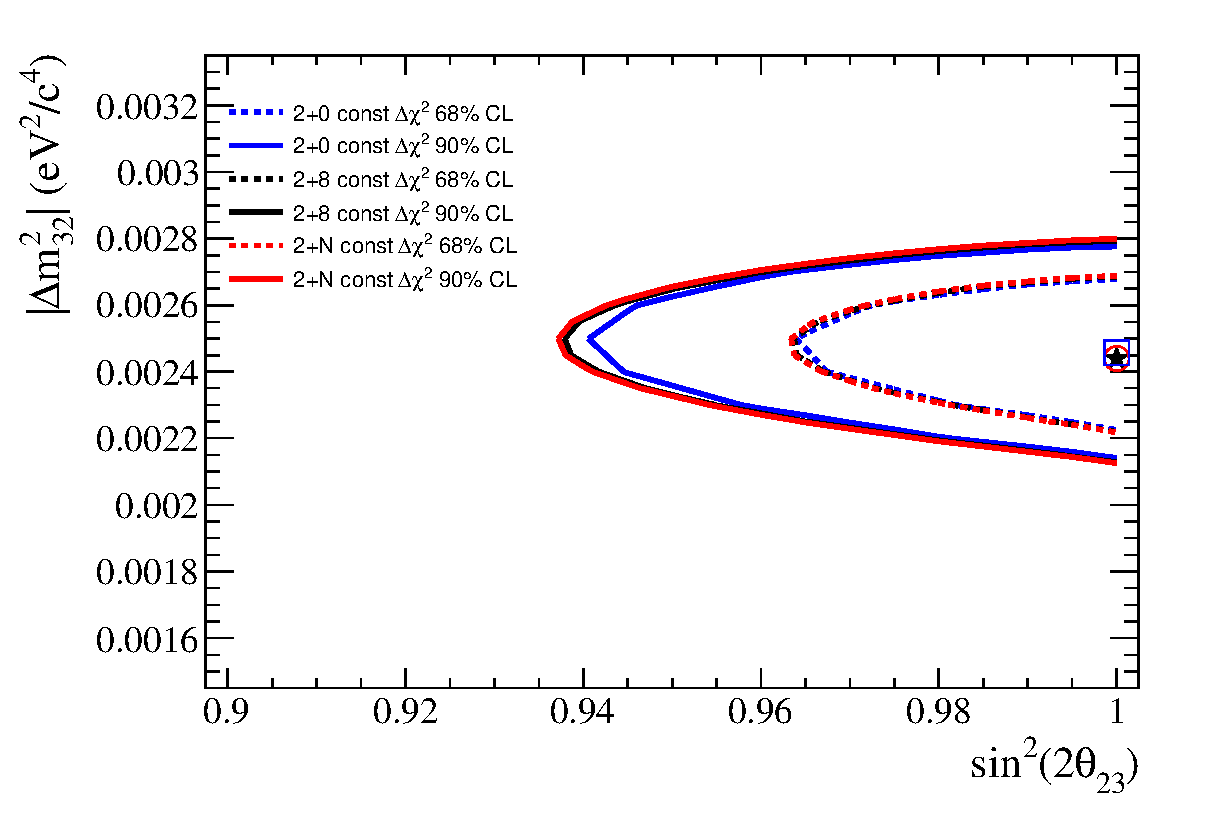
\includegraphics[width=35pc]{./images/fit_data/compare/compare_2all_28_20}
\caption {
  Comparison between the `2+N', `2+8' and `2+0'
  68\% CL and 90\% CL allowed regions 
  obtained using the constant-$\Delta\chi^2$ method. 
  The comparison is shown for the fits to the Run 1+2+3 dataset.
}
\label{fig:results_compare_contours_28_2N_20}
\end{figure*}

\clearpage

%......................................................................................
\subsubsection {Comparisons between the constant-$\Delta\chi^{2}$ and Feldman-Cousins contours}

The confidence regions obtained using the same fit variant 
but different contour construction methods were also compared.
In Fig.\ \ref{fig:results_compare_FC_constdchisq_2N}, 
a comparison between the contours obtained using the constant-$\Delta\chi^2$ and Feldman-Cousins methods
is shown for the `2+N' fit to the Run 1+2+3 dataset.
In Fig.\ \ref{fig:results_compare_FC_constdchisq_2NO2}, 
the same comparison is shown for the `2+N' fit assuming $\theta_{23}$ is in the second octant.
In Fig.\ \ref{fig:results_compare_FC_constdchisq}, 
the same comparison is shown for the `2+8' fit.

%......................
%
% const Delta\chisq vs FC, 2+N
%
\begin{figure*}[htb]
\center
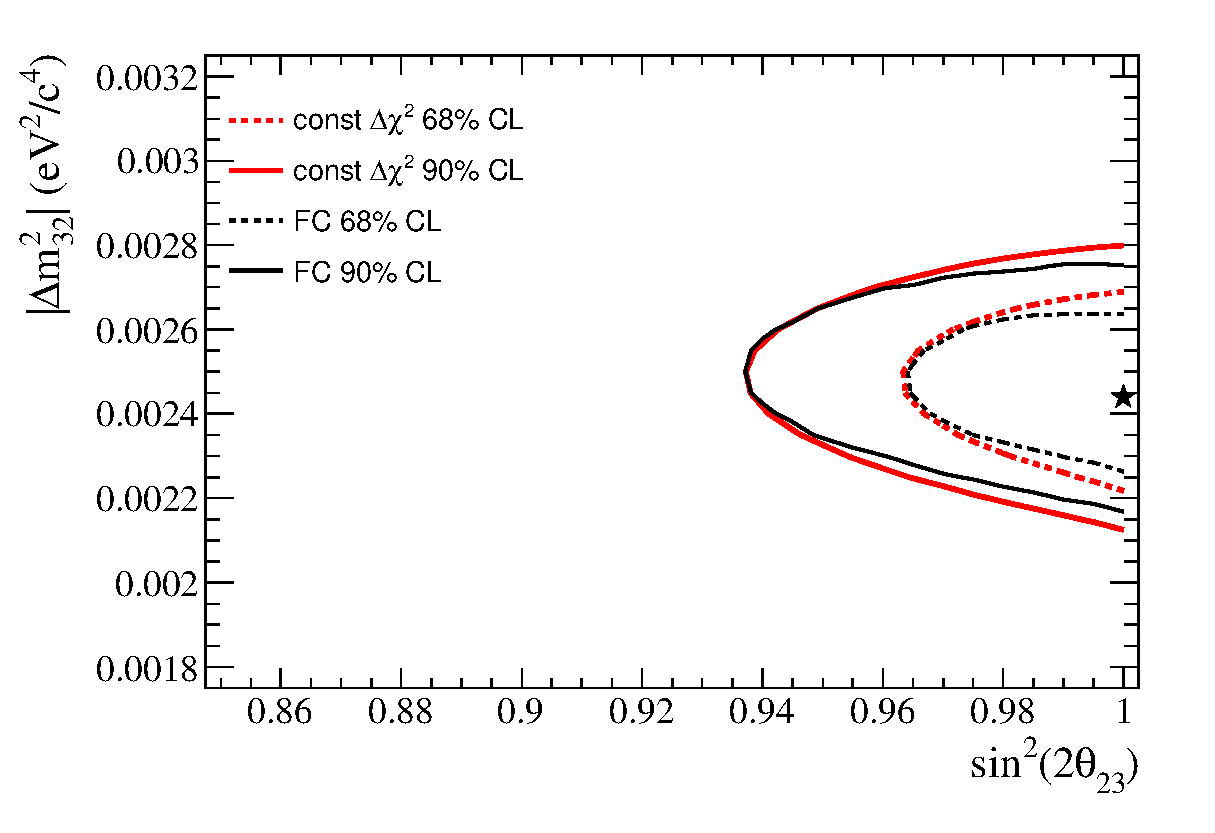
\includegraphics[width=30pc]{./images/fit_data/compare/compare_FC_constchisq_2N}
\caption {
  Comparison between the 68\% CL and 90\% CL allowed regions 
  obtained using the constant-$\Delta\chi^2$ and Feldman-Cousins methods 
  for the `2+N' fit to the Run 1+2+3 dataset assuming $\theta_{23}$ is in the first octant.
}
\label{fig:results_compare_FC_constdchisq_2N}
\end{figure*}


%......................
%
% const Delta\chisq vs FC, 2+N, second octant
%
\begin{figure*}[htb]
\center
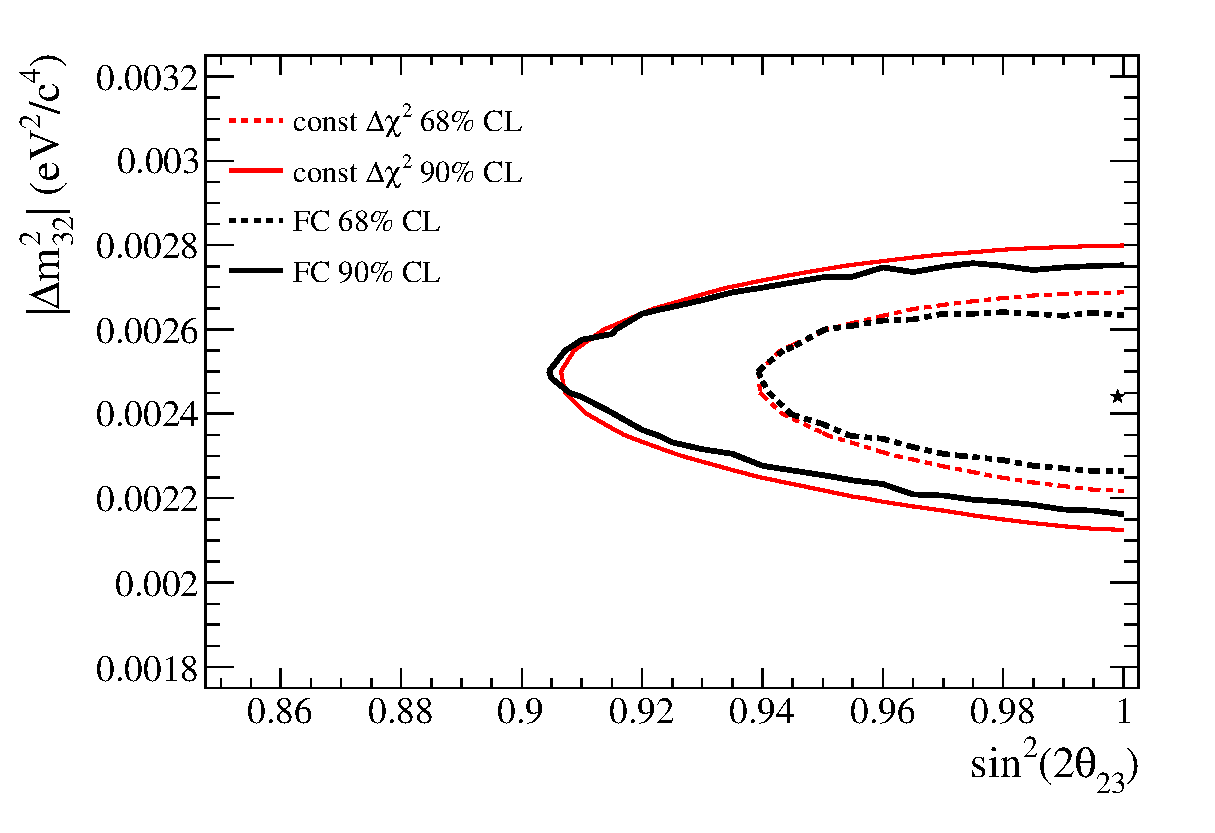
\includegraphics[width=30pc]{./images/fit_data/compare/compare_FC_constchisq_2NO2}
\caption {
  Comparison between the 68\% CL and 90\% CL allowed regions 
  obtained using the constant-$\Delta\chi^2$ and Feldman-Cousins methods 
  for the `2+N' fit to the Run 1+2+3 dataset assuming $\theta_{23}$ is in the second octant.
}
\label{fig:results_compare_FC_constdchisq_2NO2}
\end{figure*}


%......................
%
% const Delta\chisq vs FC, 2+8
%
\begin{figure*}[htb]
\center
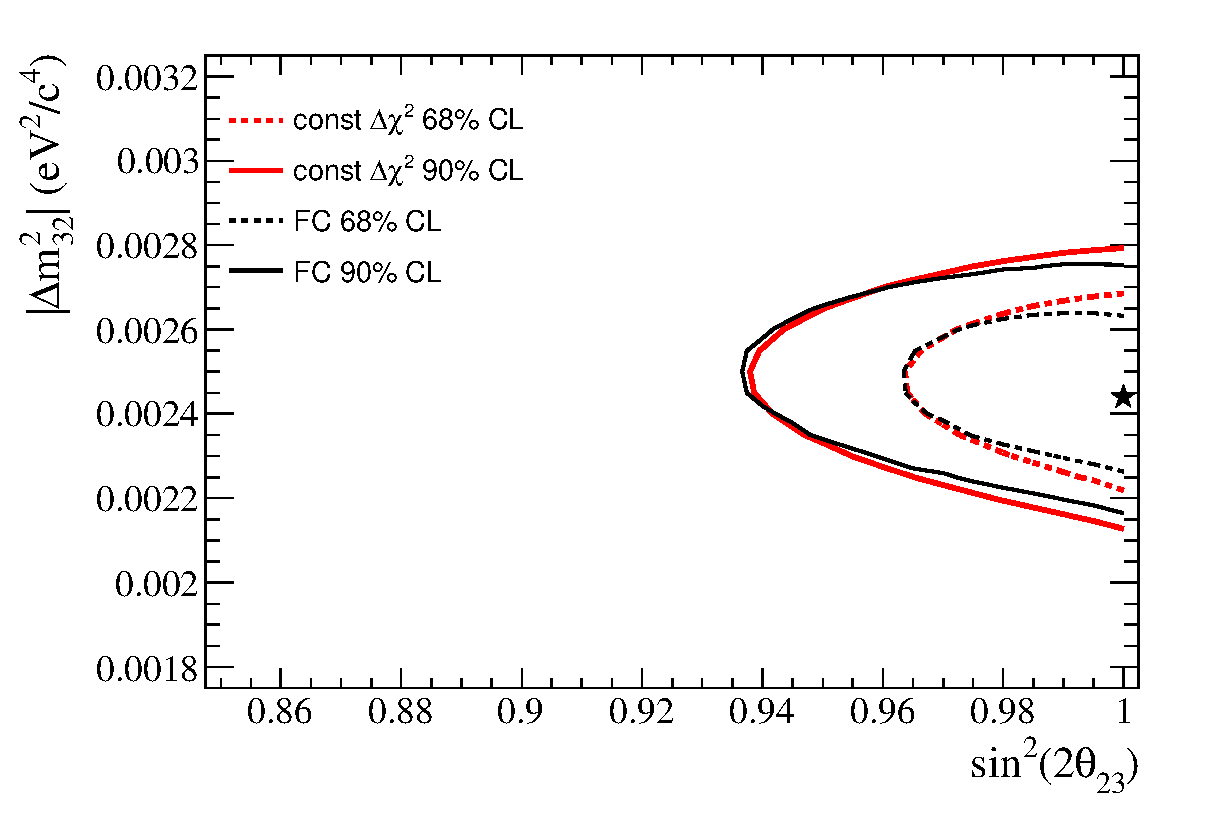
\includegraphics[width=30pc]{./images/fit_data/compare/compare_FC_constchisq}
\caption {
  Comparison between the 68\% CL and 90\% CL allowed regions 
  obtained using the constant-$\Delta\chi^2$ and Feldman-Cousins methods 
  for the `2+8' fit to the Run 1+2+3 dataset.
}
\label{fig:results_compare_FC_constdchisq}
\end{figure*}

\clearpage

%......................................................................................
\subsubsection {Comparisons with recent measurements from MINOS and SuperK}

Comparisons were produced between our Run 1+2+3 results and the updated results from 
MINOS 2013 (3-flavour analysis) \cite{MINOS2013:3nu} and SuperK 2012 atmospherics (3-flavour 
zenith-angle analysis) \cite{SKAtm2012}.
The comparison is shown 
in Fig.\ \ref{fig:results_compare_FC_constdchisq_external_2Nsintheta} for the `2+N' fit for $\sin^2\theta_{23}$.

Comparisons were produced between our Run 1+2+3 results and the updated (2012) results from 
MINOS \cite{MINOS2012} and SuperK atmospherics (both the 2-flavour L/E and 3-flavour 
zenith-angle analyses) \cite{SKAtm2012}.
The comparison is shown 
in Fig.\ \ref{fig:results_compare_FC_constdchisq_external_2N} for the `2+N' fit assuming $\theta_{23}$ is in the first octant,
in Fig.\ \ref{fig:results_compare_FC_constdchisq_external_2NO2} for the `2+N' fit assuming it is in the second octant, and
in Fig.\ \ref{fig:results_compare_FC_constdchisq_external} for the `2+8' fit.
A comparison of '2+N' FC contours with the external data is shown in Fig.\ \ref{fig:results_compare_FC_octants}
for both octant assumptions.

%......................
%
% VaLOR vs the world, 2+N sintheta
%
\begin{figure*}[htb]
\center
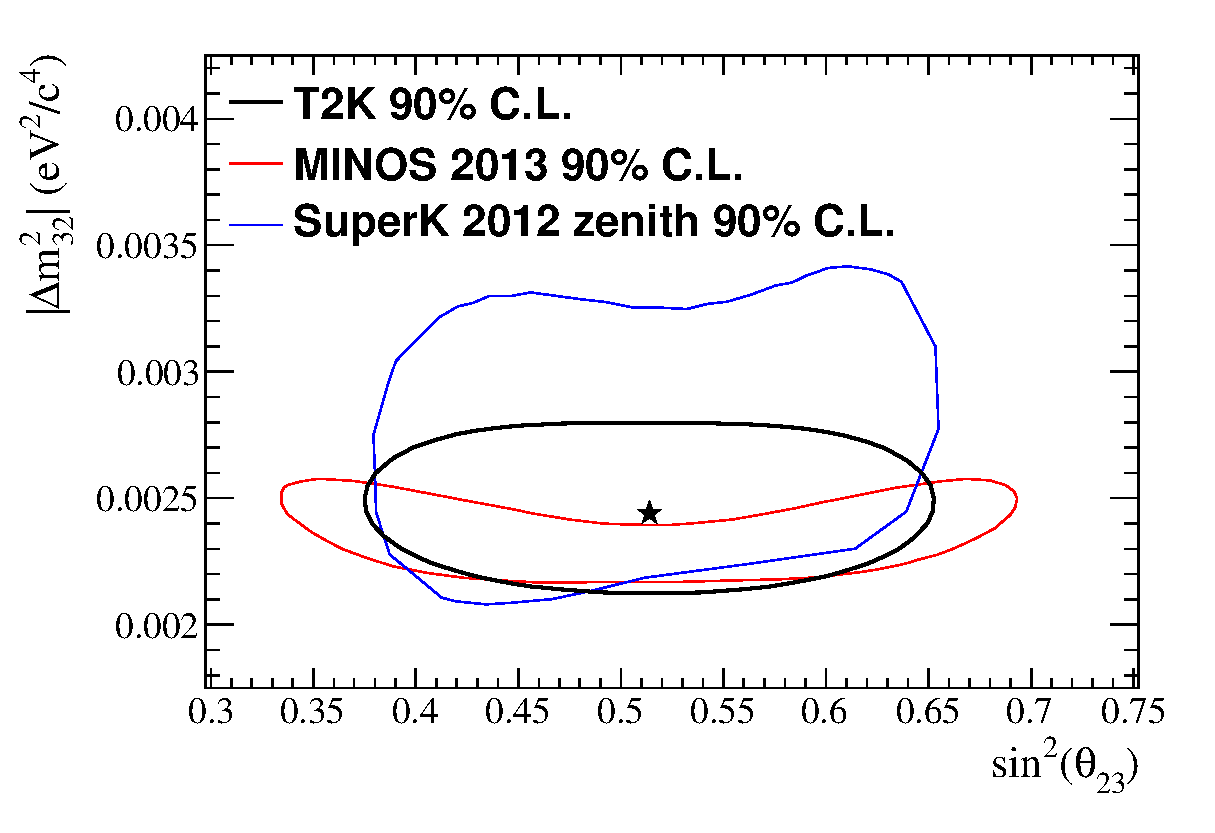
\includegraphics[width=30pc]{./images/fit_data/compare/compare_contours_external_sintheta}
\caption {
  Comparison between 90\% CL allowed regions 
  from MINOS \cite{MINOS2013:3nu} and SuperK atmospherics \cite{SKAtm2012},
  and the 90\% CL region obtained from the VaLOR `2+N' $\sin^2\theta_{23}$ fit to the Run 1+2+3 dataset,
  using the constant-$\Delta\chi^2$ method.
}
\label{fig:results_compare_FC_constdchisq_external_2Nsintheta}
\end{figure*}

%......................
%
% VaLOR vs the world, 2+N
%
\begin{figure*}[htb]
\center
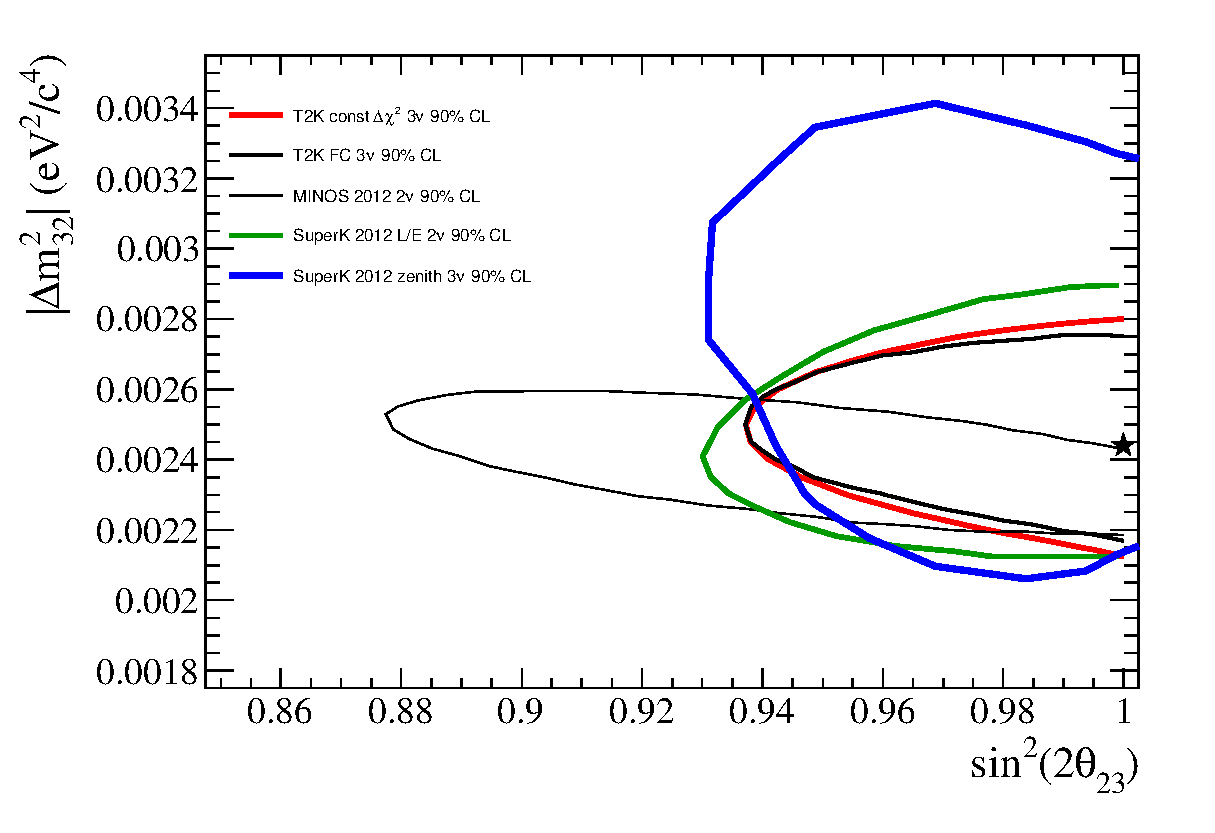
\includegraphics[width=30pc]{./images/fit_data/compare/compare_FC_constchisq_external_2N}
\caption {
  Comparison between 90\% CL allowed regions 
  from MINOS \cite{MINOS2012} and SuperK atmospherics \cite{SKAtm2012},
  and the 90\% CL regions obtained from the VaLOR `2+N' fit to the Run 1+2+3 dataset.
  Contours obtained using both the constant-$\Delta\chi^2$ and Feldman-Cousins methods are shown.
}
\label{fig:results_compare_FC_constdchisq_external_2N}
\end{figure*}

%......................
%
% VaLOR vs the world, 2+N, second octant
%
\begin{figure*}[htb]
\center
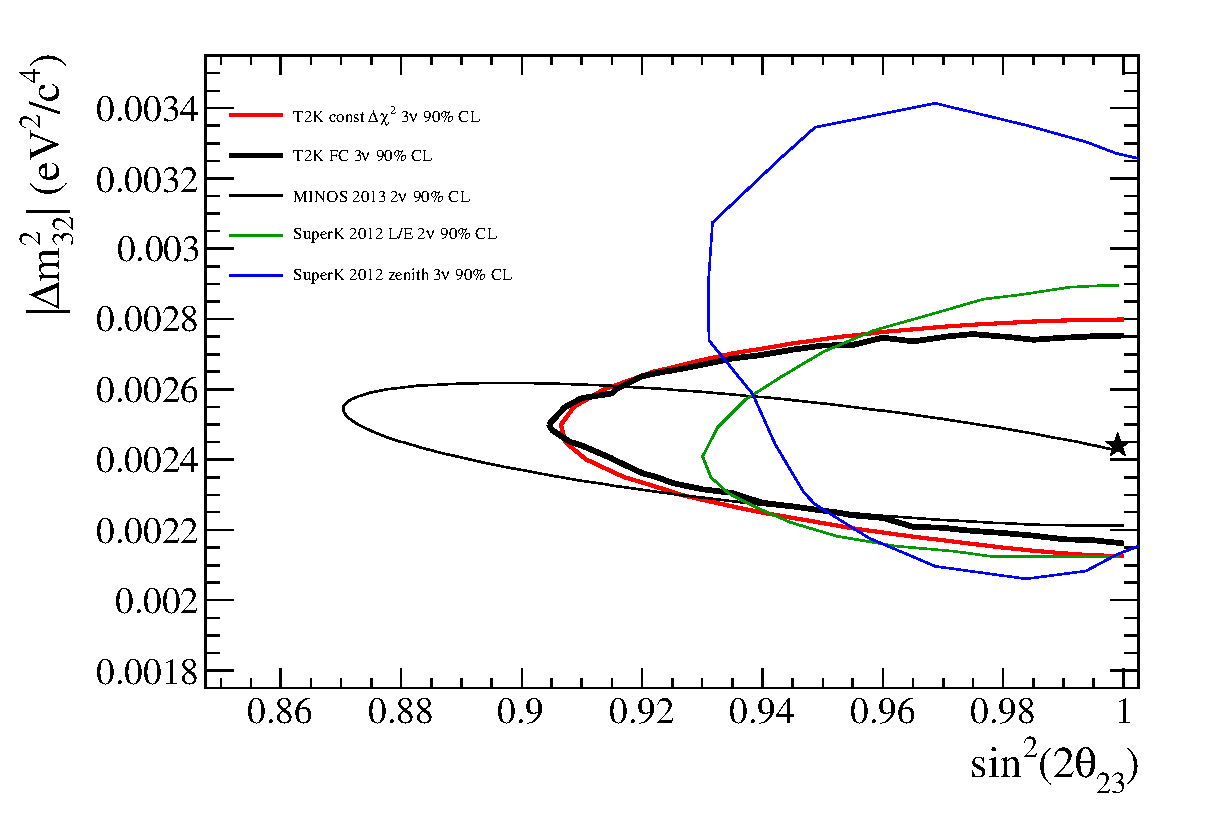
\includegraphics[width=30pc]{./images/fit_data/compare/compare_FC_constchisq_external_2NO2}
\caption {
  As in Fig.\ \ref{fig:results_compare_FC_constdchisq_external_2N}, but for the `2+N' fit assuming $\theta_{23}$ is in the second octant.
}
\label{fig:results_compare_FC_constdchisq_external_2NO2}
\end{figure*}

%......................
%
% VaLOR vs the world, 2+8
%
\begin{figure*}[htb]
\center
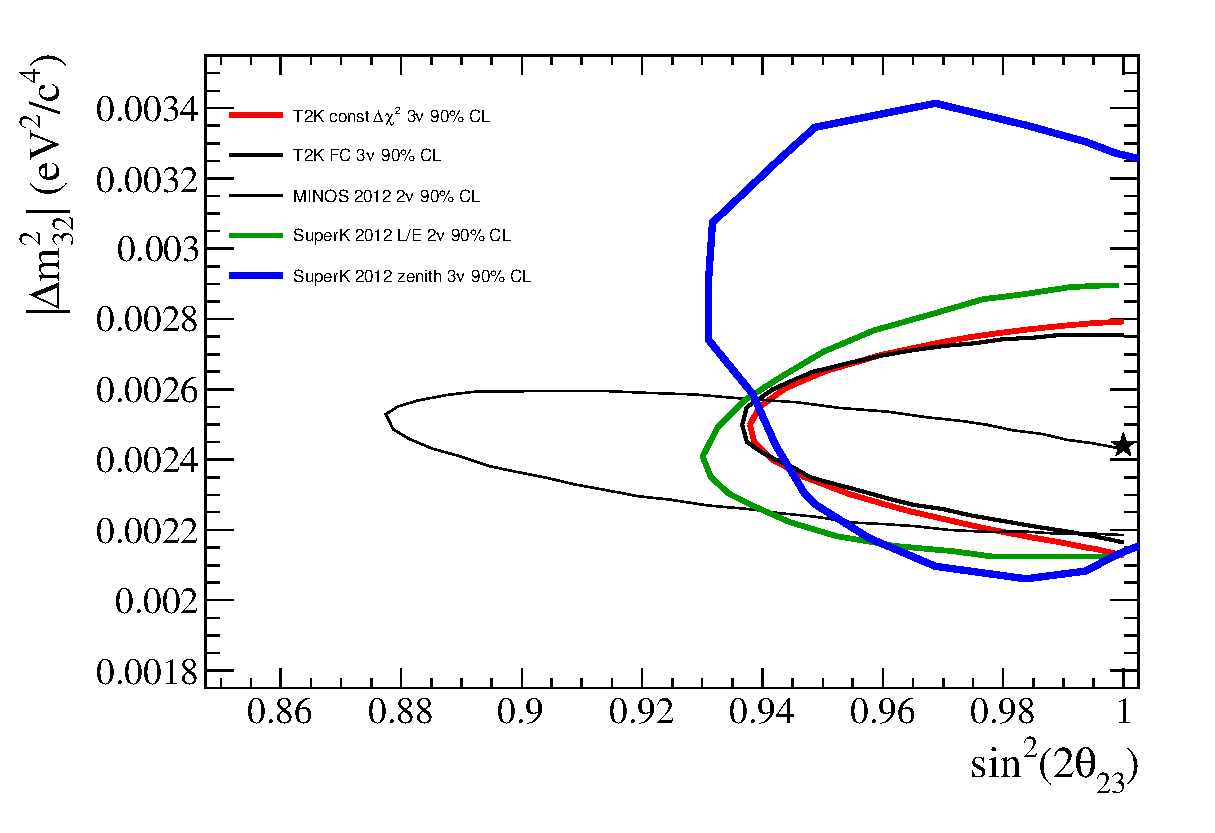
\includegraphics[width=30pc]{./images/fit_data/compare/compare_FC_constchisq_external}
\caption {
  As in Fig.\ \ref{fig:results_compare_FC_constdchisq_external_2N}, but for the `2+8' fit.
}
\label{fig:results_compare_FC_constdchisq_external}
\end{figure*}

%......................
%
% VaLOR vs the world, 2+N, FC, both octants
%
\begin{figure*}[htb]
\center
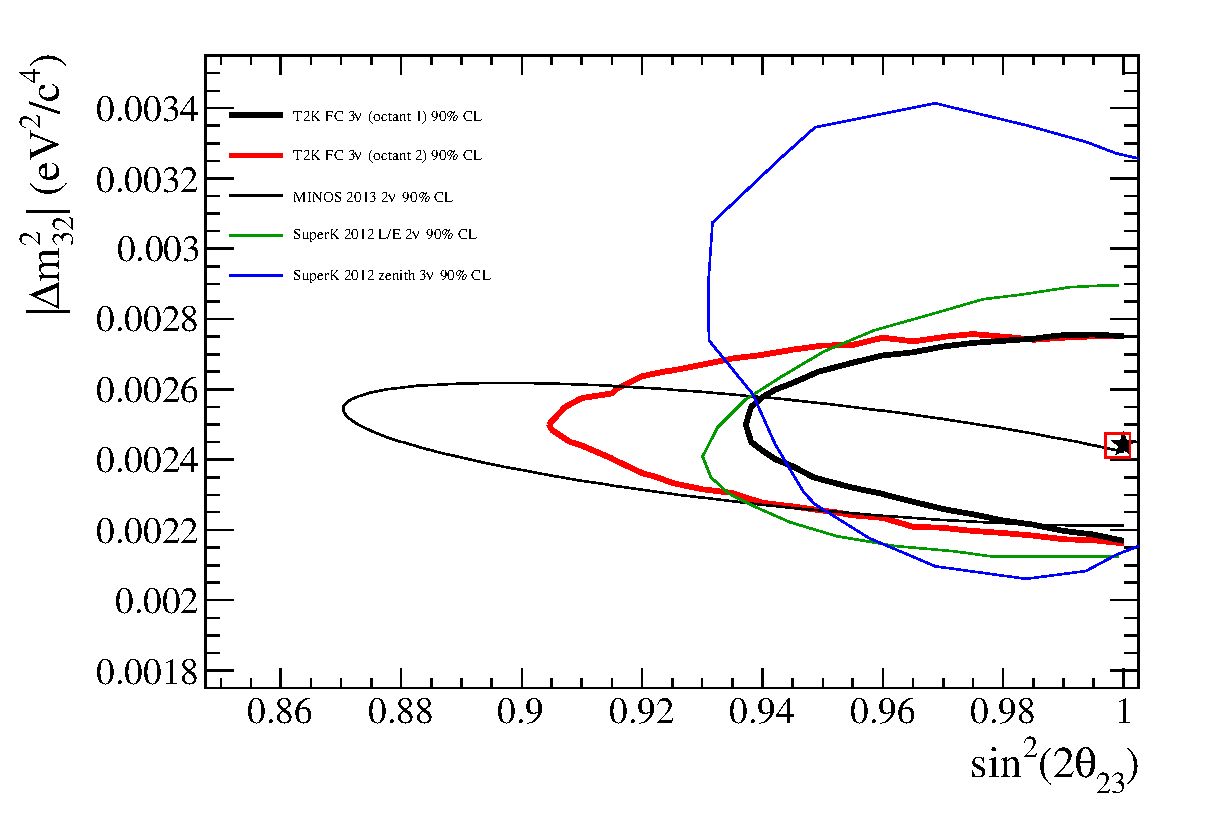
\includegraphics[width=30pc]{./images/fit_data/compare/compare_FC_octants_external}
\caption {
  Comparison between 90\% CL allowed regions 
  from MINOS \cite{MINOS2012} and SuperK atmospherics \cite{SKAtm2012},
  and the 90\% CL regions obtained from the VaLOR `2+N' fit to the Run 1+2+3 dataset.
  Contours obtained using both $\theta_{23}$ octant assumptions are shown.
}
\label{fig:results_compare_FC_octants}
\end{figure*}


\clearpage

%......................................................................................
\subsubsection {Comparisons with sensitivity}

In Fig.\ \ref{fig:results_compare_28_constdchisq_sensitivity}, 
a comparison is shown
between the Run 1+2+3 allowed regions obtained using the `2+8' fit and the
constant-$\Delta\chi^{2}$ method, and the T2K 3.010$\times$10$^{20}$ POT sensitivity
contours produced at the `2+8' best-fit point for the Run 1+2+3 dataset.
The sensitivity contours were computed by averaging the contours of 1k toy-MC
experiments generated with statistical fluctations and all systematic parameters randomized.
The plot indicates that the Run 1+2+3 dataset, is a ``favourable'' fluctuation
allowing us to quote confidence regions which are more restrictive than 
those that would be expected given our sensitivity.
This favourable fluctuation is not unlikely as shown 
in Fig.\ \ref{fig:results_compare_28_constdchisq_sensitivity_exclusion}.

%......................
%
\begin{figure*}[htb]
\center
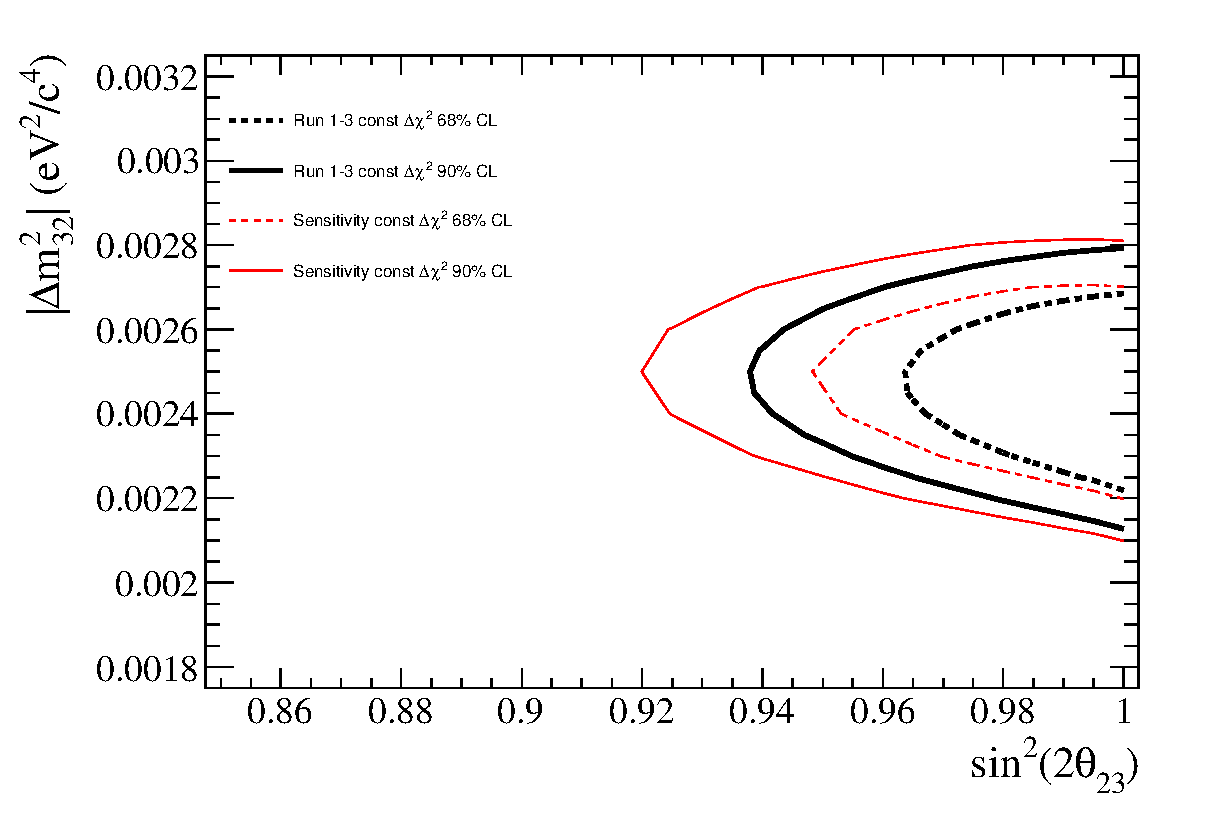
\includegraphics[width=30pc]{./images/fit_data/compare/compare_constchisq_sensitivity}
\caption {
  Comparison between the 68\% CL and 90\% CL allowed regions using the constant-$\Delta\chi^2$ 
  method for the `2+8' fit to the Run 1+2+3 dataset
  and the result of a sensitivity study at the `2+8' best-fit point for Run 1+2+3.
}
\label{fig:results_compare_28_constdchisq_sensitivity}
\end{figure*}

%......................
%
\begin{figure*}[htb]
\center
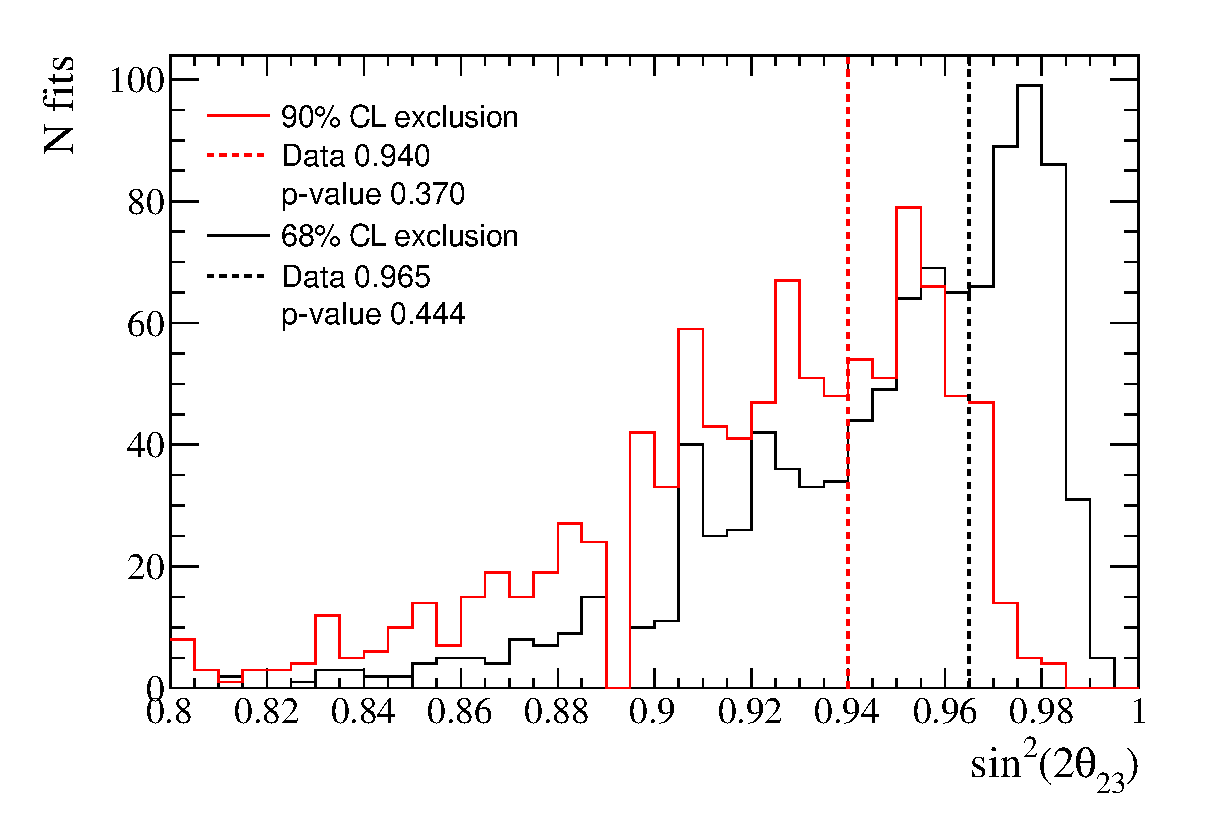
\includegraphics[width=25pc]{./images/sensitivities/2+8constdchisq/sensitivity_exclusion}
\caption {
  Distribution of minimum excluded value of sin$^22\theta_{23}$, for both 68\% CL and 90\% CL.
  The dashed lines show the minimum excluded value for the `2+8' fit
  to the Run 1+2+3 dataset, using the constant-$\Delta \chi^2$ method  
  (68\% CL in black and 90\% CL in red).  
}
\label{fig:results_compare_28_constdchisq_sensitivity_exclusion}
\end{figure*}


\clearpage

%......................................................................................
%\subsubsection {Comparison between the 2012 and 2010 analyses}
%
%Fig. \ref{fig:results_compare_2010_2012}
%
%The
%%......................
%%
%\begin{figure*}[htb]
%\center
%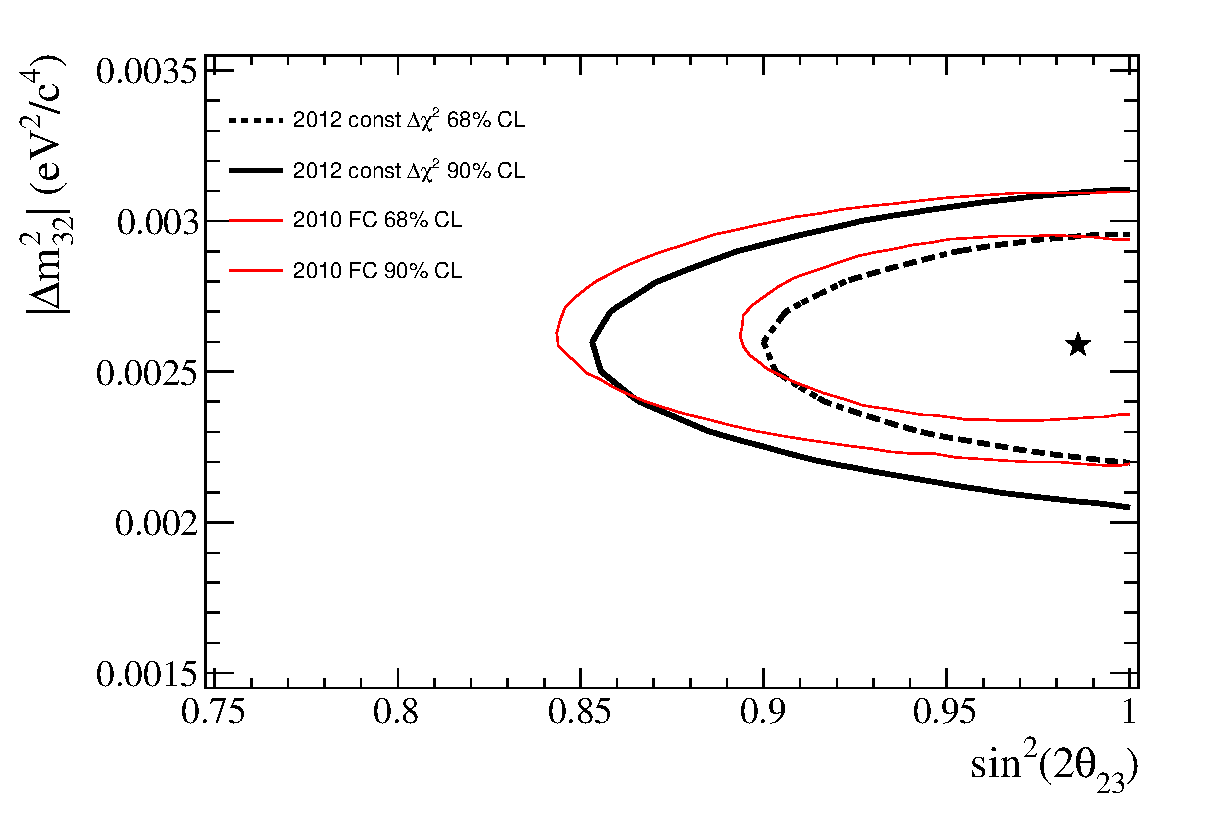
\includegraphics[width=35pc]{./images/fit_data/compare/compare_run12_2012_2010}
%\caption {
%  Comparison of 68\% CL and 90\% CL allowed regions of 2010 and 2012 methods, in a fit to Run I+II data.
%  The 2012 result shown used the 2+8 constant-$\Delta\chi^2$ method.
%  The 2010 result is taken from \cite{OurRun12DisappAnalysis}.
%}
%\label{fig:results_compare_2010_2012}
%\end{figure*}
%
%
%......................................................................................

\subsubsection {Comparisons of individual run periods}

A comparison between the confidence regions obtained by three 
separate `2+N' analyses of the Run 1+2+3, Run 1+2 and Run 3 datasets 
is shown in Fig.\ \ref{fig:results_compare_runs_2N}.
The corresponding plot for the `2+8' fit  
is shown in Fig.\ \ref{fig:results_compare_runs}.
The contours from the different running periods are consistent.

%......................
%
% Run1+2+3 vs Run1+2 vs Run3, 2+N
%
\begin{figure*}[htb]
\center
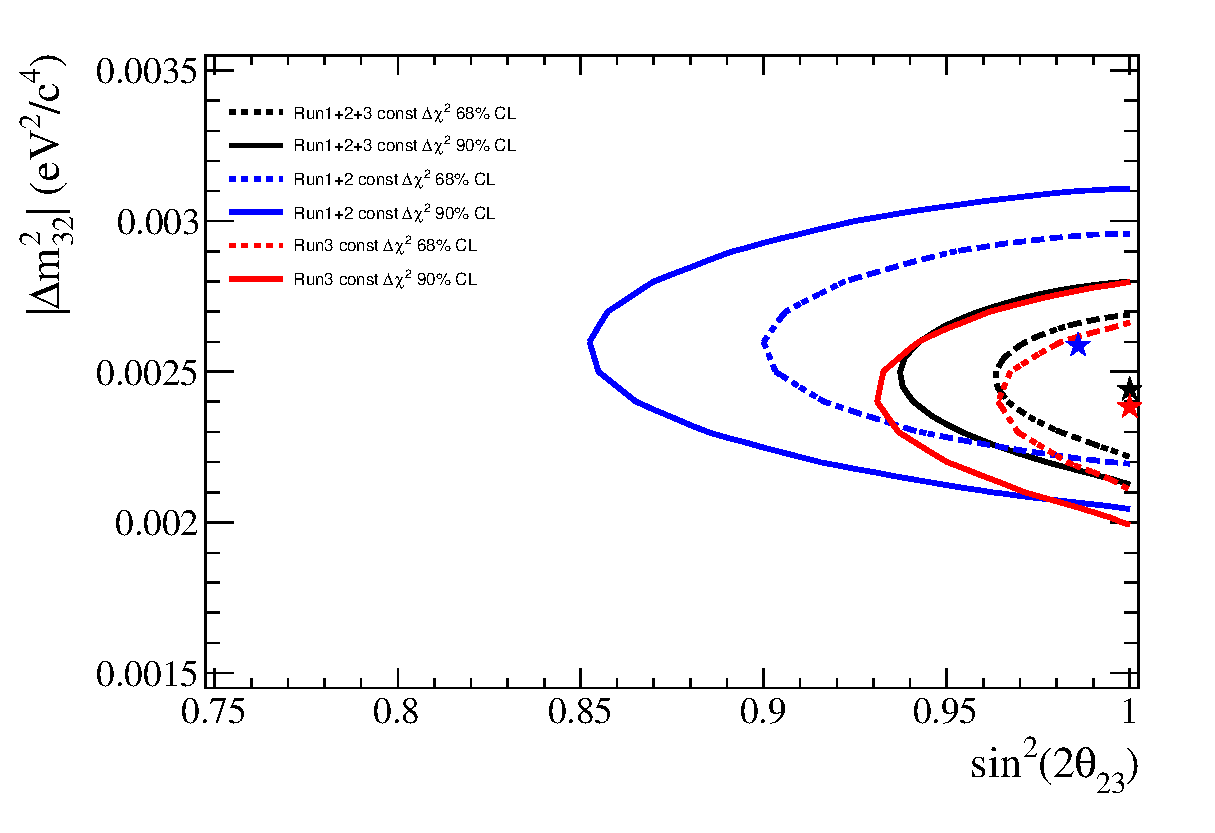
\includegraphics[width=30pc]{./images/fit_data/compare/compare_runs_2N}
\caption {
  Comparison between the 68\% CL and 90\% CL allowed regions obtained from separate
  `2+N' analyses of the Run 1+2+3, Run 1+2 and Run 3 datasets.
  All contours shown were calculated with the constant-$\Delta\chi^2$ method.
}
\label{fig:results_compare_runs_2N}
\end{figure*}

%......................
%
% Run1+2+3 vs Run1+2 vs Run3, 2+8
%
\begin{figure*}[htb]
\center
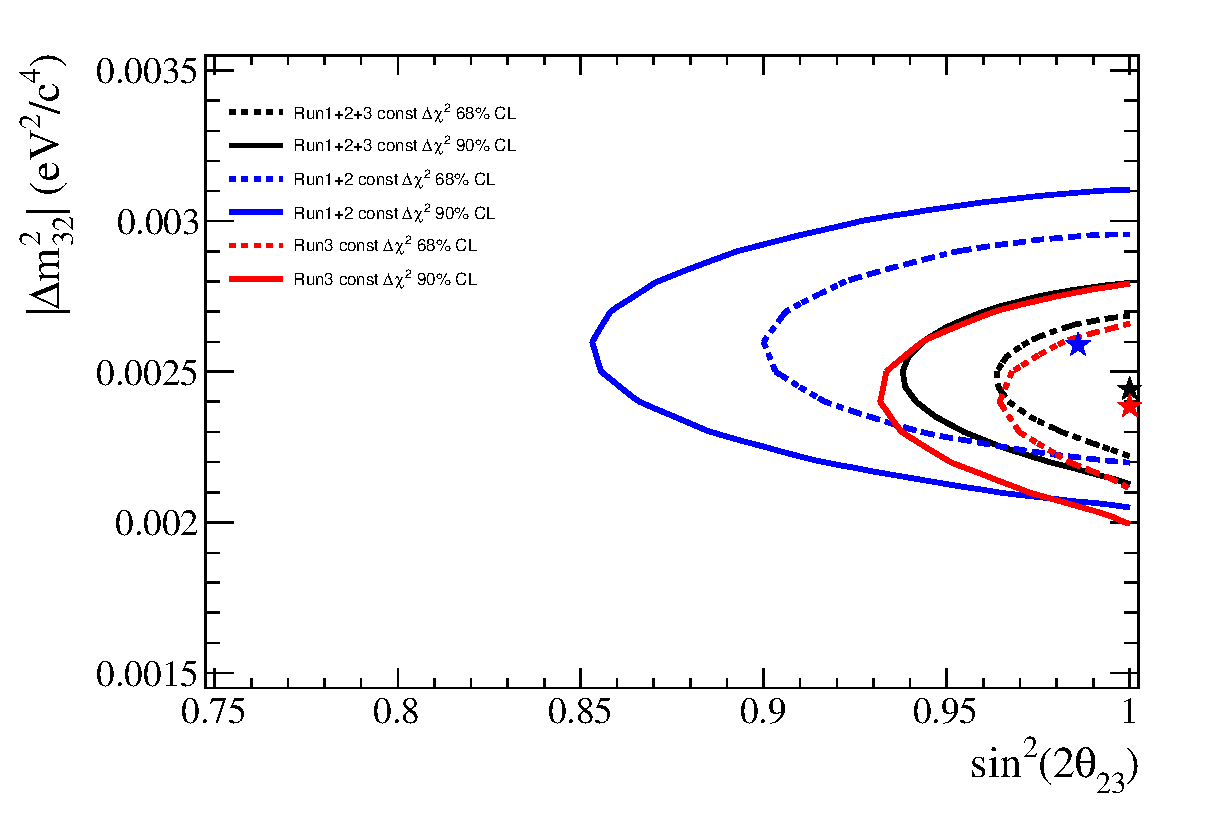
\includegraphics[width=30pc]{./images/fit_data/compare/compare_runs}
\caption {
  Comparison between the 68\% CL and 90\% CL allowed regions obtained from separate
  `2+8' analyses of the Run 1+2+3, Run 1+2 and Run 3 datasets.
  All contours shown were calculated with the constant-$\Delta\chi^2$ method.
}
\label{fig:results_compare_runs}
\end{figure*}


\clearpage

%--------------------------------------------------------------------------------------
% Our views
%--------------------------------------------------------------------------------------

\subsection {The VaLOR group perspective on the choice of primary result}
\label{sec:primary_result_selection}

Four separate $\nu_{\mu}$-disappearance results have been produced by this analysis
for the Run 1+2+3 dataset; this is because we have used two fitting methods 
(`2+N' and `2+8') and two methods for constructing confidence regions (constant-$\Delta\chi^{2}$ 
and Feldman-Cousins).

This analysis used contours produced with the constant-$\Delta\chi^{2}$ method quite extensively, 
especially during its development and for the sensitivity studies. We considered that producing Feldman-Cousins 
contours at an early stage would not be the best use of our time or of the CPU resources available to us. 
In that respect, the constant-$\Delta\chi^{2}$ contours were invaluable as a tool for 
developing the analysis.
The constant-$\Delta\chi^{2}$ contours meet some, but not all of the requirements set by the
muon-neutrino contour committee: they should have correct coverage,
they should be standard in the field and easy to explain,
they should avoid paradoxical results and should be computationally feasible \cite{T2KNuMuContourCom}. However
our group has been a strong advocate of the use of the Feldman-Cousins method from the
time of the Run 1 analysis. Since the best-fit value of $\sin^{2}{2\theta_{23}}$ is at the physical boundary, 
the constant-$\Delta\chi^{2}$ contours do not have correct coverage with present statistics
and we do not consider them as contenders for our primary result.

This leaves only two options to consider: 
The `2+N' and the `2+8' Feldman-Cousins contours.
As shown in this paper, 
no real difference exists between the `2+N' and the `2+8' results:
\begin{itemize}
\item The best-fit points are identical for the combined Run 1+2+3 dataset 
      (and nearly identical for the separate fits to the Run 1+2 and Run 3 datasets),
      as shown in Tab.\ \ref{tab:data_fits:best_fit_values}.
\item The p-values for the fits to the combined Run 1+2+3 dataset are identical,
      as shown in Tab.\ \ref{tab:data_fits:best_fit_values}.
\item Although all 48 systematic parameters are allowed to float in the `2+N' fit,
      only 6 parameters have best-fit values which are more that 
      $\pm$0.1$\sigma$ away from their corresponding nominal values,
      as shown in Fig.\ \ref{fig:results_data123_pulls_2N}.
      Thus the vast majority of the systematic parameters included in the `2+N' fit have,
      in fact, a negligible effect on the fit.
\item The best-fit spectra are indistinguishable when superimposed on the same plot,
      as shown in Fig.\ \ref{fig:results_data123_spectrum_comparison}.
      The best-fit spectra (binned using the same scheme used in the fit) 
      never differ by more than 1.5\% in the area below 3 GeV,
      and they are nearly identical in the area of the first oscillation maximum.
\item The 68\% and 90\% CL regions for the two fits are identical,
      as shown in Figs.\ \ref{fig:results_compare_contours_28_2N} 
      and \ref{fig:results_compare_fc_contours_28_2N}.
      Indeed, the `2+N' and `2+8' marginalized $\Delta\chi^2$ distributions for 
      are identical for both $\sin^{2}{2\theta_{23}}$ and $|\Delta m_{32}^{2}|$, 
      even in areas of the oscillation parameter space outside the 
      99\% CL region (this is defined by $\Delta\chi^2 <$ 6.63 for a single parameter).
      This is shown in Figs.\ 
      \ref{fig:results_comp_marg_dchisq_dmsq_run123} and 
      \ref{fig:results_comp_marg_dchisq_sinsq_run123}.
\end{itemize}

Given the marked similarity of the results of the '2+8' and '2+N' fits, it is difficult to make 
a choice between them. However the VaLOR group prefers the simpler '2+8' fit since it has fewer 
floating parameters. The choice of the 8 floating parameters in this fit was made with an 
extremely careful study which is presented in Sec.\ \ref{sec:fit_syst_analysis}. 

Ockham's razor states that "Pluralitas non est ponenda sine neccesitate" or "Plurality should not be posited 
without necessity" \cite{ockham}. The plurality of the additional floating parameters in the '2+N' fit is unnecessary 
since it does not change the values of the oscillation parameters we seek to measure. Furthermore, the simpler fit 
is easier to explain to a wider audience. For these reasons, we feel strongly that the `2+8' result 
should be the one presented as the official result outside the T2K collaboration.

